\documentclass{article}

% Language setting
% Replace `english' with e.g. `spanish' to change the document language
\usepackage[french]{babel}
\usepackage[T1]{fontenc} 
% Set page size and margins
% Replace `letterpaper' with `a4paper' for UK/EU standard size
\usepackage[letterpaper,top=2cm,bottom=2cm,left=2cm,right=2cm,marginparwidth=1.75cm]{geometry}

% Useful packages
\usepackage{float} % Ajout du package float pour utiliser la position H (Here)
\usepackage{amsmath}
\usepackage{graphicx}
\usepackage{animate}
%\usepackage{background}
\usepackage{tikz}
\usepackage[colorlinks=true, allcolors=blue]{hyperref}
\usepackage{pgfplots}
\usepackage{subcaption}
\usepackage{comment}
\pgfplotsset{width=8cm,compat=1.9}
\usepackage{tabto}
%\usepackage{titlepage}
\usepackage{listings}
\usepackage{tocloft}

\lstset{frame=tb,
  language=Python,
  aboveskip=3mm,
  belowskip=3mm,
  showstringspaces=false,
  columns=flexible,
  basicstyle={\small\ttfamily},
  numbers=none,
  numberstyle=\tiny\color{gray},
  keywordstyle=\color{blue},
  commentstyle=\color{dkgreen},
  stringstyle=\color{mauve},
  breaklines=true,
  breakatwhitespace=true,
  tabsize=3
}
\usepackage{color}

% \usepackage{piton}

\newenvironment*{remerciements}{%
\renewcommand*{\abstractname}{Remerciements}
\begin{abstract}
}{\end{abstract}}

\title{Télépropulsion Magnétique}
\author{Ewen MORVAN et Jean LE BRIS}
\date{\today}

\begin{document}
% \begin{titlepage}

\setcounter{page}{0}
\pagenumbering{gobble}

% Page de garde................................................ 


\begin{figure}[t]
    \begin{minipage}[t]{0.475\linewidth}
        \vspace{-1.6cm}
        
\includegraphics[width=\linewidth]{Images/IsenLogo.jpg}
    \end{minipage}%
    \hfill
    \begin{minipage}[t]{0.55\linewidth}
        \vspace{0.5cm} % Ajuster l'espacement vertical
        \hspace{2.4cm}
        \centering
        \fontsize{23}{26}\selectfont\bfseries\textbf{Projet M1}\\
        \hspace{1.9cm}
        \fontsize{14}{18}\selectfont\bfseries\textbf{Année scolaire 2023/2024}
    \end{minipage}\\
    \begin{minipage}[t]{0.55\linewidth}
        \vspace{-0.1cm}
        \hspace{-1.0cm}
        \centering
        \fontsize{10}{18}\selectfont\bfseries\textbf{\underline{\textit{Institut Supérieur de l’Électronique et du Numérique}}}
        \\
        \hspace{-0.5cm}
        \fontsize{10}{7}\selectfont
        \textcolor{gray}{\textit{Tél. : +33 (0)2.98.03.84.00}}\\
        \textcolor{gray}{\textit{Fax : +33 (0)2.98.03.84.10}}\\
        \fontsize{12}{7}\selectfont
        \textcolor{gray}{20, rue Cuirassé Bretagne}\\
        \fontsize{10}{7}\selectfont
        \hspace{-0.5cm}
        \textcolor{gray}{CS 42807 - 29228 BREST Cedex 2 - }{\bfseries\textbf{\textcolor{black}{FRANCE}}}
    \end{minipage}
\end{figure}

\begin{tikzpicture}
    \hspace{-1.2cm}
    \node[draw, thick, inner sep=10pt] (box) {
        \begin{minipage}{1.03\textwidth}
            \centering
            \fontsize{20}{24}\selectfont
            \textbf{Télé-propulsion et télécommande magnétique de drones de surface}\\
        \end{minipage}
    };
    \vspace{0.5cm} % Espacement vertical
    % \node[below=0.5cm] (image) at (box.south) {\includegraphics[width=1.0\textwidth]{Images/rendu_simu3.PNG}};
    \node[below=0.5cm] (image1) at (box.south) {
        \includegraphics[width=0.7\textwidth]{Images/rendu_simu3.PNG}
    };
    \node[below=0.5cm] (image2) at (image1.south) {
        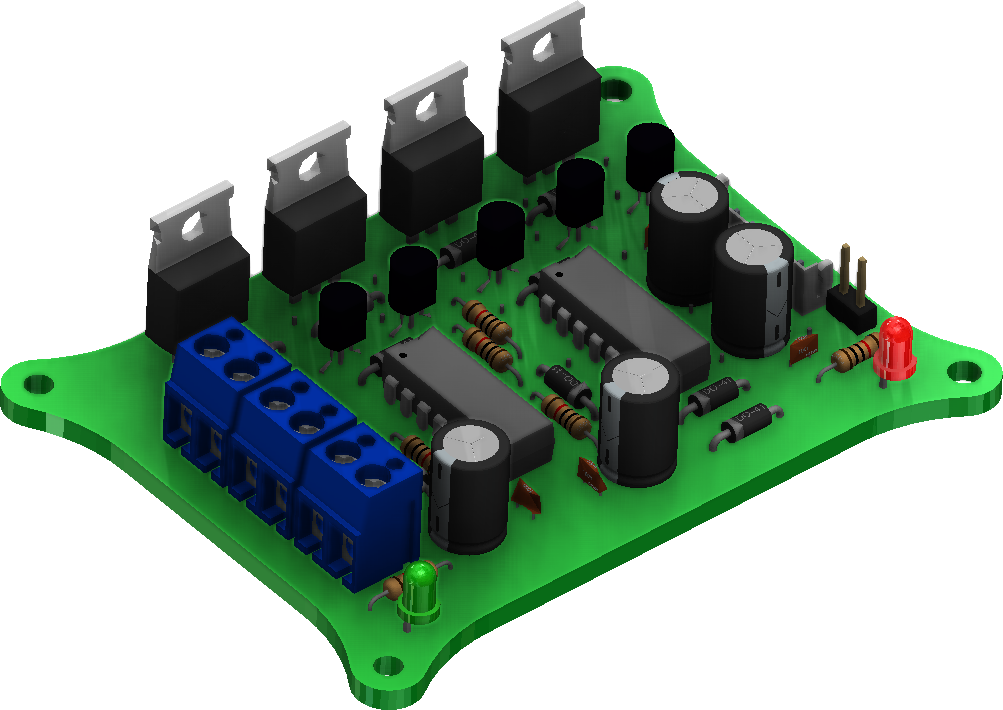
\includegraphics[width=0.4\textwidth]{Images/pcb_3d.png}
        \hspace{1cm}
        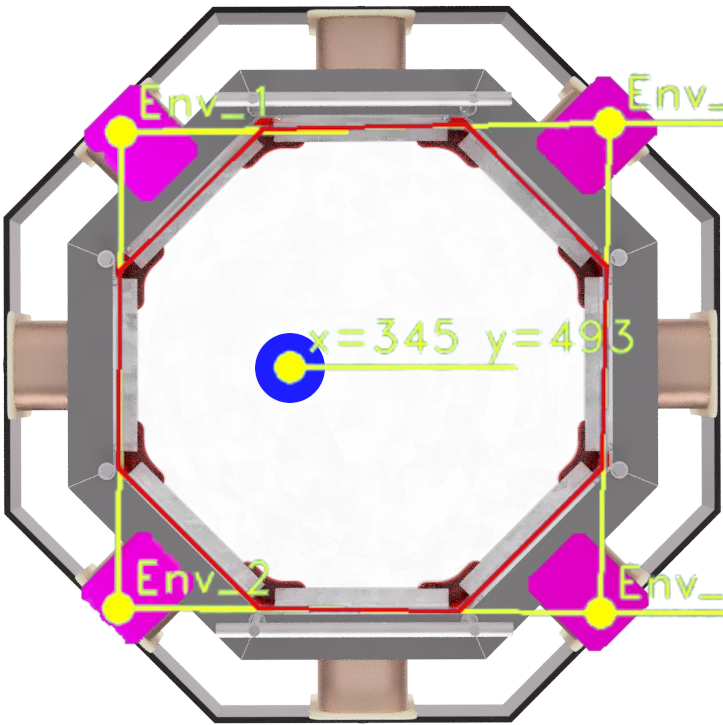
\includegraphics[width=0.3\textwidth]{Images/systeme2-1.png}
    };
\end{tikzpicture}

\begin{minipage}{1.03\textwidth}
% \vspace{1.0cm}
\vspace{1.5cm}
\end{minipage}

\noindent
\vspace{-0.5cm}
\vspace{-1cm}
\fontsize{12}{54}\selectfont
Proposé par : Henrique FAGUNDES-GASPAROTO \\
\fontsize{12}{54}\selectfont
\vspace{1cm}
Thématique : Robotique - Drones \\
\fontsize{12}{15}\selectfont
\underline{Jean Le Bris Domaine professionnel : Cybersécurité} \\
\underline{Ewen Morvan Domaine professionnel : Robotique - Drones}

% Réinitialiser la numérotation à partir de la deuxième page
\clearpage
\pagenumbering{arabic}
% \end{titlepage}
\begin{remerciements}
    Avant de présenter ce rapport, il nous tient particulièrement à coeur de remercier plusieurs personnes sans qui ce projet n'aurait pas avancé aussi loin.
    \\\\
    Tout d'abord, nous souhaiterions remercier Mr. Henrique FAGUNDES GASPAROTO pour avoir proposé ce projet et Mr. Titouan VERDU pour nous avoir aider tout au long du projet.
    \\\\
    Ensuite, nous souhaiterions remercier Mr. Franck LE GALL pour nous avoir donné de précieux conseils sur la partie théorique ainsi que sur le dimensionnement de notre système du point de vue de l'électronique, mais aussi pour nous avoir prêté du matériel de Travaux Pratiques afin de réaliser notre projet.
    \\\\
    Nous tenons aussi à remercier Mr. Jérémy THORAVAL, qui nous a prêté du matériel, qui a été présent tout au long des projets et qui nous a aidé à trouver des solutions quand il y eu des problèmes de commandes.
    \\\\
    Pour finir, nous souhaiterions aussi remercier les employés de la société Estève Recyclage et Tanguy Matériaux pour leur grande générosité, sans qui nous n'aurions pas pu concevoir une structure aussi poussée.
\end{remerciements}

\newpage
\begin{abstract}
La manipulation d'un microrobot magnétique dans l'espace à l'aide d'électro-aimants constitue un domaine de recherche complexe nécessitant une attention particulière pour garantir à la fois le succès de l'opération et l'intégrité du système. Les défis sont nombreux, tant au niveau structurel, électronique que informatique, et la mise en place de mesures de sécurité est essentielle.
\\\\
La conception de la structure requiert une réflexion approfondie : une structure insuffisamment développée pourrait générer des champs magnétiques trop faibles, tandis qu'une structure surdimensionnée pourrait entraîner des coûts excessifs, un facteur crucial lorsque le budget est limité et de nombreux aspects du projet sont onéreux.
\\\\
En ce qui concerne l'électronique, le dimensionnement est crucial : l'absence d'une électronique adéquate rendrait le système inutilisable. Alimenter efficacement huit bobines nécessite la conception de huit systèmes de contrôle de puissance indépendants, avec des composants variés, certains peu coûteux comme les résistances et d'autres plus onéreux comme les drivers ou les PCBs.
\\\\
Quant à l'informatique, une conception minutieuse est indispensable. Bien qu’elle ne coûtent rien à proprement parler, la programmation est essentielle pour résoudre certains problèmes conceptuels. Par exemple, contrôler la vitesse de variation du PWM pour éviter les pics de tension ou surveiller les courants de commande de chaque bobine afin de ne jamais dépasser le courant maximum admissible.
\\\\
Ce projet n'aurait pas pu être réalisé dans les proportions actuelles sans l'aide précieuse de certaines ressources disponibles à l'ISEN, notamment le prêt des bobines. Cependant, étant donné la nature du projet en robotique, l'accès à des matériaux structuraux et à des outils de conception mécanique s'est avéré être un défi de taille. Malheureusement, les démarches classiques proposées par l'ISEN pour l'approvisionnement de ces matériaux se sont avérées insuffisantes. Sans recourir aux matériaux de fabrication et aux outils industriels fournis par des entreprises locales, la réalisation du projet aurait été compromise.

    
\end{abstract}

\newpage
\tableofcontents % Cette commande génère le sommaire automatiquement

\newpage
\section*{Liste des notations}
    
    \begin{itemize}
        \item $B$: Induction magnétique (Teslas, $T$)
        \item $H$: Intensité de champ magnétique (Ampères par mètre, $A/m$)
        \item $\mu_0$: Perméabilité magnétique du vide (Henrys par mètre, $H/m$)
        \item $\mu$ : Moment magnétique (Ampères mètre carre, $A.m^2$)
        \item $\mathcal{M}$ : Aimantation (Ampères par mètre, $A/m$)
        \item $P$ : Poids (Newton, $N$)
        \item $F$ : Force (Newton, $N$)
        \item $m$ : Masse (kilogramme, $Kg$)
        \item $t$ : Temps (secondes, $s$)
        \item $\rho$ : Masse Volumique (kilogramme par mètre cube, $Kg/m^3$)
        \item $S$ : Surface (mètre carre, $m^2$)
        \item $R$ : Rayon (mètre, $m$) ou Résistance (ohm,$\Omega$)
        \item $V$ : Volume (mètre cube, $m^3$)
        \item $\nu$ : Vitesse (mètre par secondes, $m/s$)
        \item $Re$ : Nombre de Reynolds  (sans unité)
        \item $Cx$ : Coefficient de traînée  (sans unité)
        \item $\eta$ : Viscosité cinématique  (mètres carrés par seconde, $m^2/s$)
    \end{itemize}

\listoffigures

%Introduction............................................

\newpage
\section{Introduction}
    La manipulation magnétique sans contact est un sujet d'intérêt en médecine. Elle permet d'intervenir dans le corps humain par le biais de petits agents qui n'ont pas besoin de porter une capacité d'intelligence embarquée (ce qui réduit toute l'électronique embarquée), ce qui peut réduire considérablement la taille de ces petits porteurs. En général, dans ces systèmes, les capacités de perception, d'intelligence et de contrôle de l'action restent extérieures à l'agent.
    \\\\
    Actuellement, l'une des méthodes les plus prometteuses pour cibler efficacement des maladies locales ou le cancer consiste à utiliser des "microrobots" guidés magnétiquement. Plus précisément, le terme "microrobot magnétique" désigne une catégorie de systèmes activés par des champs ou des gradients magnétiques. Cela évite d'avoir recours à des traitements généralisés qui ne détruisent pas uniquement les cellules ciblées.
    \\\\
    Ce projet vise donc à étudier la manipulation magnétique dans un contexte beaucoup plus simple, en essayant de contrôler par des électro-aimants le mouvement d'un petit bateau magnétisés dans un bassin.


\newpage
\section{Gestion du projet}
    \subsection{QQOQCCP}
        \noindent Quoi ? Créer un système de guidage pour un microrobot magnétique.
        \\\\
        Qui ? Les étudiants travaillant sur ce projet (Ewen MORVAN et Jean LE BRIS) ainsi que les responsables du projet (Titouan VERDU et Henrique FAGUNDES GASPAROTO).
        \\\\
        Où ? Au sein de l'ISEN YNCREA Ouest à Brest.
        \\\\
        Quand ? Du 08 janvier 2024 au 19 avril 2024.
        \\\\
        Comment ? En concevant la structure du système, en la fabriquant, en concevant l'électronique et en développant l'informatique.
        \\\\
        Combien ? Un budget de 500€ est alloué au projet.
        \\\\
        Pourquoi ? Pour observer les intérêts que pourrait avoir cette technologie dans divers domaines.

    \subsection{Cahier des Charges}
        \subsubsection*{Contexte et définition du projet}
            \noindent Le but de ce projet est d'asservir en position un microrobot passif magnétique.

        \subsubsection*{Objectif du projet}
            \noindent Le système conçu doit être :
            \\
            \tabto{1cm}Précis.
            \\
            \tabto{1cm}Adaptable.

        \subsubsection*{Description fonctionnelle des besoins}
            \noindent Fonctions principales :
            \\
            \tabto{1cm}Le système doit permettre de déplacer le microrobot.
            \\\\
            Fonctions secondaires :
            \\
            \tabto{1cm}Le système doit pouvoir fonctionner en boucle fermée à l'aide d'une caméra.
            \\
            \tabto{1cm}Le système doit pouvoir faire varier la force exercée sur le drône.
            \\
            \tabto{1cm}Le système doit permettre de déplacer le drône selon un parcours prédéfini.
            \\\\
            Fonctions contraintes :
            \\
            \tabto{1cm}Nous ne pouvons pas interagir avec le drône autrement qu'avec un champ magnétique.

        \subsubsection*{Enveloppe budgétaire}
            \noindent Ce projet possède un budget maximal de 500€, les dépenses suivantes ont été estimées la conception du système.
            \\
            \tabto{1cm}Cuivre - 50€
            \\
            \tabto{1cm}Matériaux pour le châssis - 50€
            \\
            \tabto{1cm}Composants électroniques de prototypage - 0€ si l'ISEN les ont déjà - 20-30€ sinon.
            \\
            \tabto{1cm}Composants électroniques finaux + PCB - 150€
            \\
            \tabto{1cm}Linux embarqué + caméra - 100€

    \subsection{Répartition des tâches}
        La gestion de ce projet a été réalisée principalement avec une méthode agile et une méthode en V dans certaines parties par nécessité, mais elle a tout de même été assez complexe, en effet, les prévisions établies, nos développements et le projet en règle générale a été chamboulé à plusieurs moments. Pour commencer, un diagramme de Gantt avait été établi afin de prévoir l'emploi du temps de notre projet.
    
        \begin{figure}[H]
        \centering
            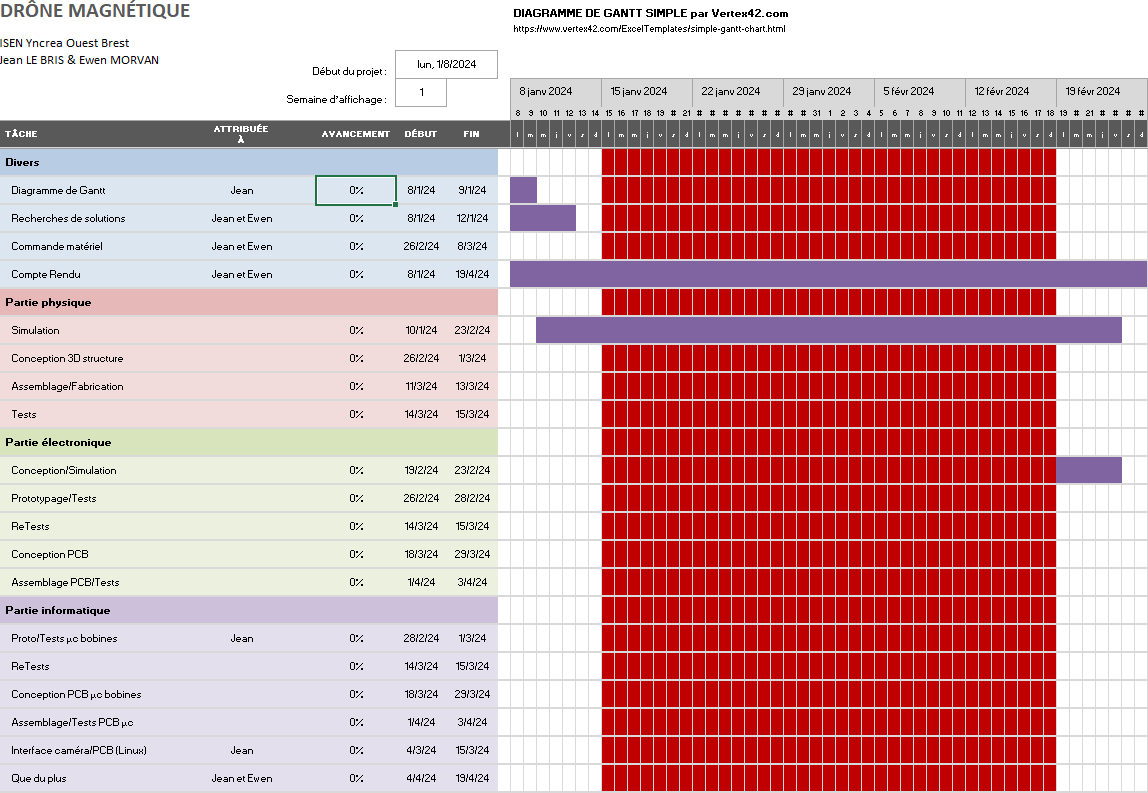
\includegraphics[width = 1\textwidth]{Images/Gantt1.png}
            \caption{Diagramme de Gantt initial partie 1}
            \label{fig:Gantt-1}
        \end{figure}

        \begin{figure}[H]
        \centering
            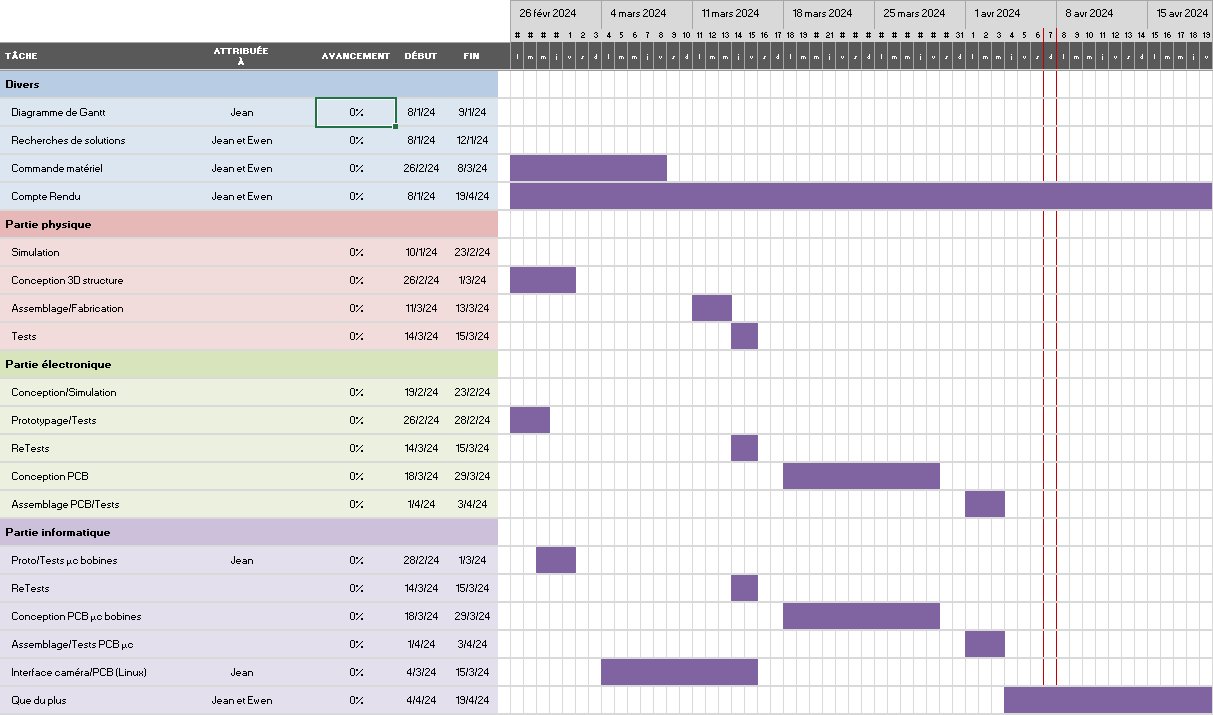
\includegraphics[width = 1\textwidth]{Images/Gantt2.png}
            \caption{Diagramme de Gantt initial partie 2}
            \label{fig:Gantt-2}
        \end{figure}
        
        \noindent Les tâches ont été réparties entre les différents membres du groupe en fonction de leurs compétences respectives, ainsi, Ewen MORVAN se chargea principalement de la conception structurelle et électronique et Jean LE BRIS se chargea principalement de la conception informatique.
        \\\\
        Les délais affichés dans le diagramme de Gantt ont été estimés et parfois surévalués afin d'avoir une marge de manoeuvre.

    \subsection{Déroulement du projet}
        Lors des simulations, le projet s'est bien déroulé, les recherches effectuées afin de comprendre comment faire fonctionner le projet se sont déroulées sans accrocs.
        \\\\
        Néanmoins, après avoir eu des difficultés à contacter le responsable de projet afin de faire part de l'avancement de celui-ci, le 7 mars il nous a fait part d'une meilleure méthode de fonctionnement pour notre système que celui prévu jusqu'alors.
        \\\\
        Ainsi, la conception structurelle et électronique du système ont été recommencés de zéro afin de mettre en place le système que l'on nous a proposé, en effet, ces deux parties étaient les deux parties conçues selon la méthode en V car elles sont intégralement inter-connectées, un changement sur la structure nécessite de redimensionner entièrement l'électronique analogique et un changement sur l'électronique analogique nécessite de modifier la structure pour le considérer.
        
        \begin{figure}[H]
            \centering
                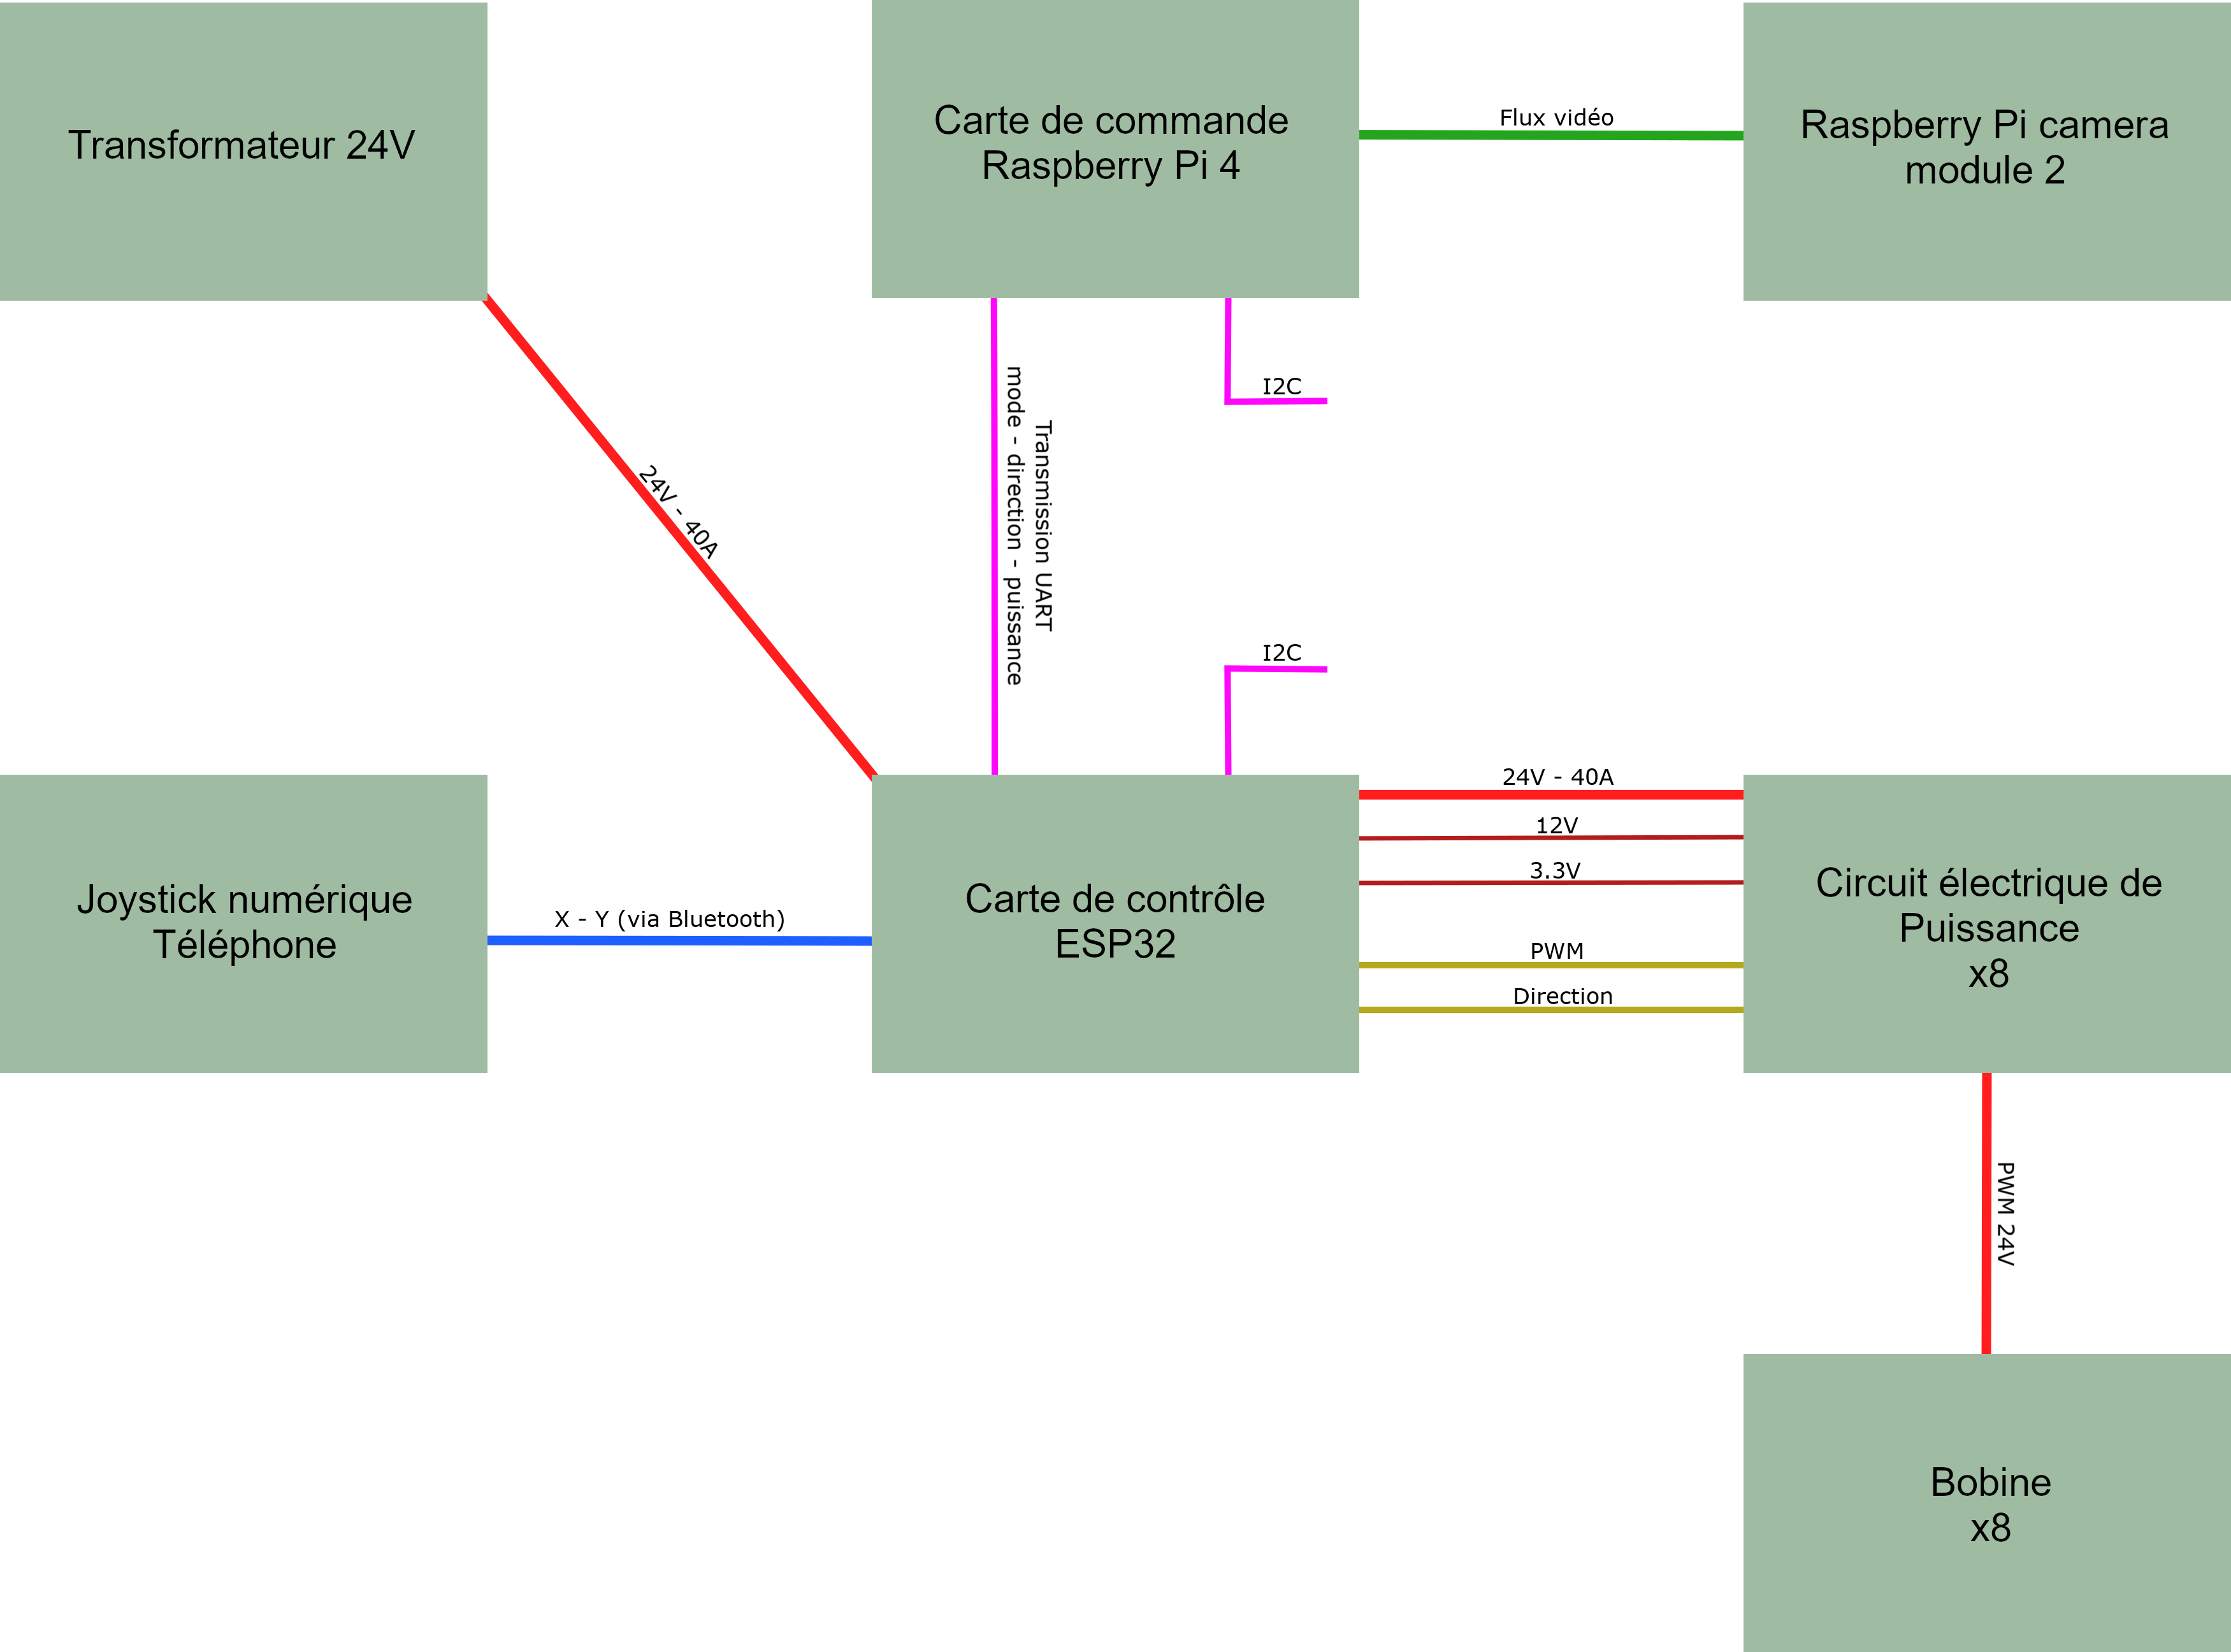
\includegraphics[width = 1\textwidth]{Images/system.png}
                \caption{Méthodologie du système développé}
                \label{fig:methodologie}
        \end{figure}

        \noindent Le nouveau système a pour avantage de permettre de ne pas acheter de grandes quantités de cuivre puisque des bobines de Travaux Pratiques déjà en stock seraient utilisées sur une structure démontable. Heureusement, la recherche théorique restant la même et la conception informatique n'a pas été recommencée de zéro car la programmation, ayant pu être conçue selon la méthode agile est restée relativement similaire avant et après le changement.
        \\\\
        Ainsi, une fois la structure et l'électronique mis a jour, des commandes ont été envoyées pour obtenir les matières premières et les composants nécessaire à la réalisation du projet. Toutefois, les fournisseurs de matières première pour la construction de la structure étant des fournisseurs hors compte, les commandes réalisées auprès d'eux furent refusées, mais après recherches, un fournisseur local pouvant nous fournir l'intégralité des matières première nécessaires pour la construction de la structure a été trouvé, et ce gratuitement. Ainsi nous avons pu construire la structure entière en acier, ainsi que prévoir la construction de l'aquarium en plexiglas en récupérant des cornières en aluminium.
        \\\\
        Alors même que la structure était construite, et que nos modèles électroniques de test fonctionnaient, l'avancement du projet fut retardé par des problèmes de livraison pour les composants électroniques qui furent résolus après deux semaines.

    \subsection{Dépenses réelles du projet}
        \noindent Après le déroulement du projet, il est possible de se rendre compte des dépenses réelles du projet en comparaison aux estimations effectuées.
        \\
        \tabto{1cm}Bobines : 0€, fournies par l'ISEN (valeur : approximativement 2000€).
        \\
        \tabto{1cm}Matériaux pour le châssis : 0€ (Matériaux de récupération ou donnés par un ferrailleur).
        \\
        \tabto{1cm}Composants électroniques : 200€
        \\
        \tabto{1cm}Cartes PCBs : 40€
        \\
        \tabto{1cm}Linux embarqué + caméra : 0€
        \\
        \tabto{1cm}Carte ESP32 : 12€
        \\
        \tabto{1cm}Transformateur : 80€
        \\\\
        Il est ainsi facile de remarquer les différences notables entre les estimations au début du projet, et les dépenses réelles en fin de projet. En effet, les estimations établies se sont avérées loin de la réalité, en particulier pour le cuivre et pour les matériaux du châssis. Réaliser le projet a été rendu possible grâce à la bonté de certains professeurs ayant accepté de nous prêter du matériel coûteux et grâce à des professionnels qui nous ont donné les matériaux dont nous avions besoins.
    
%Propulsion et orientation du microrobot magnétique............................................

\section{Propulsion et orientation du microrobot magnétique}
%\begin{comment}
    Pour déplacer le microrobot, une approche basée sur les champs électromagnétiques a été privilégiée. Cette méthode offre la possibilité d'un contrôle électronique et informatique précis. Dans cette étude, différentes configurations de bobines ont été examinées. Cette section présente une analyse des lois physiques de l'électromagnétisme ainsi que des simulations numériques effectuées à l'aide du logiciel ANSYS Maxwell.

\subsection{Champ Magnétique Créé par une Bobine}
    La loi de Biot-Savart \cite{ref2} est utilisée pour calculer le champ magnétique $\mathbf{B}$ en un point $\mathbf{r}$ dans l'espace généré par un courant électrique le long d'un fil. Cette loi s'exprime par l'équation :
    \begin{equation}
    \mathbf{B}(\mathbf{r}) = \frac{\mu_0}{4\pi} \oint \frac{I \, d\mathbf{l} \times \mathbf{r'}}{| \mathbf{r'}|^3}\label{eq:Boit_Savart}
    \end{equation}
    où $\mu_0$ est la perméabilité magnétique du vide, $I$ est le courant dans le fil, $d\boldsymbol{\ell}$ est un élément de longueur le long du fil, et $\mathbf{r'}$ est le vecteur de déplacement du fil au point où le champ est calculé.\\\\
    Dans le cas d'une bobine de $n$ spires de rayon $R$ parcourue par un courant $I$, à une distance $z$ de la ligne centrale de la bobine, le champ magnétique $B$ s'écrit :
    \begin{equation}
       \mathbf{B}(z) = \frac{\mu_0nIR^{2}}{2(R^{2}+z^{2})^{\frac{3}{2}}}\label{eq:Equation2}
    \end{equation}

    \begin{figure}[H] % Utilisation de la position H pour forcer la positionnement de la figure ici
        \centering
        
        \begin{minipage}{0.55\textwidth}
        \hspace{0.5cm}
        \begin{tikzpicture}
            \begin{axis}[
                axis lines = left,
                xlabel = \(z\) (m),
                ylabel = {\(\mathbf{B}(z)\) (T)},
                legend pos = south east,
            ]
            % Below the red parabola is defined
            \addplot [
                domain=-0.5:0.5, 
                samples=100, 
                color=green,
            ]
            {(0.0000012*10*1*0.1^2)/(2*(0.1^2+x^2)^(3/2))};
            \addlegendentry{\(R=0.1 \, \text{m}, I=1 \, \text{A} , n=10\)}
            \end{axis}
        \end{tikzpicture}
            \end{minipage}%
        \begin{minipage}{0.5\textwidth}
            \centering
            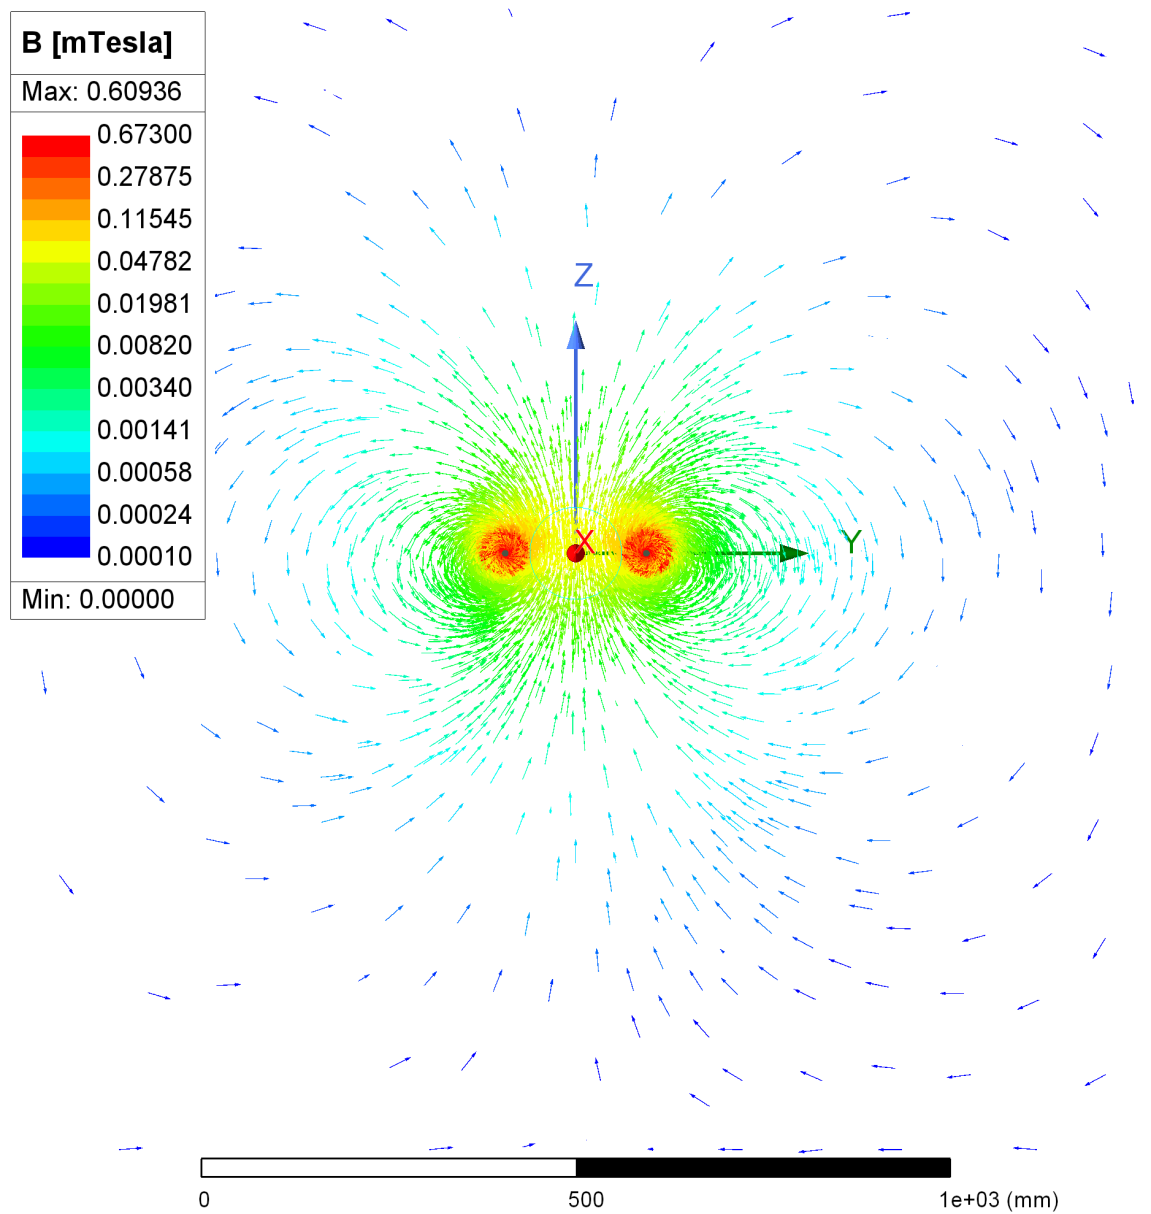
\includegraphics[width=8.5cm]{Images/Bobine simple4.png}
            \end{minipage}
            \caption{Intensité en fonction de $\mathbf{z}$ et visualisation 2D du champ magnétique $\mathbf{B}$ créé par une bobine.}
            \label{fig:champB_1Bobine}
        \end{figure}
\noindent
L'intensité du champ magnétique $\mathbf{B}$ décroît notablement avec l'augmentation de la distance $\mathbf{z}$. De plus, comme illustré dans la simulation \ref{fig:champB_1Bobine}, les lignes de champ sont uniformes dans la direction de l'axe de la bobine et dévient pour boucler du pôle Nord au pôle Sud de la bobine. L'orientation des champs de manière uniforme dans la direction souhaitée faciliterait le déplacement du microrobot.\\
        \noindent
       Une méthode simple pour créer un champ magnétique uniforme consiste à utiliser un solénoïde. En effet, les champs $\mathbf{B}$ s'additionnent, ce qui crée un champ uniforme au centre du solénoïde. 
        \begin{figure}[h] % Positionnement de la figure
            \centering
            % Inclure une image
            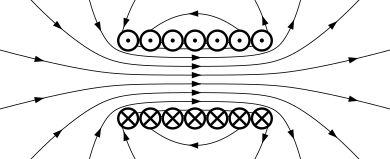
\includegraphics[width=0.3\textwidth]{Images/Solenoid.png}
            \caption{Champ magnétique créé par un solénoïde \cite{ref5}.}
            \label{fig:image}
        \end{figure}\\
\noindent
Cependant, à grande échelle, cette approche est très encombrante et ne laisse pas suffisamment d'espace pour déplacer le microrobot. De plus, étant donné que le microrobot doit être déplacé suivant deux axes, il semble complexe de positionner deux solénoïdes de manière à obtenir un champ dans chaque direction.
        
\subsection{Bobines d'Helmholtz et de Maxwell}
    Afin d'obtenir un champ magnétique avec une direction uniforme et un espace de travail dégagé, les bobines d'Helmholtz représentent une solution prometteuse. En effet, grâce au principe de superposition (\( \mathbf{B_{\text{Helmholtz}}} = \mathbf{B_{1}} + \mathbf{B_{2}} \)), il est possible d'additionner les champs magnétiques de deux bobines. Si deux bobines de rayon \( R \) sont placées face à face aux positions \( -\frac{R}{2} \) et \( \frac{R}{2} \), alors d'après l'équation \eqref{eq:Equation2}, leur champ résultant sera :

    \begin{equation}
        \mathbf{B_{Helmholtz}(z)} = \frac{\mu_0nIR^{2}}{2(R^{2}+(z-\frac{R}{2})^{2})^{\frac{3}{2}}} + \frac{\mu_0nIR^{2}}{2(R^{2}+(z+\frac{R}{2})^{2})^{\frac{3}{2}}}\label{eq:Equation3}
    \end{equation}
    
    
    \begin{figure}[H] % Utilisation de la position H pour forcer la positionnement de la figure ici
        \centering
        
        \begin{minipage}{0.55\textwidth}
            \hspace{0.5cm}
            \begin{tikzpicture}
                \begin{axis}[
                    axis lines = left,
                    xlabel = \(z\) (m),
                    ylabel = {\(\mathbf{B}(z)\) (T)},
                    legend pos = south east,
                ]
                % Below the red parabola is defined
                \addplot [
                    domain=-0.3:0.3, 
                    samples=100, 
                    color=green,
                ]
                {(0.0000012*10*1*0.1^2)/(2*(0.1^2+(x-0.05)^2)^(3/2))};
                \addlegendentry{\(B_{1}\)}
                \addplot [
                    domain=-0.3:0.3, 
                    samples=100, 
                    color=orange,
                ]
                {(0.0000012*10*1*0.1^2)/(2*(0.1^2+(x+0.05)^2)^(3/2))};
                \addlegendentry{\(B_{2}\)}
                \addplot [
                    domain=-0.3:0.3,  
                    samples=100, 
                    color=blue,
                ]
                {(0.0000012*10*1*0.1^2)/(2*(0.1^2+(x-0.05)^2)^(3/2))+(0.0000012*10*1*0.1^2)/(2*(0.1^2+(x+0.05)^2)^(3/2))};
                \addlegendentry{\(B_{\text{Helmholtz}}\)}
                \end{axis}
            \end{tikzpicture}
        \end{minipage}%
        \begin{minipage}{0.5\textwidth}
            \centering
            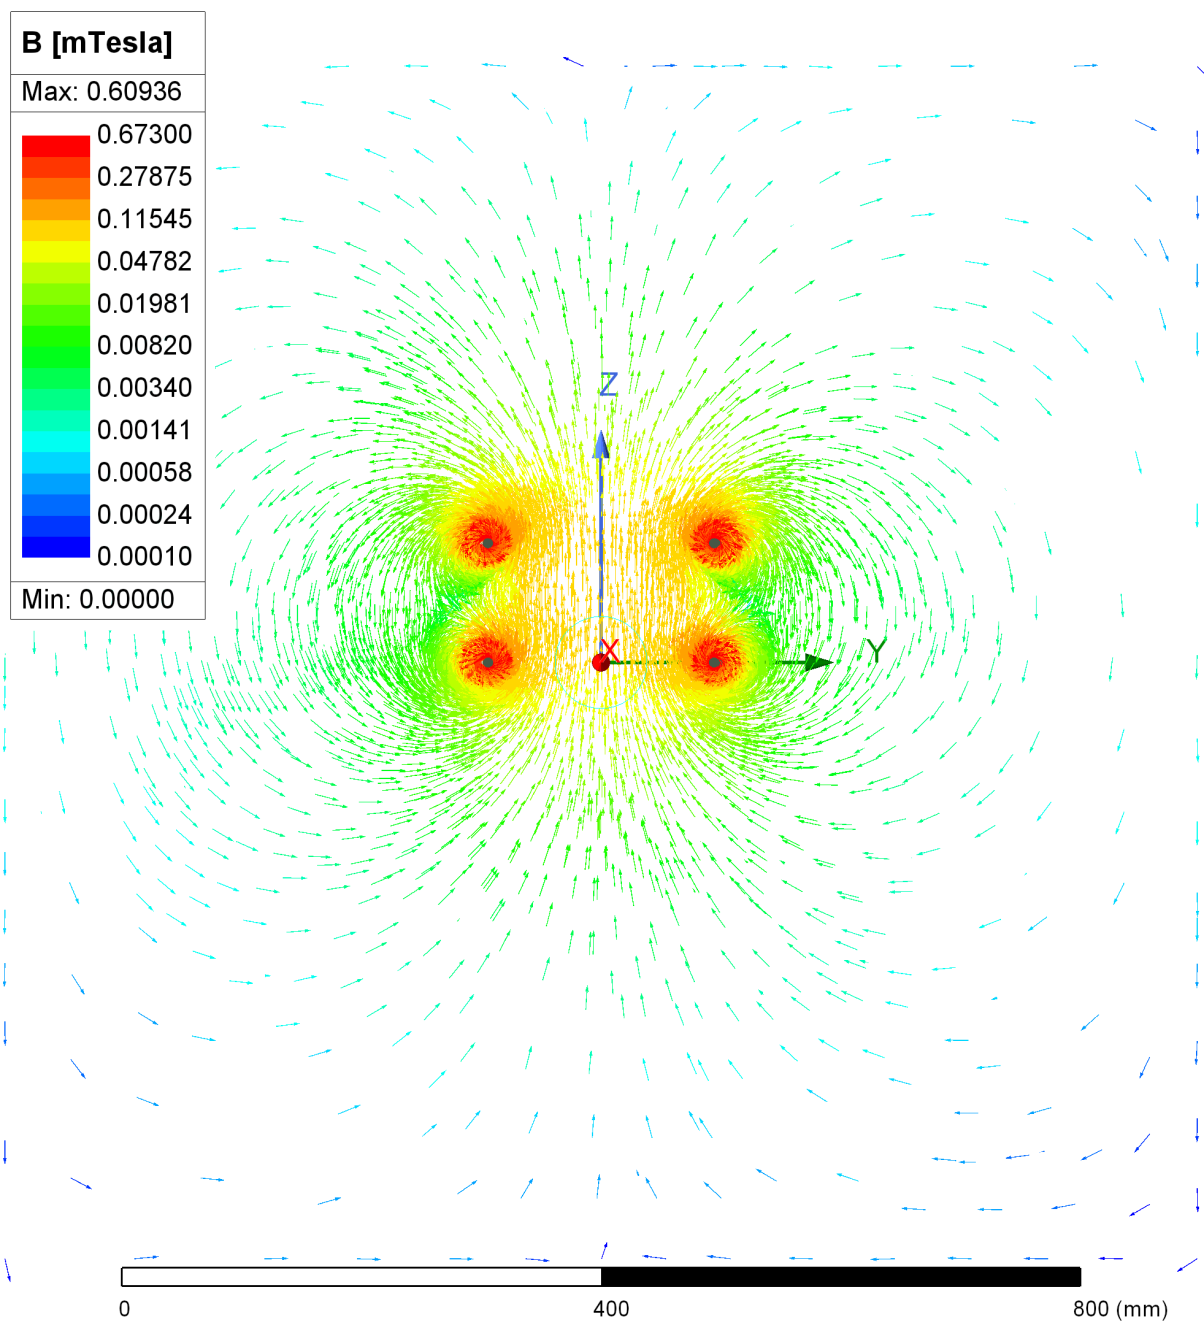
\includegraphics[width=8.5cm]{Images/Helmotz1A2.png}
        \end{minipage}
        \caption{Intensité en fonction de $\mathbf{z}$ et visualisation 2D du champ magnétique $\mathbf{B}$ créé par deux bobine.}
        \label{fig:champB_2Bobine}
    \end{figure}
\noindent
La configuration de Helmotz présente plusieurs avantages : elle est relativement simple à réaliser et offre un espace de travail assez vaste. Il est également possible de croiser deux paires de bobines de Helmotz pour obtenir un champ uniforme orientable en deux dimensions. Un système similaire à celui représenté dans l'image \ref{fig:sytèmeV1} a été envisagé. Dans ce schéma, le bac central représente la zone remplie d'eau où le microrobot évoluera. Des bobines de Helmotz carrées ont été utilisées afin de s'encaster sans réduire significativement le volume utile de travail. Comme la forme carrée est symétrique, le champ magnétique créé se comporte de la même manière que précédemment. Seule l'intensité varie légèrement, mais cela reste prévisible grâce aux simulations numériques.

    \begin{figure}[H] % Utilisation de la position H pour forcer la positionnement de la figure ici
        \centering
        \begin{minipage}{0.5\textwidth}
            \centering
            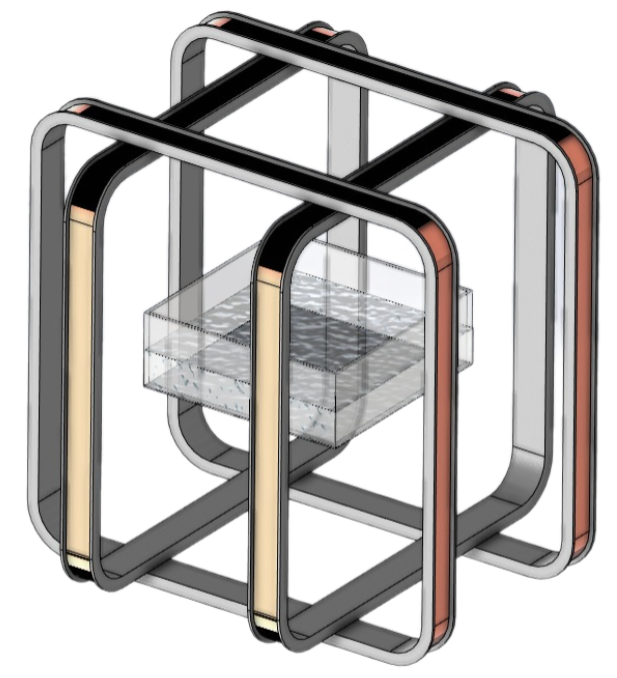
\includegraphics[width=5cm]{Images/ProtoV1.png}
        \end{minipage}%
        \begin{minipage}{0.5\textwidth}
            \centering
            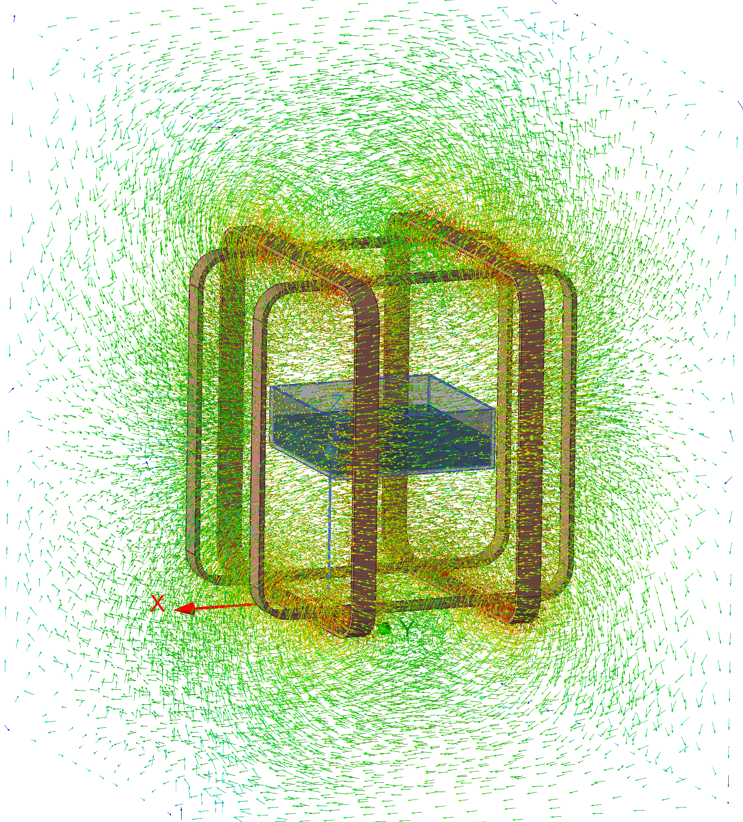
\includegraphics[width=6.5cm]{Images/PhotoTitreProvisoir.png}
        \end{minipage}
        \caption{Visualisation 3D du premier système envisagé avec une double paire de bobines de Helmotz, accompagnée d'une simulation numérique illustrant son champ $\mathbf{B}$.}
        \label{fig:sytèmeV1}
    \end{figure}
\noindent
Ce système permet ainsi de générer un champ uniforme en direction et en intensité au niveau de la zone de travail (le bac d'eau). De plus, en ajustant l'intensité dans les différentes paires de bobines, il est possible de créer un champ magnétique tournant à 360°. Cela offre la possibilité d'orienter le microrobot de la même manière qu'une boussole. En effet, l'aimant permanent contenu dans le microrobot possède un moment magnétique. Cette formule \cite{ref4} permet de calculer le couple appliquer sur l'aimant:
    \begin{equation}
      \vec{\tau} = \vec{\mu} \wedge \vec{B}\label{eq:coupleMomentMag}
    \end{equation}
     où $\vec{\mu}$ représente le moment magnétique du dipôle et $\vec{B}$ le champ magnétique externe. Ainsi, avec les propriétés du produit vectoriel, cela implique que l'aimant subit un couple tant que son moment magnétique n'est pas aligné avec le champ $\vec{B}$.

    \begin{figure}[H]
        \centering
        % \includegraphics{}
         \animategraphics[width=\textwidth, loop, autoplay]{5}%frame rate
        {Images/GifChampTournant/Proto1Img}%path to figures
        {0}%start index
        {17}%end index
        \caption{Animation du champ magnétique rotatif.}


        \label{fig:my_label}
    \end{figure}
    {\small\itshape\color{gray} Cette animation fonctionnera uniquement dans Acrobat Reader. Si vous ne l'avez pas, vous pouvez la télécharger \href{https://drive.google.com/file/d/1W6Fok3klrCoOXPwF3TfWwfjug8hkEbIQ/view?usp=drive_link}{ICI}.}
    \\\\
    Malheureusement, ce système ne pourra pas fonctionner tel quel car il permet uniquement d'orienter l'aimant mais pas de le propulser. En effet, la formule de la force appliquée à un dipôle magnétique \cite{ref4} est la suivante :
    \begin{equation}
      \vec{F} = \vec{\nabla} (\vec{\mu} \cdot \vec{B}) \label{eq:ForceMag}
    \end{equation}
    \noindent
    Puisque $\vec{\mu}$ est constant car l'aimant est permanent, cela implique que le gradient s'applique forcément à $\vec{B}$, sinon la force est nulle. Or, dans le système précédent (voir figure \ref{fig:sytèmeV1}), le champ est uniforme en direction mais aussi en intensité, ce qui signifie que le gradient de $\vec{B}$ est nul, donc la force aussi. Pour s'en convaincre, détaillons le calcul sur l'axe $\mathbf{x}$ par exemple :
    
    % 1. Sur l'axe x :
    \begin{align*}
        \nabla(\boldsymbol{\mu}\cdot\mathbf{B})_x &= \frac{\partial}{\partial x}(\boldsymbol{\mu}\cdot\mathbf{B}) \\
        &= \frac{\partial}{\partial x}(\vec{\mu}_x \cdot \vec{B}_x + \vec{\mu}_y \cdot \vec{B}_y + \vec{\mu}_z \cdot \vec{B}_z) \\
        &= \frac{\partial\vec{\mu}_x}{\partial x} \cdot \vec{B}_x + \vec{\mu}_x \cdot \frac{\partial\vec{B}_x}{\partial x} + \frac{\partial\vec{\mu}_y}{\partial x} \cdot \vec{B}_y + \vec{\mu}_y \cdot \frac{\partial\vec{B}_y}{\partial x} + \frac{\partial\vec{\mu}_z}{\partial x} \cdot \vec{B}_z + \vec{\mu}_z \cdot \frac{\partial\vec{B}_z}{\partial x}
    \end{align*}
Considérons que l'aimant est aligné dans la direction du champ (en $\mathbf{x}$). Cela implique que $\vec{\mu}_y = \vec{\mu}_z = 0$ et $\vec{\mu}_x = \text{cst}$ car l'aimant est permanent.\\
Donc: 
    \begin{equation}
        \vec{F} = \mu_x \frac{\partial\vec{B}_x}{\partial x}
    \end{equation}
La force $\vec{F}$ est donc proportionel a la dériver du champ magnétique. En ajoutant la dériver sur le graphqiue \ref{fig:champB_2Bobine} il vient:\\\\
 
    \begin{figure}[H]
        \centering
        \begin{tikzpicture}
        
            \begin{axis}[
                axis lines = left,
                xlabel = \(z\) (m),
                ylabel = {\(\mathbf{B}(z)\) (T)},
                legend pos = south east,
            ]
            \addplot [
                domain=-0.3:0.3, 
                samples=100, 
                color=blue,
            ]
            {(0.0000012*10*1*0.1^2)/(2*(0.1^2+(x-0.05)^2)^(3/2))+(0.0000012*10*1*0.1^2)/(2*(0.1^2+(x+0.05)^2)^(3/2))};
            \addlegendentry{\(B_{\text{Helmholtz}}\)}
            \end{axis}
            
            \begin{axis}[
                axis lines = right,
                xlabel = \(z\) (m),
                ylabel = {\(\mathbf{Gard}(B(z))\)},
                legend pos = north east,
                hide x axis,
            ]
            % Plot de la dérivée
            \addplot [
                domain=-0.3:0.3,  
                samples=100, 
                color=red,
            ]
            {-(0.00000009*(2*x-0.1))/(x^2-0.1*x+0.0125)^(5/2)-(0.00000009*(2*x+0.1))/(x^2+0.1*x+0.0125)^(5/2)};
            \addlegendentry{\(\frac{\partial B_{\text{Helmholtz}}}{\partial z}\)}
            \end{axis}
            
        \end{tikzpicture}
        \caption{Champ magnétique résultant et sa dérivée issu de Bobines de Helmotz espacées d'une distance de \(R\)}
    \end{figure}
\noindent
La courbe rouge (le gradient de $\mathbf{B(z)}$ et donc la force qui en découle) montre un comportement nul au centre des bobines, non constant et de sens inverse si le microrobot se rapproche de l'une ou de l'autre bobine.\\
\noindent
La configuration des bobines de Helmotz est donc adaptée à l'orientation du microrobot mais ne l'est donc pas à la propulsion.
        \\\\
        Une autre alternative consiste à utiliser un type de bobine pratiquement similaire, appelé bobines de Maxwell \cite{ref6}. La principale différence est qu'elles sont séparées d'une distance de \(\sqrt{3}R\) et que les courants circulant dans ces bobines sont de sens contraire.

        \begin{figure}[H]
            \centering
            \begin{subfigure}[b]{0.45\textwidth}
                \centering
                \hspace{-2.0cm}
                \begin{tikzpicture}
                    \begin{axis}[
                        axis lines = left,
                        xlabel = \(z\) (m),
                        ylabel = {\(\mathbf{B}(z)\) (T)},
                        legend pos = south east,
                    ]
                   \addplot [
                        domain=-0.3:0.3, 
                        samples=100, 
                        color=green,
                    ]
                    {(0.0000012*10*1*0.1^2)/(2*(0.1^2+(x-0.0866)^2)^(3/2))};
                    \addlegendentry{\(B_{1}\)}
                    \addplot [
                        domain=-0.3:0.3, 
                        samples=100, 
                        color=orange,
                    ]
                    {(0.0000012*10*1*0.1^2)/(2*(0.1^2+(x+0.0866)^2)^(3/2))};
                    \addlegendentry{\(B_{2}\)}
                    \addplot [
                        domain=-0.3:0.3, 
                        samples=100, 
                        color=blue,
                    ]
                    {(0.0000012*10*1*0.1^2)/(2*(0.1^2+(x-0.0866)^2)^(3/2))+(0.0000012*10*1*0.1^2)/(2*(0.1^2+(x+0.0866)^2)^(3/2))};
                    \addlegendentry{\(B_{\text{Maxwell}}\)}
                    \end{axis}
                \end{tikzpicture}
                \centering
                \caption{$I_{B_{1}} = I_{B_{2}}$}
          
            \end{subfigure}
            \hspace{0.05\textwidth} % Espacement horizontal entre les sous-figures
            \begin{subfigure}[b]{0.45\textwidth}
                \centering 
                \begin{tikzpicture}
                    \begin{axis}[
                        axis lines = left,
                        xlabel = \(z\) (m),
                        ylabel = {\(\mathbf{B}(z)\) (T)},
                        legend pos = south east,
                    ]
                    \addplot [
                        domain=-0.3:0.3, 
                        samples=100, 
                        color=green,
                    ]
                    {(0.0000012*10*1*0.1^2)/(2*(0.1^2+(x-0.0866)^2)^(3/2))};
                    \addlegendentry{\(B_{1}\)}
                    \addplot [
                        domain=-0.3:0.3, 
                        samples=100, 
                        color=orange,
                    ]
                    {-(0.0000012*10*1*0.1^2)/(2*(0.1^2+(x+0.0866)^2)^(3/2))};
                    \addlegendentry{\(B_{2}\)}
                    \addplot [
                        domain=-0.3:0.3, 
                        samples=100, 
                        color=blue,
                    ]
                    {(0.0000012*10*1*0.1^2)/(2*(0.1^2+(x-0.0866)^2)^(3/2))-(0.0000012*10*1*0.1^2)/(2*(0.1^2+(x+0.0866)^2)^(3/2))};
                    \addlegendentry{\(B_{\text{Maxwell}}\)}
                    \end{axis}
                \end{tikzpicture}
                \centering
                \caption{$I_{B_{1}} = - I_{B_{2}}$}
             
            \end{subfigure}
            \caption{Champ magnétique résultant issu de bobines de Maxwell espacées d'une distance de $\sqrt{3}R$}
            \label{fig:graphs_maxwell}
        \end{figure}

        \begin{figure}[H]
            \centering
            \begin{subfigure}[b]{0.45\textwidth}
                \centering
                \hspace{-2.0cm}
                \begin{tikzpicture}
                    \begin{axis}[
                        axis lines = left,
                        xlabel = \(z\) (m),
                        ylabel = {\(\mathbf{B}(z)\) (T)},
                        legend pos = south east,
                    ]
                    \addplot [
                        domain=-0.3:0.3, 
                        samples=100, 
                        color=blue,
                    ]
                    {(0.0000012*10*1*0.1^2)/(2*(0.1^2+(x-0.0866)^2)^(3/2))+(0.0000012*10*1*0.1^2)/(2*(0.1^2+(x+0.0866)^2)^(3/2))};
                    \addlegendentry{\(B_{\text{Maxwell}}\)}
                    \end{axis}
                    \begin{axis}[
                        axis lines = right,
                        xlabel = \(z\) (m),
                        ylabel = {\(\mathbf{Gard}(B(z))\)},
                        legend pos = north east,
                        hide x axis,
                    ]
                    \addplot [
                        domain=-0.3:0.3, 
                        samples=100, 
                        color=red,
                    ]
                    {-(0.00000009*(2*x-0.1732))/(x^2-0.1732*x+0.01749)^(5/2)-(0.00000009*(2*x+0.1732))/(x^2+0.1732*x+0.017499)^(5/2)};
                    \addlegendentry{\(\frac{\partial B_{\text{Maxwell}}}{\partial z}\)}
                    \end{axis}
                \end{tikzpicture}
                \centering
                \caption{$I_{B_{1}} = I_{B_{2}}$}
         
            \end{subfigure}
            \hspace{0.05\textwidth} % Espacement horizontal entre les sous-figures
            \begin{subfigure}[b]{0.45\textwidth}
                \centering 
                \begin{tikzpicture}
                    \begin{axis}[
                        axis lines = left,
                        xlabel = \(z\) (m),
                        ylabel = {\(\mathbf{B}(z)\) (T)},
                        legend pos = south east,
                    ]
                    \addplot [
                        domain=-0.3:0.3, 
                        samples=100, 
                        color=blue,
                    ]
                    {(0.0000012*10*1*0.1^2)/(2*(0.1^2+(x-0.0866)^2)^(3/2))-(0.0000012*10*1*0.1^2)/(2*(0.1^2+(x+0.0866)^2)^(3/2))};
                    \addlegendentry{\(B_{\text{Maxwell}}\)}
                    \end{axis}
                    \begin{axis}[
                        axis lines = right,
                        xlabel = \(z\) (m),
                        ylabel = {\(\mathbf{Gard}(B(z))\)},
                        legend pos = north east,
                        hide x axis,
                    ]
                    \addplot [
                        domain=-0.5:0.5, 
                        samples=100, 
                        color=red,
                    ]
                    {-(0.00000009*(2*x-0.1732))/(x^2-0.1732*x+0.01749)^(5/2)+(0.00000009*(2*x+0.1732))/(x^2+0.1732*x+0.017499)^(5/2)};
                    \addlegendentry{\(\frac{\partial B_{\text{Maxwell}}}{\partial z}\)}
                    \end{axis}
                \end{tikzpicture}
                \centering
                \caption{$I_{B_{1}} = - I_{B_{2}}$}
                
            \end{subfigure}
            \caption{Champ magnétique résultant et leur gradient issus de bobines de Maxwell espacées d'une distance de $\sqrt{3}R$}
            \label{fig:graphs_grad_maxwell}
        \end{figure}

        
\begin{figure}[H] % Utilisation de la position H pour forcer la positionnement de la figure ici
      
            \centering
            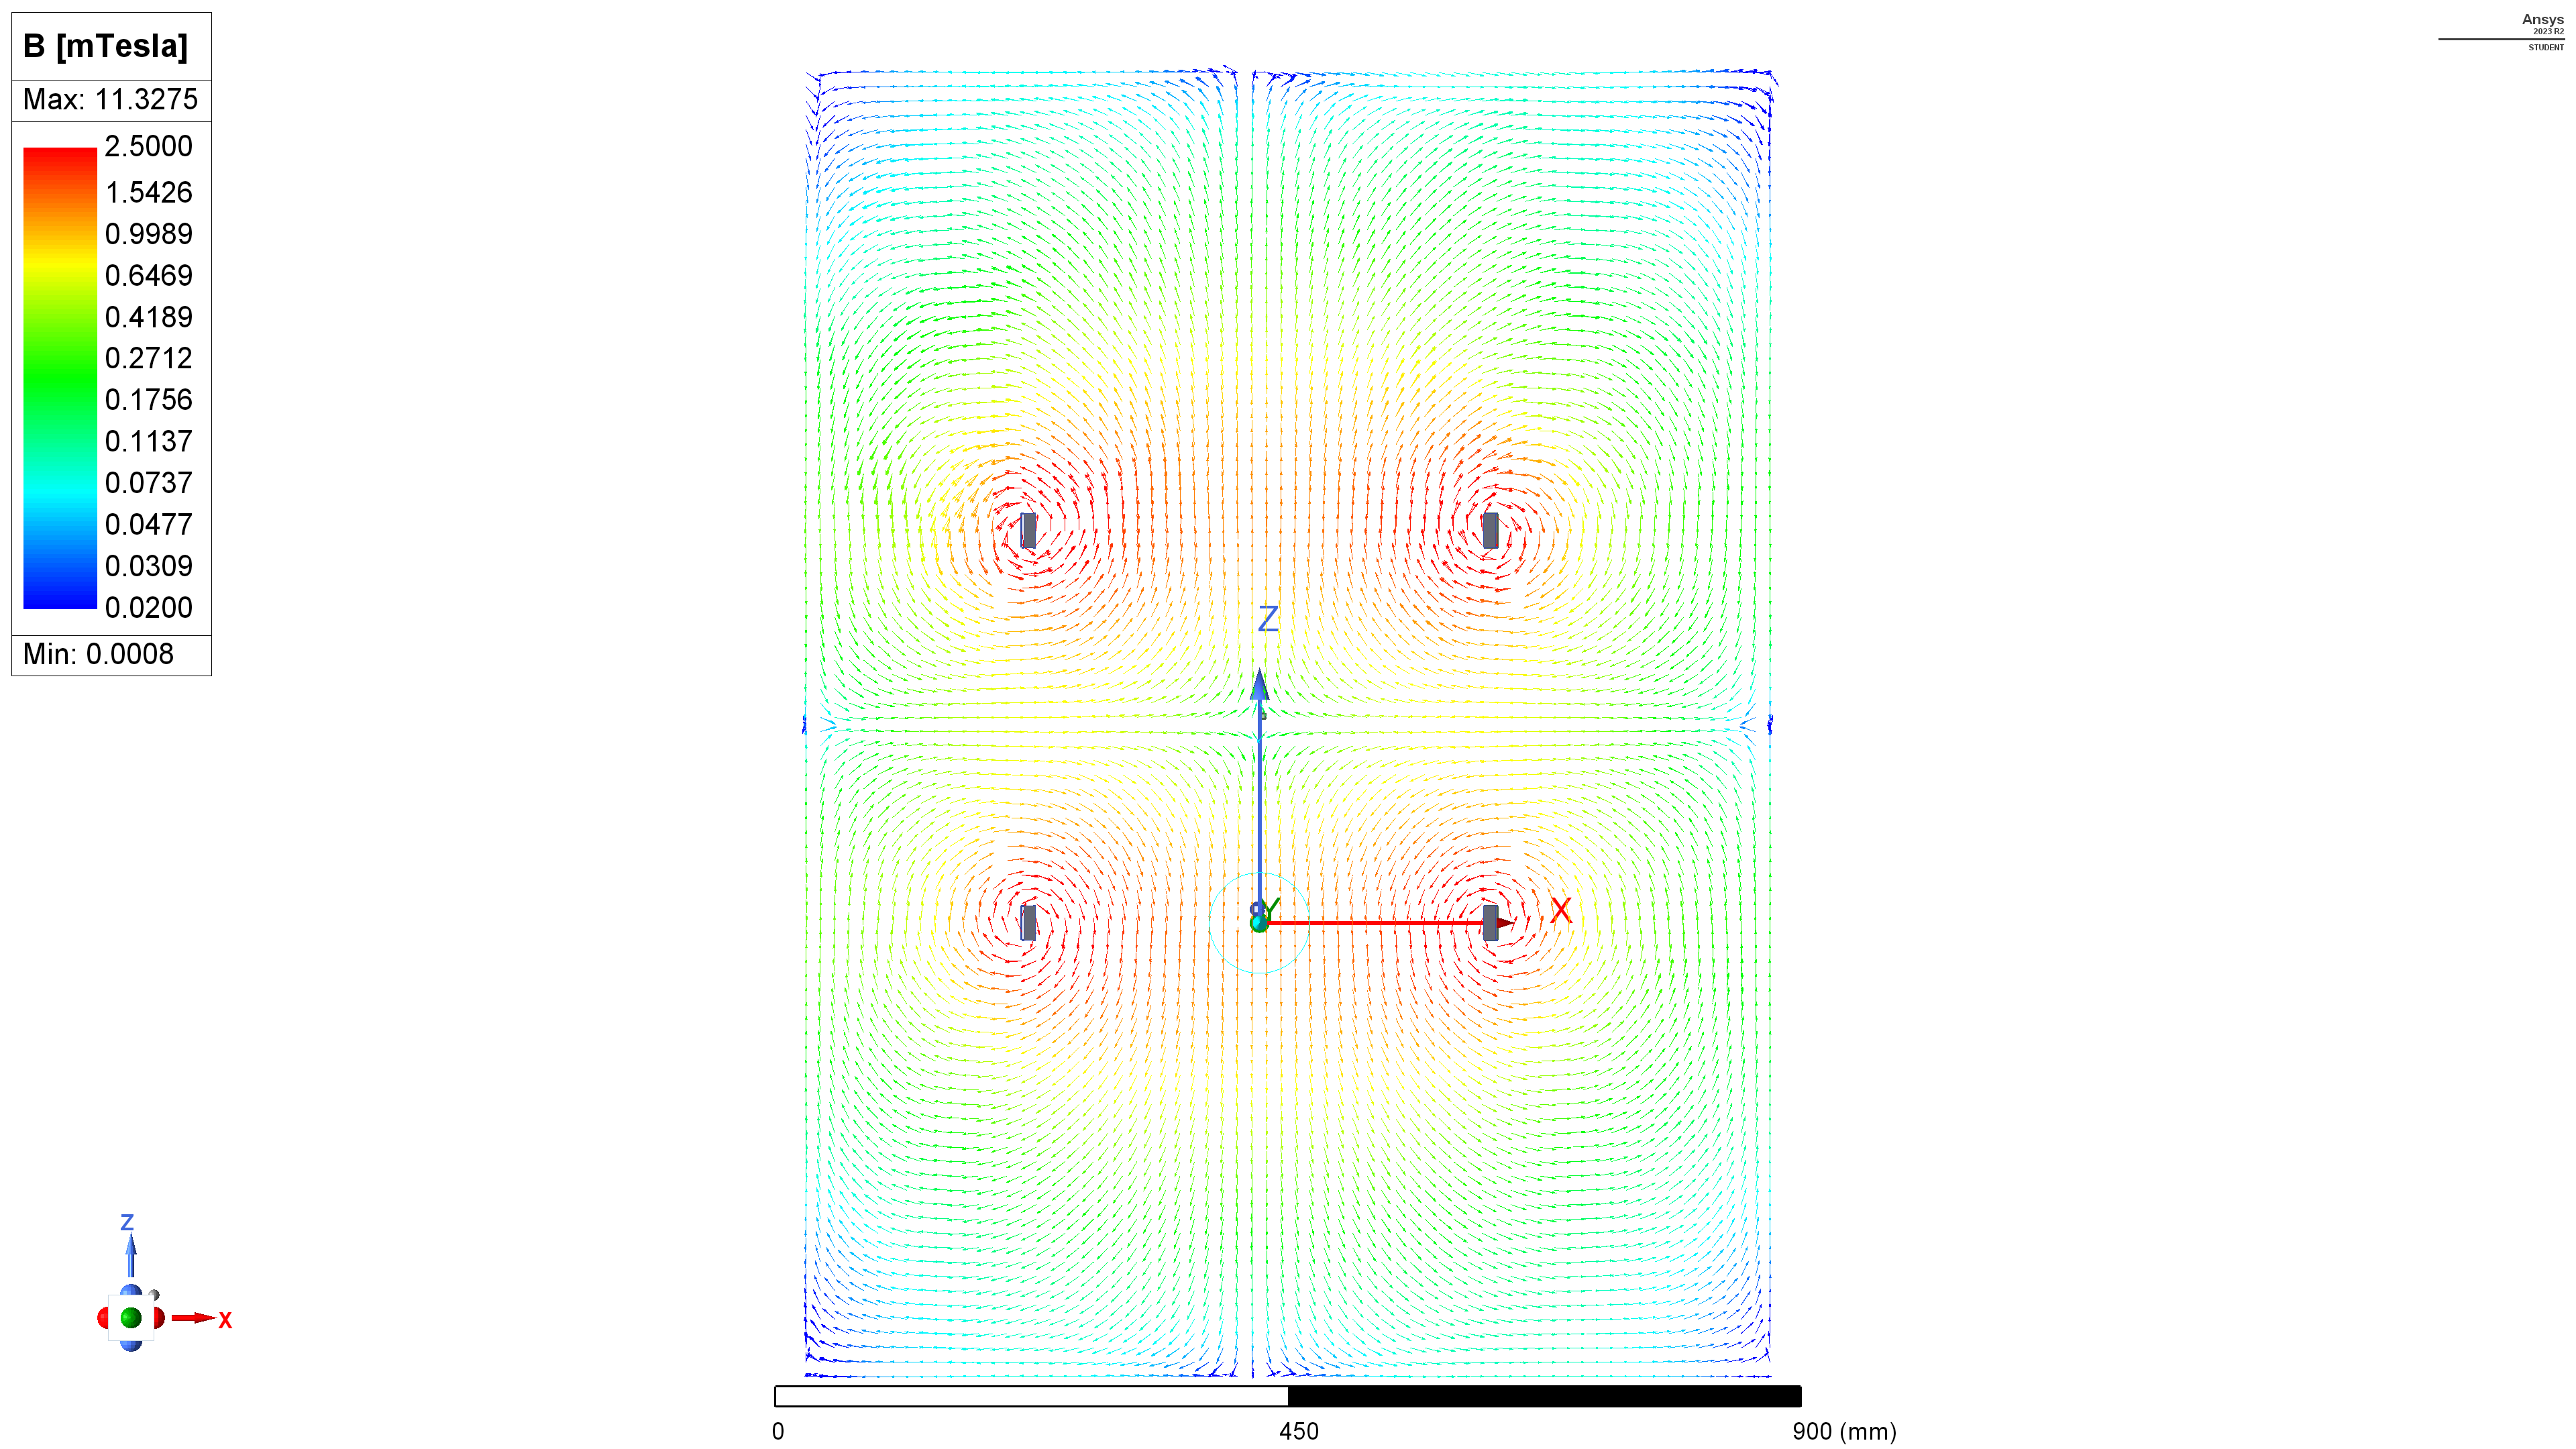
\includegraphics[width=15cm]{Images/bobineMaxewll1.png}
       
        \caption{Simulation numérique du champ magnétique d'une paire de bobines de Maxwell, parcourue par des courrant de sens opposer}
        \label{fig:GradMaxwell}
    \end{figure}
\noindent
Les données présentées dans les figures \ref{fig:graphs_maxwell} et \ref{fig:graphs_grad_maxwell} démontrent une uniformité du gradient sur l'axe Z entre les bobines. Cette caractéristique, conforme à l'équation de la force magnétique  \ref{eq:ForceMag}, présente des avantages pour la propulsion.\\
Cependant, des problèmes subsistent. L'aimant permanent, tend à s'aligner avec le champ magnétique environnant, comme évoqué précédemment. Malgré la constance du gradient et sa direction uniforme, le champ magnétique oscille entre des polarités négatives et positives. Par conséquent, selon la proximité de l'aimant par rapport à chacune des bobines, celui-ci s'alignera initialement avec le champ généré par la bobine la plus proche avant de s'en rapprocher. Une solution envisagée consiste à maintenir une configuration similaire, mais en évitant d'allumer simultanément les bobines d'une même paire. En d'autres termes, lorsqu'une bobine est activée, l'aimant se dirigera vers celle-ci. Cette approche maintient la direction du champ magnétique $\mathbf{B}$ inchangée le long de l'axe de déplacement, mais induit un gradient qui n'est plus constant, entraînant ainsi une variation de la force exercée.

\subsection{Dimensionnement et conception du système d'actionnement électromagnétique}
À ce stade, afin de prendre en compte les contraintes exposées dans la section précédente, la première idée de conception (voir figure \ref{fig:sytèmeV1}) a été légèrement modifiée. L'objectif était d'avoir quatre bobines indépendantes suffisamment écartées de l'aquarium pour éviter le problème de déviation de l'aimant sur les côtés des bobines. L'idée est d'allumer une bobine à la fois pour un mouvement le long d'un seul axe du plan, ou une bobine de chaque paire pour un mouvement le long des deux axes du plan.\\\\
En écartant les bobines du bassin, le problème "d'encastrement" est résolu, ce qui permet l'utilisation de bobines rondes et facilite la fabrication .

    \begin{figure}[H]
        \centering
            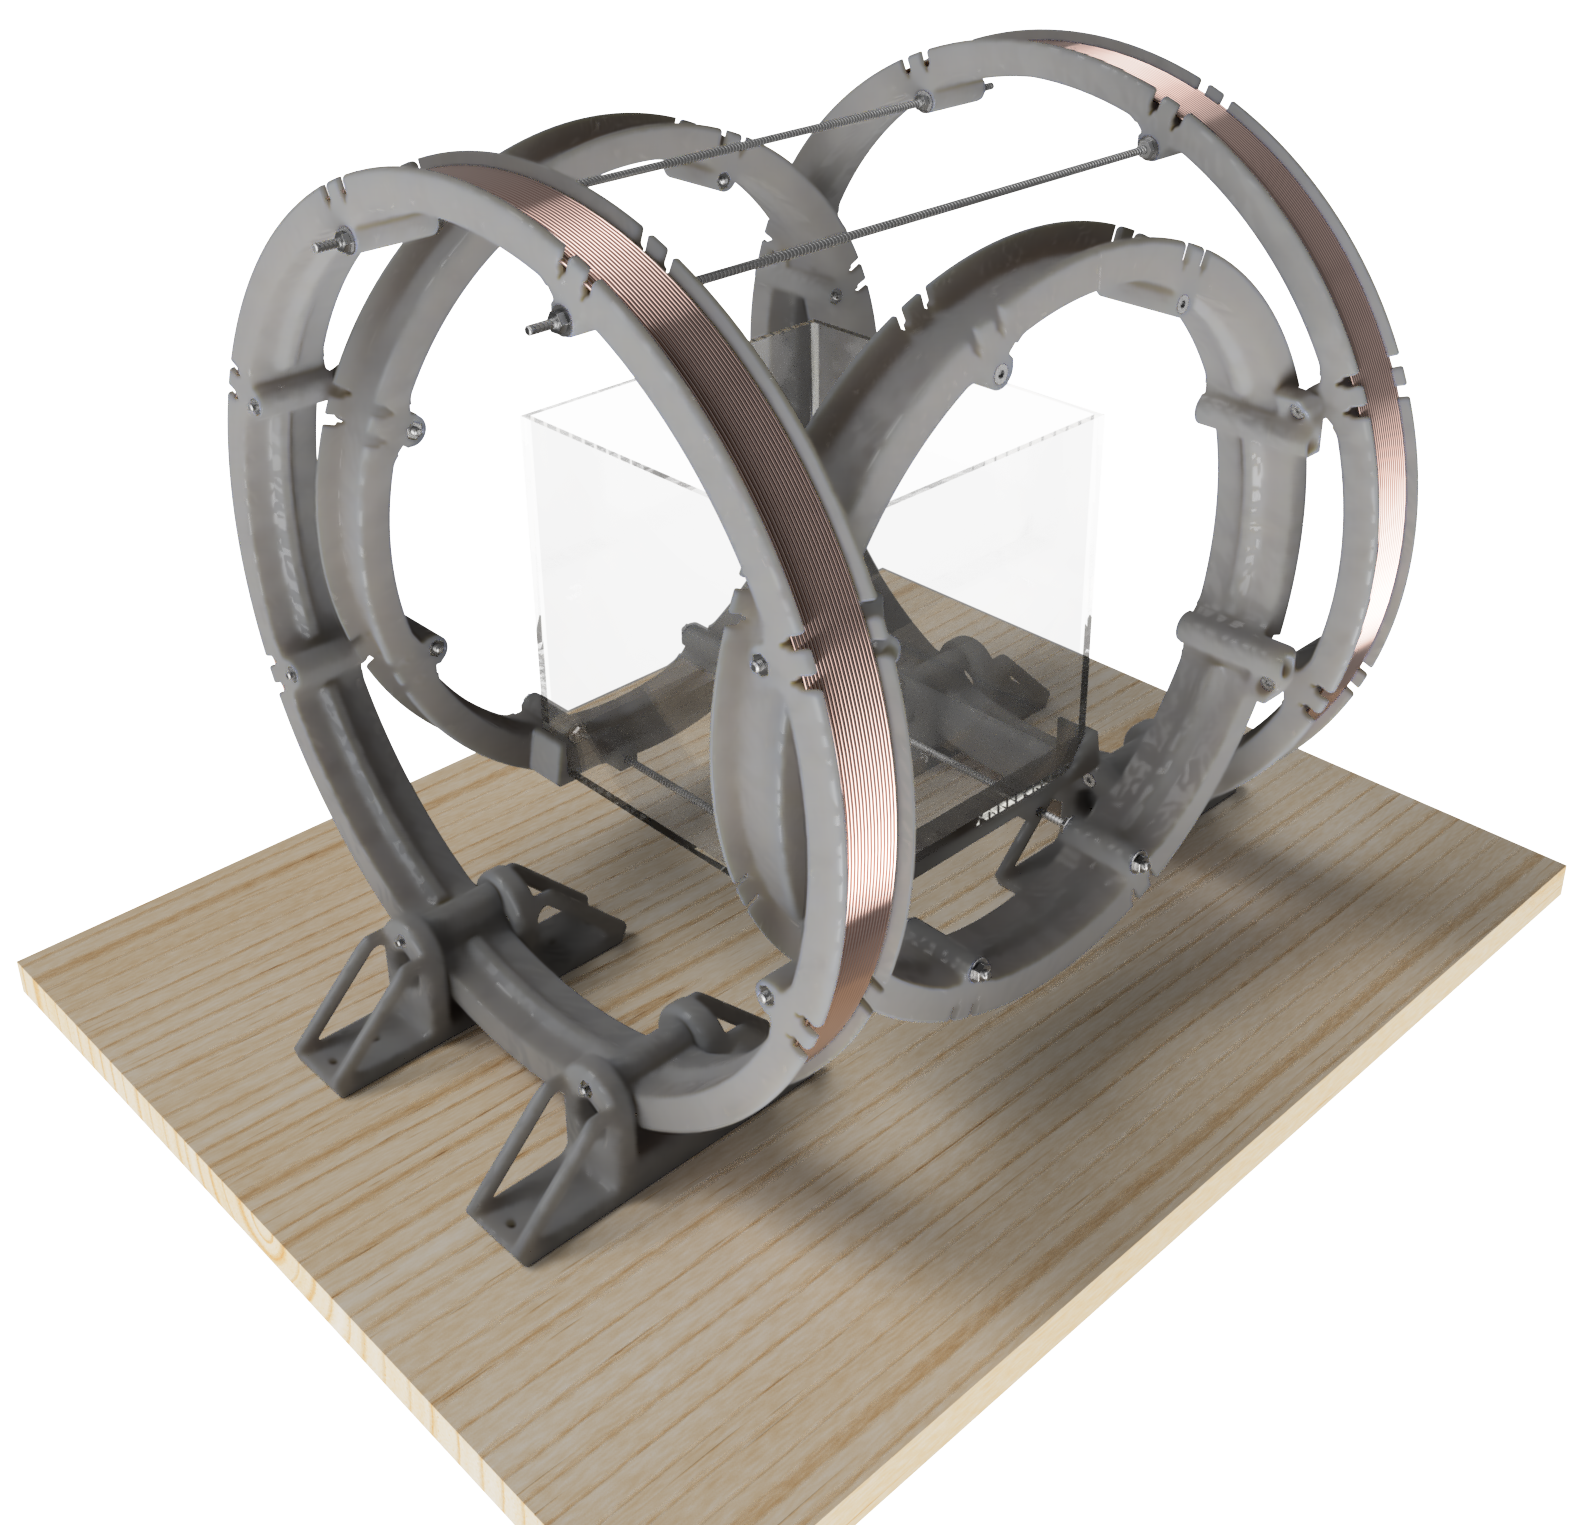
\includegraphics[width = 0.65\textwidth]{Images/Proto2.PNG}
            \caption{Plan 3D Solidworks du deuxième système envisagé.}
            \label{fig:sytèmeV2}
        \end{figure}
\noindent
Ce système est facilement réalisable, car toutes les pièces grises sont conçues pour être imprimées en 3D séparément et assemblées par simple clipsage et vissage. Par exemple, un support de bobine est constitué de huit pièces assemblables afin de s'adapter à la zone imprimable et d'éliminer les surplombs et les supports d'impression. Les jeux nécessaires à une bonne imbrication ont été pris en compte. La seule étape un peu technique et fastidieuse est le bobinage du cuivre.
\begin{figure}[H]
        \centering
            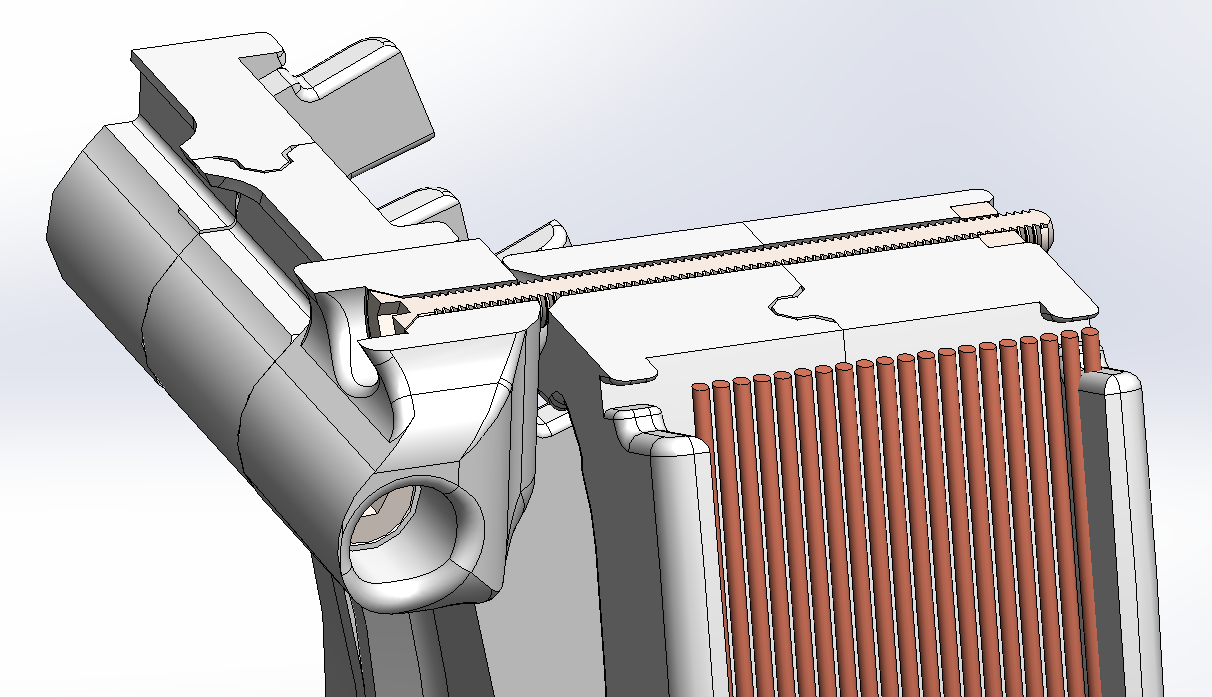
\includegraphics[width = 0.5\textwidth]{Images/coupe_proto2.png}
            \caption{Visualisation du système de jonction des pièces envisagé.}
            \label{fig:sytèmeV2_img2}
        \end{figure}
\noindent
Une de ces pièces a d'ailleurs été imprimée pour vérifier le bon emboîtement.\\
Avant de lancer les impressions 3D complètes, un petit prototype simplifié de ce système a été réalisé rapidement. Deux bobines identiques ont été fabriquées à la main, accompagnées d'un petit récipient pour l'eau.
\begin{figure}[H]
    \centering
    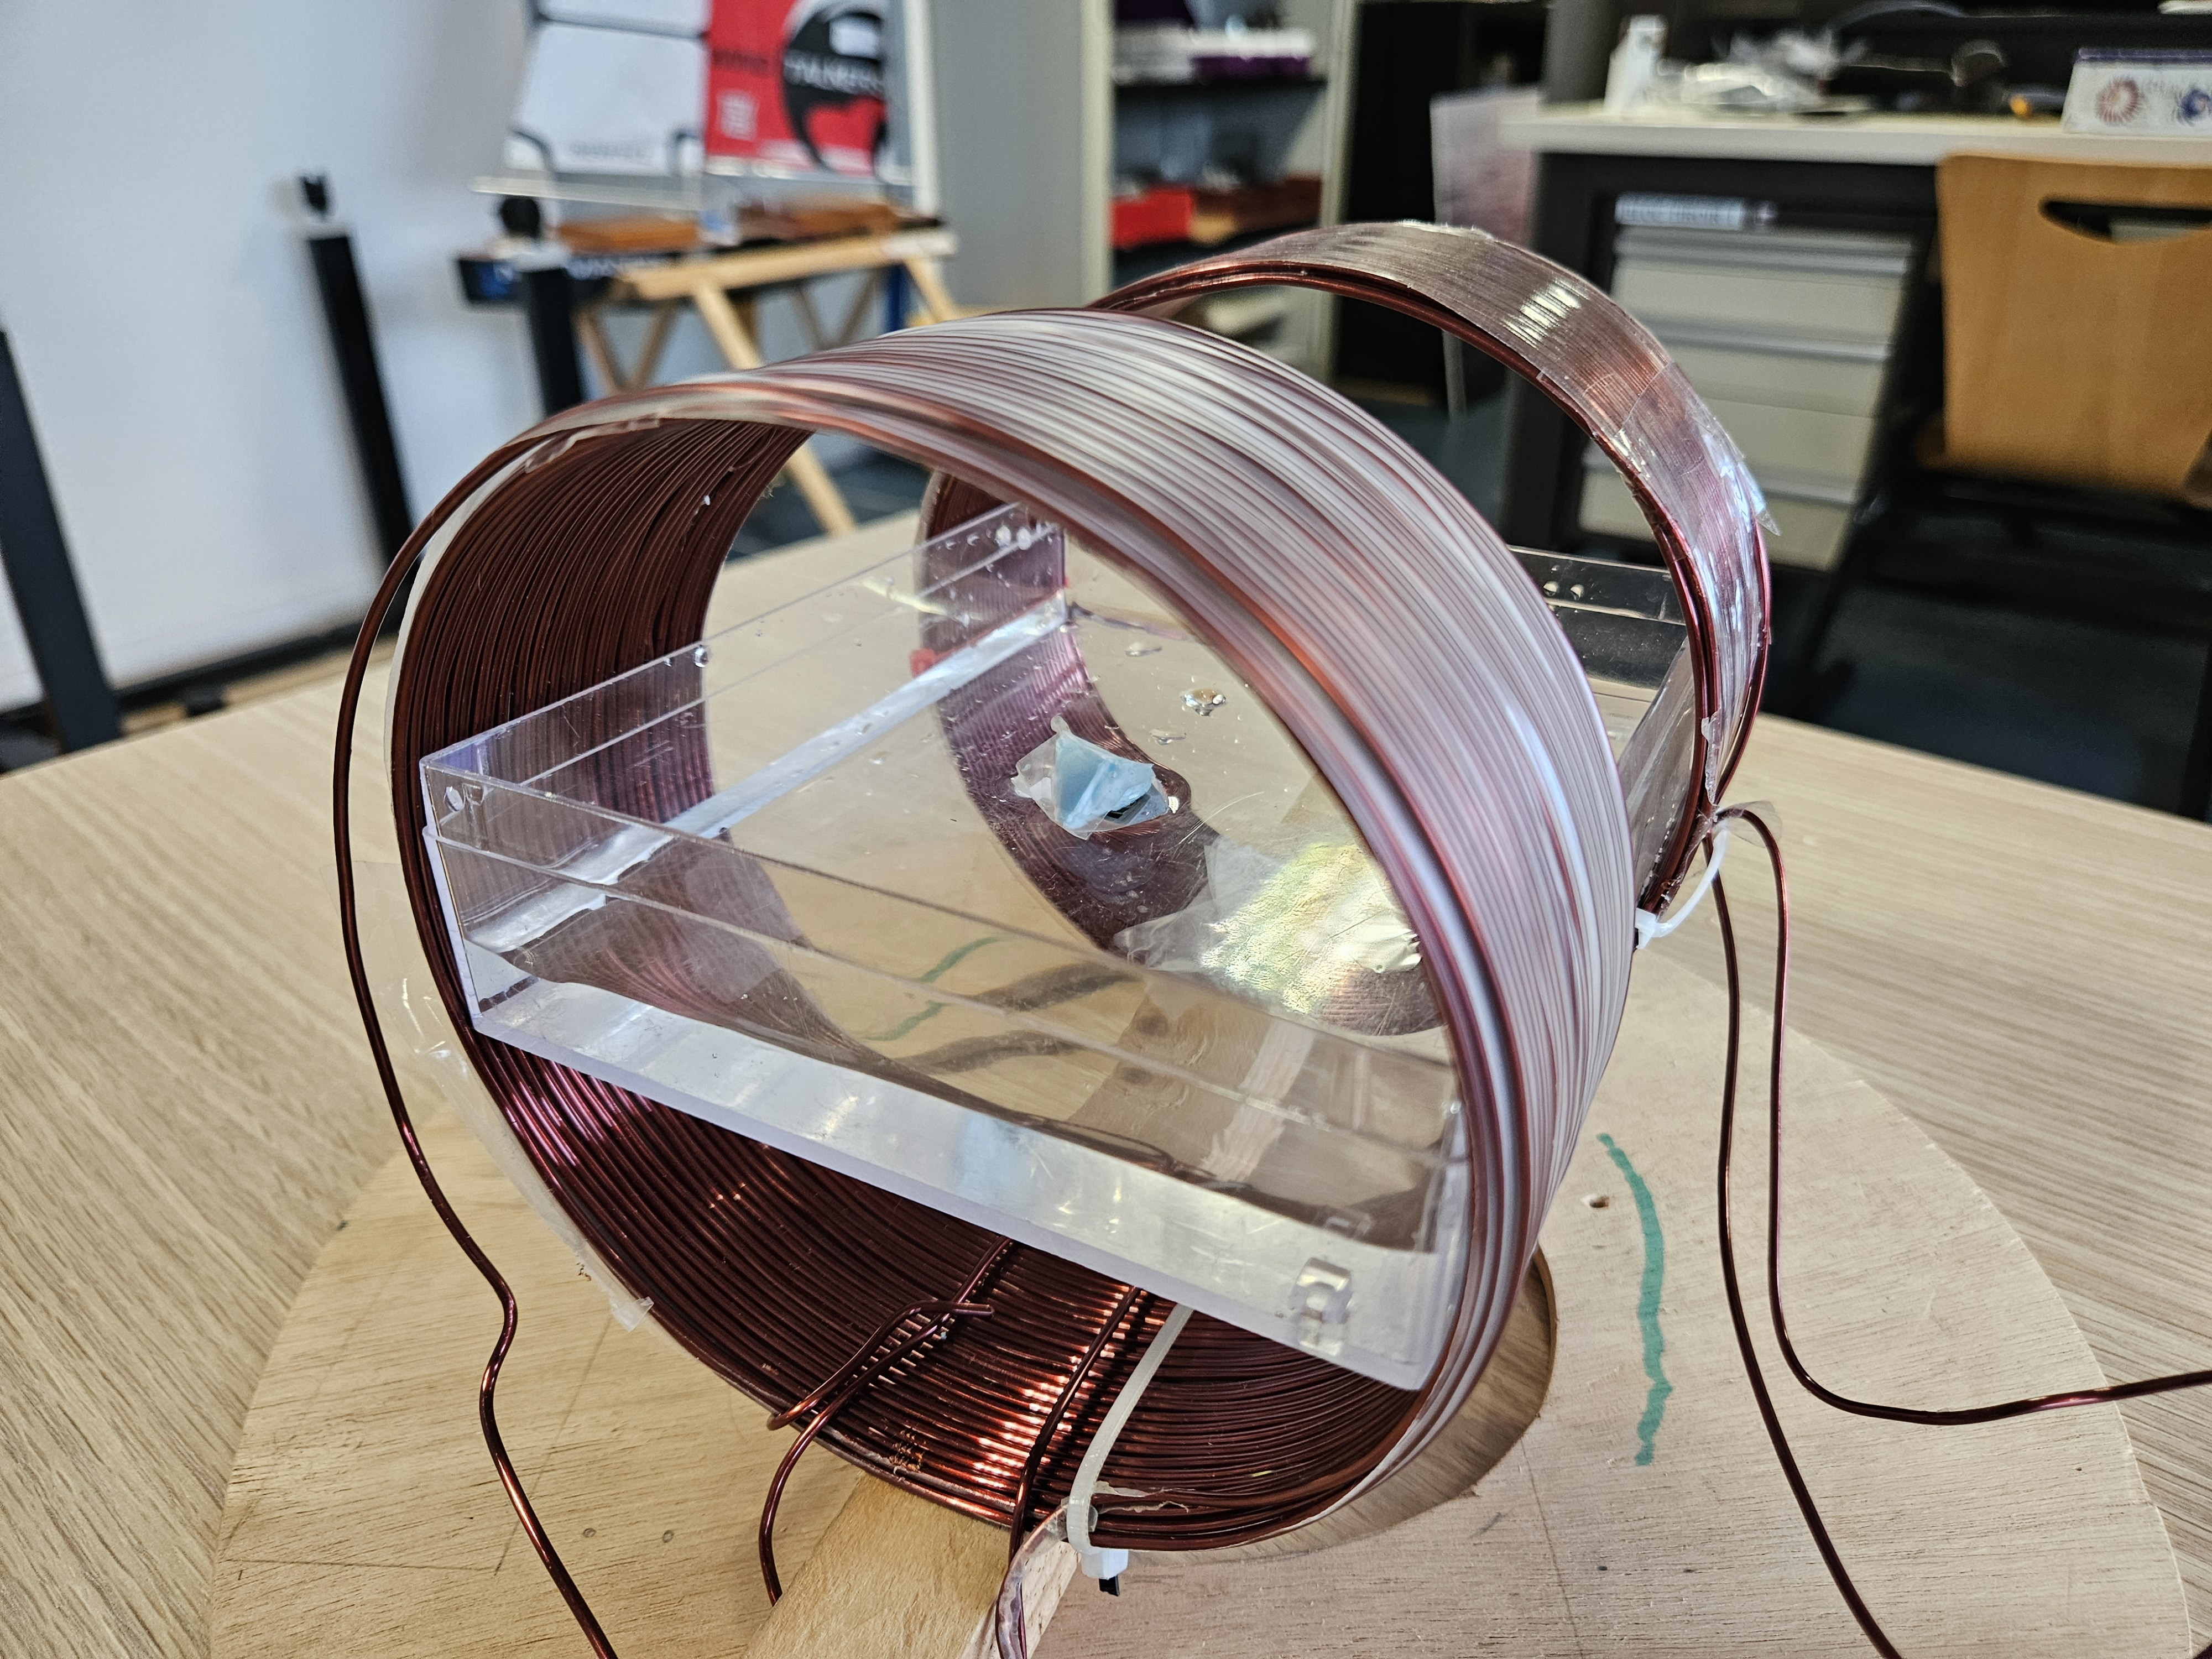
\includegraphics[width=0.5\linewidth]{Images/proto_test_1.jpg}
    \caption{Photographie du prototype réalisé}
    \label{fig:proto_test_1}
\end{figure}
\noindent
Cela a confirmé les problèmes décrits dans la section précédente. Cependant, le déplacement de l'aimant sur un seul axe fonctionnait bien. Un simple circuit électronique contenant deux commutateurs permettait d'allumer l'une ou l'autre des bobines. En revanche, la zone de travail était d'environ 10 cm, ce qui est un peu restreint.

\subsection{Révision de nos acquis et recherche d'un système plus fiable}

Le 7 mars, une réunion avec notre professeur référent a été organisée. Après avoir exposé nos démarches et présenté notre prototype, il a souligné un aspect crucial. Bien que le système envisagé aurait probablement fonctionné, il présentait une zone de travail restreinte (15 cm x 15 cm). De plus, l'utilisation de grandes bobines créait un champ magnétique sur une section étendue de l'espace, entraînant une dissipation d'énergie inutile. Étant donné que le microrobot évolue uniquement dans un plan, l'utilisation de bobines plus petites avec un nombre de tours plus élevé est une option plus judicieuse. En plus, des bobines de ce type étaient déjà disponibles à l'ISEN.
\\
\\
Malgré le travail déjà fourni pour la version précédente du système, il a été choisi de changer complètement la configuration. En effet, suite à la suggestion de notre professeur et aux avantages techniques de son idée, un système basé sur 8 "petites" bobines identiques réparties en octogone a été privilégié.
\\
\\
Pour simplifier la compréhension du fonctionnement du système, envisageons qu'une seule bobine soit activée à la fois, attirant ainsi le microrobot vers elle. 
\begin{figure}[H]
    \centering
    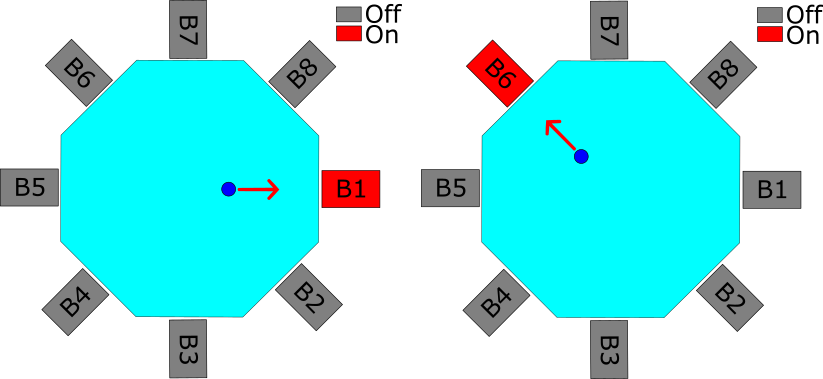
\includegraphics[width=0.5\linewidth]{Images/Explication_simple.png}
    \caption{Schéma simplifié du système à 8 bobines. Le point bleu foncé représente le microrobot magnétique.}
    \label{fig:Schéma_simplifié}
\end{figure}
\noindent
Cependant, des complications subsistent. Notamment, les gradients de champ magnétique ne seront pas uniformes, ce qui entraînera une augmentation significative de la force magnétique à mesure que le microrobot se rapproche d'une bobine. Il faudra également combiner des champs magnétique pour optimiser les mouvements du microrobot et atténuer certains effets indésirables.

\subsection{Détermination de l'intensité du champ nécessaire à la propulsion du microrobot}

Pour déterminer la distance maximale à laquelle le microrobot peut être déplacé, il est nécessaire de prendre en compte la force qui lui sera appliquée par le champ magnétique et la force de frottement due à l'eau. L'objectif visé est d'obtenir une zone de travail étendue, approximativement de 30 à 50 centimètres, permettant au microrobot de la traverser dans un laps de temps raisonnable, inférieur à 5 secondes.
\\
 Les aimants disponibles sont des cubes de 5 mm de côté.
\begin{figure}[H]
    \centering
    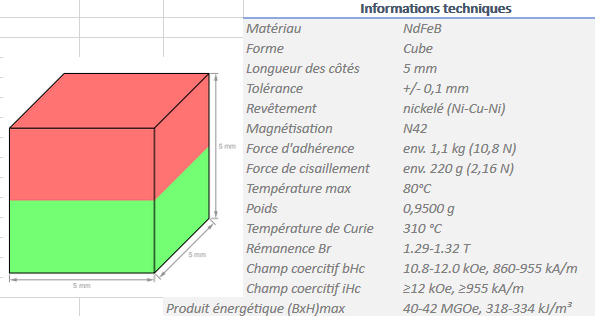
\includegraphics[width=0.5\linewidth]{Images/info_aimant.png}
    \caption{Informations techniques sur les aimants utilisés.}
    \label{fig:info_aimants}
\end{figure}
\subsubsection{Force hydrodynamique}
Dans un premier temps, pour simplifier les calculs et permettre au microrobot de s'orienter librement dans le champ magnétique, il est préférable d'utiliser un microrobot sphérique. En effet, les calculs hydrodynamiques pour une sphère sont plus simples.
\\
\\
Pour créer une sphère flottante complètement étanche, une solution relativement simple consiste à imprimer une sphère creuse avec un support central pour l'aimant. Pour la rendre étanche, il suffit d'ajouter une pause au milieu de l'impression, d'y coller l'aimant, puis de relancer l'impression. Ensuite, pour combler d'éventuelles porosités du plastique, il est possible d'ajouter une fine couche de peinture époxy ou de polyuréthane d'une couleur reconnaissable pour la caméra (voir la section \ref{Système de commande informatique}). 
\\
\\
Pour déterminer la taille de la sphère, un simple calcul d'Archimède peut être utilisé.
Pour que les deux aimants tiennent dans la sphère, il leur faut un support, une simple extrusion partant du bas de la sphère vers le haut avec une cavité pour ranger l'aimant suffit. Un trou en forme d'hexagone est percé à l'intérieur pour réduire la masse et éviter des supports d'impression. Le volume de cette pièce sera appelé $V_{\text{support}}$ et sera déterminé avec SolidWorks.

\begin{figure}[H]
    \centering
    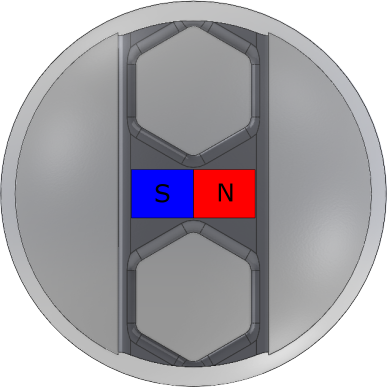
\includegraphics[width=0.25\linewidth]{Images/shema_sphere.png}
    \caption{Vue intérieure de la sphère contenant les aimants}
    \label{fig:shéma_sphère}
\end{figure}
\noindent
Pour déterminer le rayon \( R_{\text{Sphère}} \), il faut utiliser les formules et hypothèses suivantes :
\\
\\
L'épaisseur des parois est de 3 fois l'épaisseur de la buse d'impression, soit  $Ep = 1.2 \times 10^{-3}\, \text{m}$ \\\\
$P_{\text{Archimède}} = \rho_{\text{Eau}} \cdot \frac{4}{3} \cdot \pi \cdot R_{\text{Sphère}}^3 \cdot g$ \\\\
$P_{\text{Sphère}} = g \cdot (\frac{4}{3} \cdot \pi \cdot \rho_{\text{PLA}}\cdot (R_{\text{Sphère}}^3  - (R_{\text{Sphère}}-Ep)^3)  +  m_{\text{Peinture}} + 2 \cdot m_{\text{Aimant}}+\rho_{\text{PLA}} \cdot V_{\text{support}} )$ \\\\
Considérons que la sphère est semi-enfouie dans l'eau, il faut que $2 \cdot P_{\text{Sphère}} = P_{\text{Archimède}}$ 
\\
\\
En utilisant les valeurs :
\begin{align*}
    & m_{\text{Aimant}} = 0.95 \times 10^{-3}\, \text{Kg} \\
    & m_{\text{Peinture}} = 1\times 10^{-3}\, \text{Kg} \\
    & \rho_{\text{PLA}} = 1250\, \text{Kg}\cdot \text{m}^{-3} \\
    & \rho_{\text{Eau}} = 1000\, \text{Kg}\cdot \text{m}^{-3} \\
    & V_{\text{support}} = 9.823 \times 10^{-7}\, \text{m}^{3} \\
    & g = 9.81\, \text{m}\cdot {s}^{-2}
\end{align*}
Il vient, par une résolution graphique :
\[ R_{\text{Sphère}} = 16\, \text{mm} \]
\[ m_{\text{Sphère}} = 8.6\, \text{g} \]
\noindent
Maintenant, il est possible de déterminer la force à appliquer à cette sphère pour la faire parcourir une distance $d$ en $x$ secondes.\\\\Pour commencer, il faut déterminer la force de traînée de la sphère. Selon \cite{ref7}, la formule varie en fonction du nombre de Reynolds ($R_{\text{e}}$) de l'écoulement. Si $R_{\text{e}}< 1$, alors l'écoulement est laminaire et la formule applicable est $F = K\cdot \nu_{\text{itesse}}$. Par contre, si $R_{\text{e}}> 1$, l'écoulement est turbulent, ce qui nécessite l'utilisation de la formule $F= \frac{1}{2}\cdot \rho_{\text{eau}}\cdot \nu_{\text{itesse}}^2\cdot C_x\cdot S_{\text{urface}}$.
\\\\
Ce nombre est déterminé pour une sphère par $R_{\text{e}} = \frac{\nu_{\text{itesse}} \cdot D_{\text{iamètre}}}{\eta}$ avec $\eta$ la viscosité cinématique de l'eau ($1 \times 10^{-6} \, \text{m}^2/\text{s}$). En se basant sur les objectifs définis au début de la section, il est raisonnable d'estimer que la vitesse sera inférieure à 10 km/h, ce qui donne $R_{\text{e}} \in [10000:100000]$.
\\
\\
Le coefficient de traînée $C_x$ d'une sphère peut être déterminé à l'aide de ce graphique :

\begin{figure}[H]
    \centering
    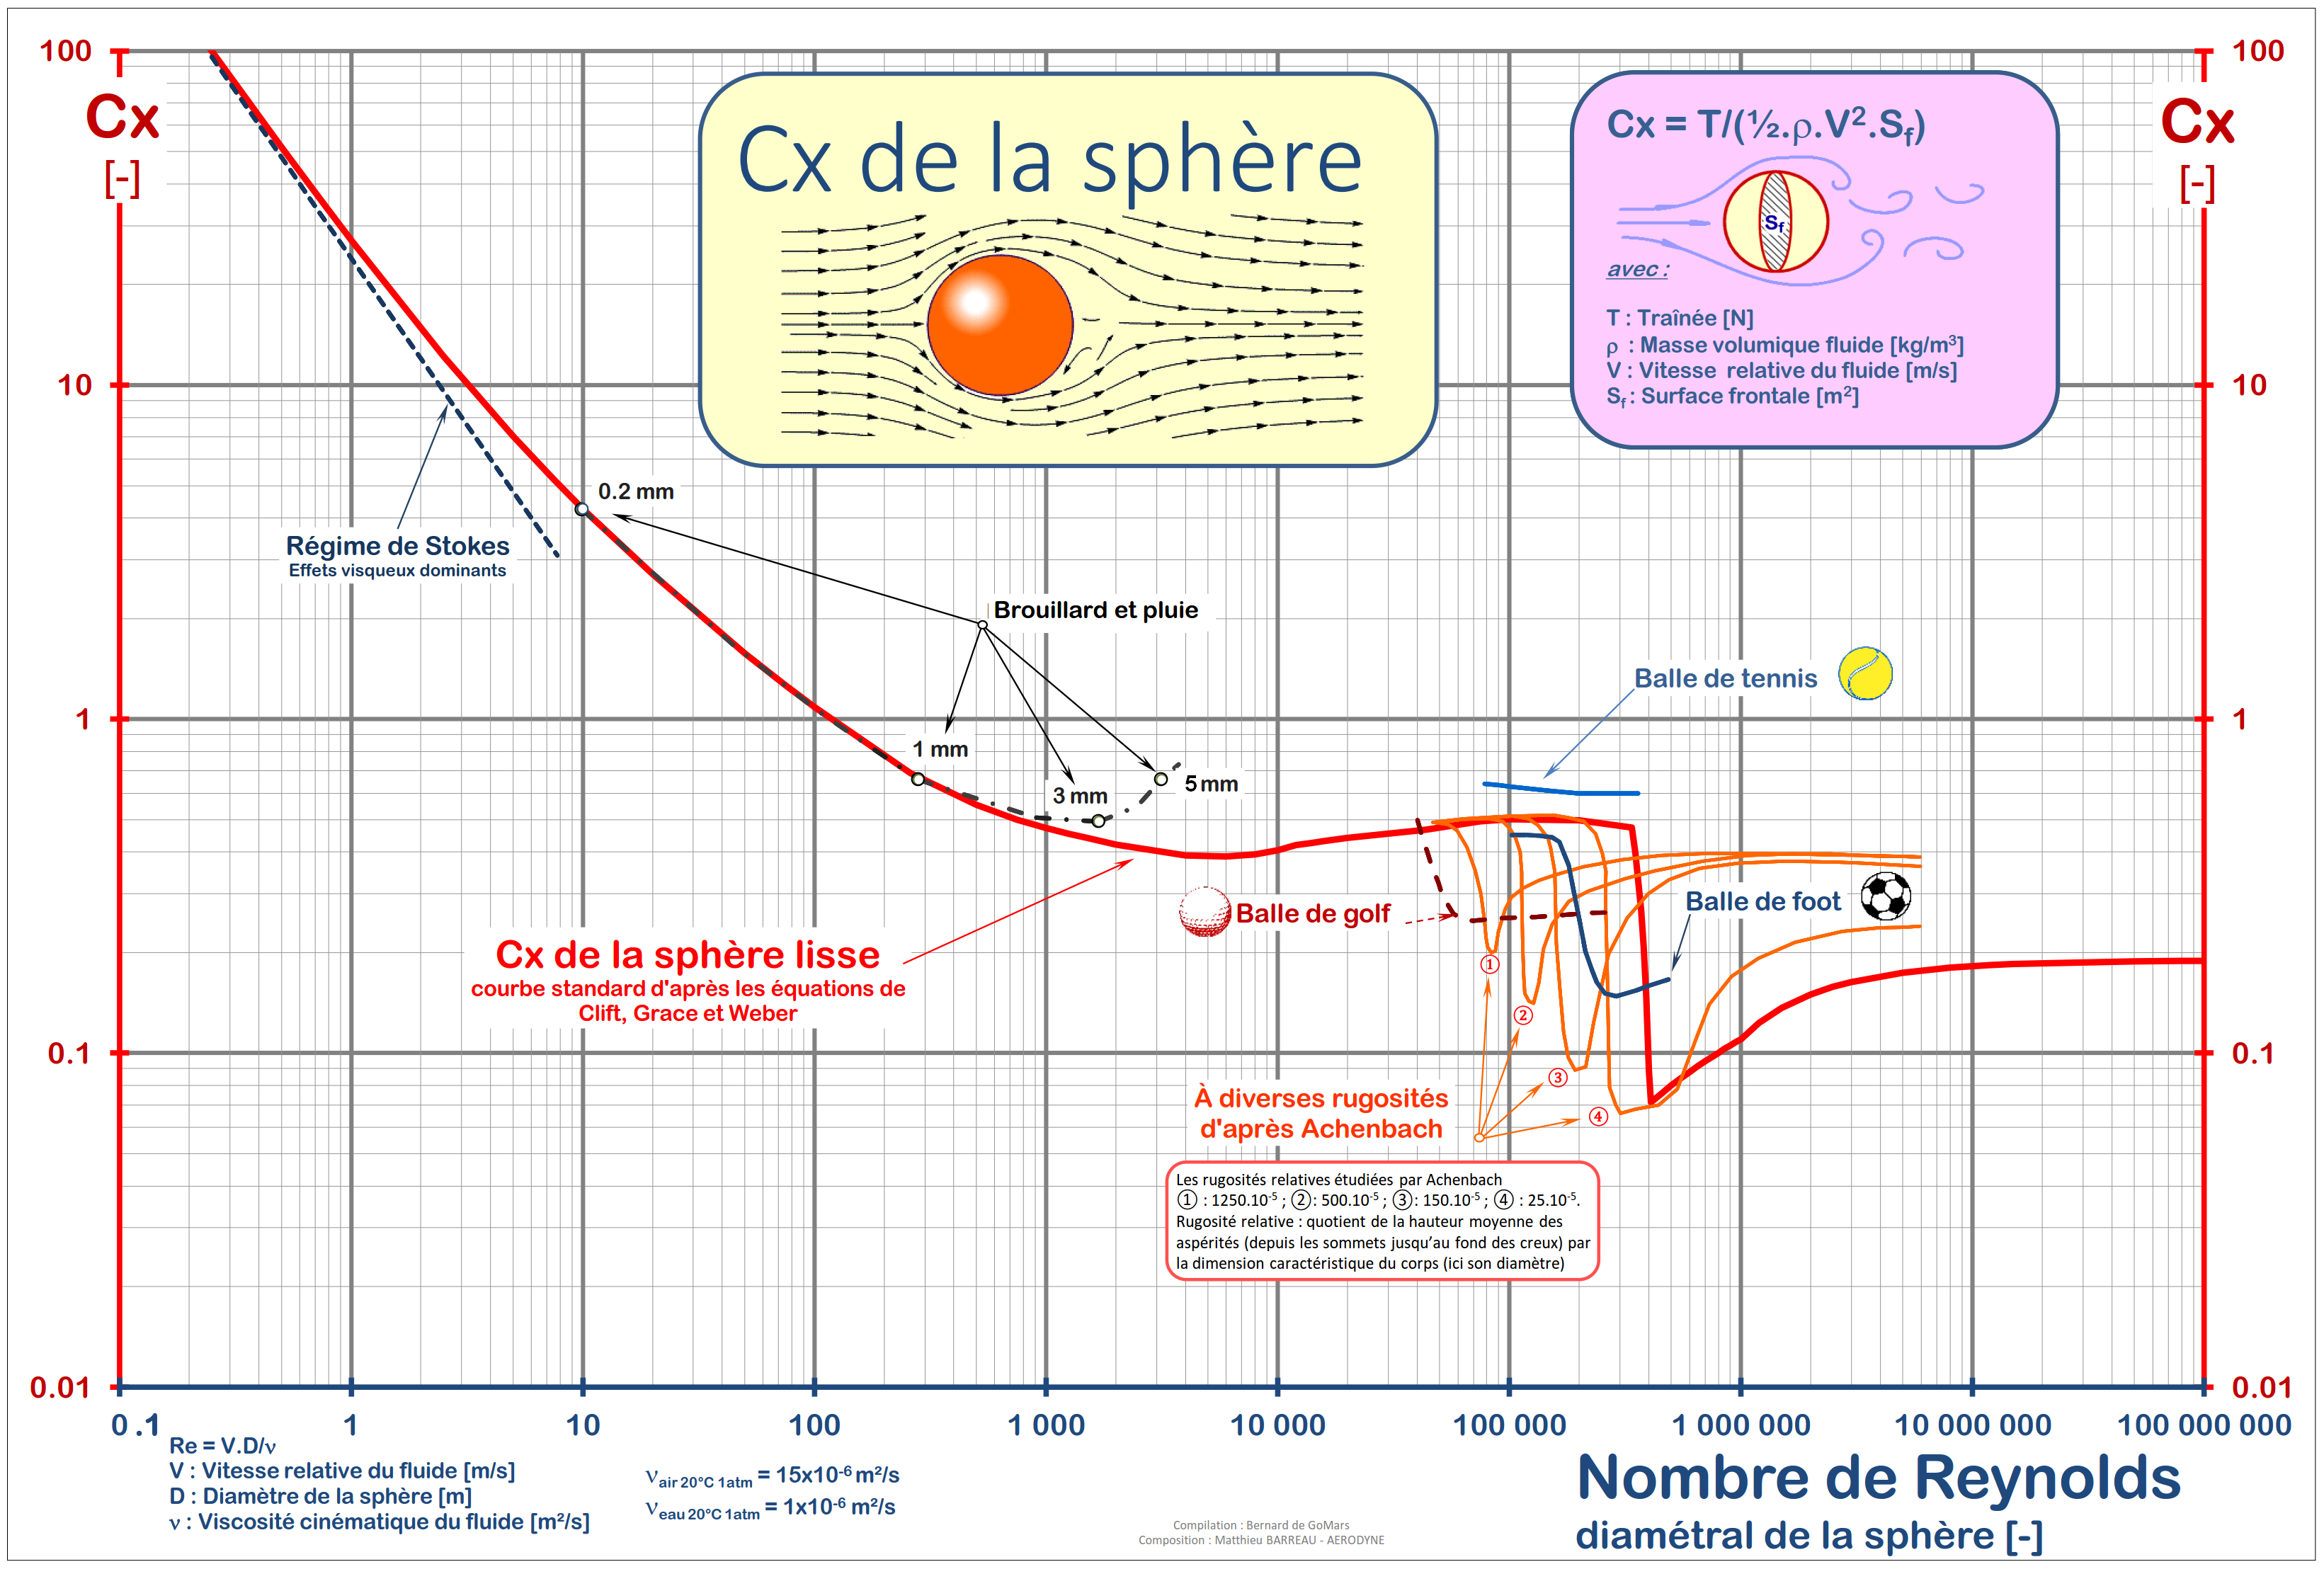
\includegraphics[width=0.7\linewidth]{Images/CX_SPHERE.png}
    \caption{Cx de la sphère \cite{ref7} (Par Bernard de Go Mars — Travail personnel, CC BY-SA 4.0)}
    \label{fig:Cx_sphere}
\end{figure}
\noindent
Dans l'intervalle de Reynolds choisi, $C_x \approx 0.5$ .
\\
La force de frottement dans l'eau est donc calculable en utilisant la formule pour l'écoulement turbulent :
\begin{equation}
F_{\text{Eau}} = \frac{1}{2} \cdot \rho_{\text{eau}} \cdot \nu_{\text{itesse}}^2 \cdot C_x \cdot S_{\text{urface}}
\end{equation}
Avec la deuxième loi de Newton : $F_{\text{déplacement}} - F_{\text{Eau}} = m \cdot a$, en posant l'accélération $a = \frac{2z}{t^2}$ et $\nu_{\text{itesse}} = a \cdot t$, il vient:
\begin{equation}
\begin{aligned}
F_{\text{déplacement}} &= m\left(\frac{2z}{t^2}\right) + \frac{1}{2} \cdot \rho \cdot \left(\frac{2z}{t}\right)^2 \cdot C_x \cdot S_{\text{urface}} \\
&= \frac{2z}{t^2} \cdot \left(m + \rho \cdot C_x \cdot S_{\text{urface}} \cdot z\right)
\end{aligned}
\label{eq:EquationMagEau}
\end{equation}
Cette équation décrit le profil de la force à appliquer sur la sphère en fonction de la distance à laquelle elle se situe de son point d'arrivée (0m).\\\\Si on la trace, on obtient une courbe du second degré :
\begin{figure}[H]
        \centering
        \begin{tikzpicture}
            \begin{axis}[
                axis lines = left,
                xlabel = \(z\) (m),
                ylabel = {\(\mathbf{F_{\text{déplacement}}}(z)\) (N)},
                legend pos = north east,
            ]
            % Below the red parabola is defined
            \addplot [
                domain=0:0.5, 
                samples=100, 
                color=red,
            ]
            {((2*x)/25)*(0.0086+1000*0.5*0.0004*x)};
            \end{axis}
        \end{tikzpicture}
                            \caption{Courbe de la force à appliquer sur le microdrone pour le déplacer à vitesse constante.}
            \label{fig:courbe_force0}
\end{figure}
\noindent
Avec les objectifs précédents, pour déplacer la sphère sur un bassin de 30 à 50 cm, une force maximale entre 0.0016 N et 0.0043 N serait nécessaire. Ensuite, pour avancer à une vitesse constante, il est nécessaire de réduire progressivement la force en suivant le profil de la courbe. 
\\
La prochaine étape consiste à étudier le profil de la force du champ magnétique (son gradient) appliqué sur le microrobot à une distance \( z \) de la bobine.
\\
\\
\subsubsection{Force électromagnétique générée par une bobine}
Comme vu dans l'eqation \ref{eq:ForceMag} la force appliquer sur un dipole par un champ magnetique est determinable. Elle depend du moment magnetique de l'aimant contenue dans le microrobot et du gradient du champ magnétique dans lequel il est plongée. 
\\
\\
Le moment magnétique de l'aimant est donné par $\mu = \mathcal{M}\cdot V_{\text{Aimant}}$, avec $\mathcal{M}$ l'aimantation en $A/m$ et $V_{\text{Aimant}}$ le volume de l'aimant. Ici, $\mu = 0.12 \, A.m^2$.
\\
\\
En réutilisant l'équation \ref{eq:Equation2} avec les paramètres des nouvelles bobines et en appliquant l'équation de force \ref{eq:ForceMag}, il est possible de tracer la courbe de la force appliquée sur l'aimant en fonction de la distance $z$.
\begin{figure}[H]
        \centering
        \begin{tikzpicture}
            \begin{axis}[
                axis lines = left,
                xlabel = \(z\) (m),
                ylabel = {\(\mathbf{F}(z)\) (N)},
                legend pos = north east,
            ]
            % Below the red parabola is defined
            \addplot [
                domain=0:0.5, 
                samples=100, 
                color=green,
            ]
            {0.12*((0.000001884*x)/((0.0025+x^(2))^(((5)/(2)))))};
            \addlegendentry{\(R=50 \, \text{mm}, I=8 \, \text{A} , n=500\)}
            \end{axis}
        \end{tikzpicture}
                    \caption{Courbe de la force appliquée sur le microdrone par le gradient magnétique.}
            \label{fig:courbe_force}
\end{figure}
\noindent
Il est clair que la force devient pratiquement nulle au-delà d'une distance de 0.2 m. Comme expliqué précédemment, la force nécessaire pour déplacer le microrobot en un temps de 5 secondes sur une distance de 0.3 à 0.5 mètres est entre 0.0016 N et 0.0043 N.
\\\\
Il n'est donc pas possible d'avoir un bassin de 30 a 50 cm de long en utilisant simplement les bobines récuperer.
\\\\
Une solution pour augmenter l'intensité du champ magnétique consiste à insérer un matériau ferromagnétique au centre de la bobine, tel un électroaimant. Des matériaux comme de l'acier ou, mieux encore, du fer doux ont une perméabilité relative beaucoup plus importante que l'air, ce qui a pour effet de canaliser les lignes de champ magnétique.
\\\\
Pour calculer la force que cette configuration pourra produire, les calculs deviennent considérablement plus complexes. Une solution envisagée est de considérer la bobine et le matériau ferromagnétique comme un électroaimant, formant ainsi un seul dipôle. Cette approche est similaire à celle d'un gros aimant permanent contrôlable. Ensuite, on peut calculer la force d'attraction entre l'électroaimant et le petit aimant du microrobot.
\\\\
Après avoir consulté notre professeur référent, celui-ci nous a indiqué que cette approche devrait fonctionner, mais que pour plus de précision, il serait judicieux de considérer l'électroaimant comme un assemblage de plusieurs dipôles et de sommer leurs effets, comme expliqué dans sa thèse \cite{ref8}. Le logiciel de simulation Ansys Maxwell est utilisé pour fournir une précision supplémentaire.
\begin{figure}[H]
    \centering
    \begin{minipage}{0.45\textwidth}
        \centering
        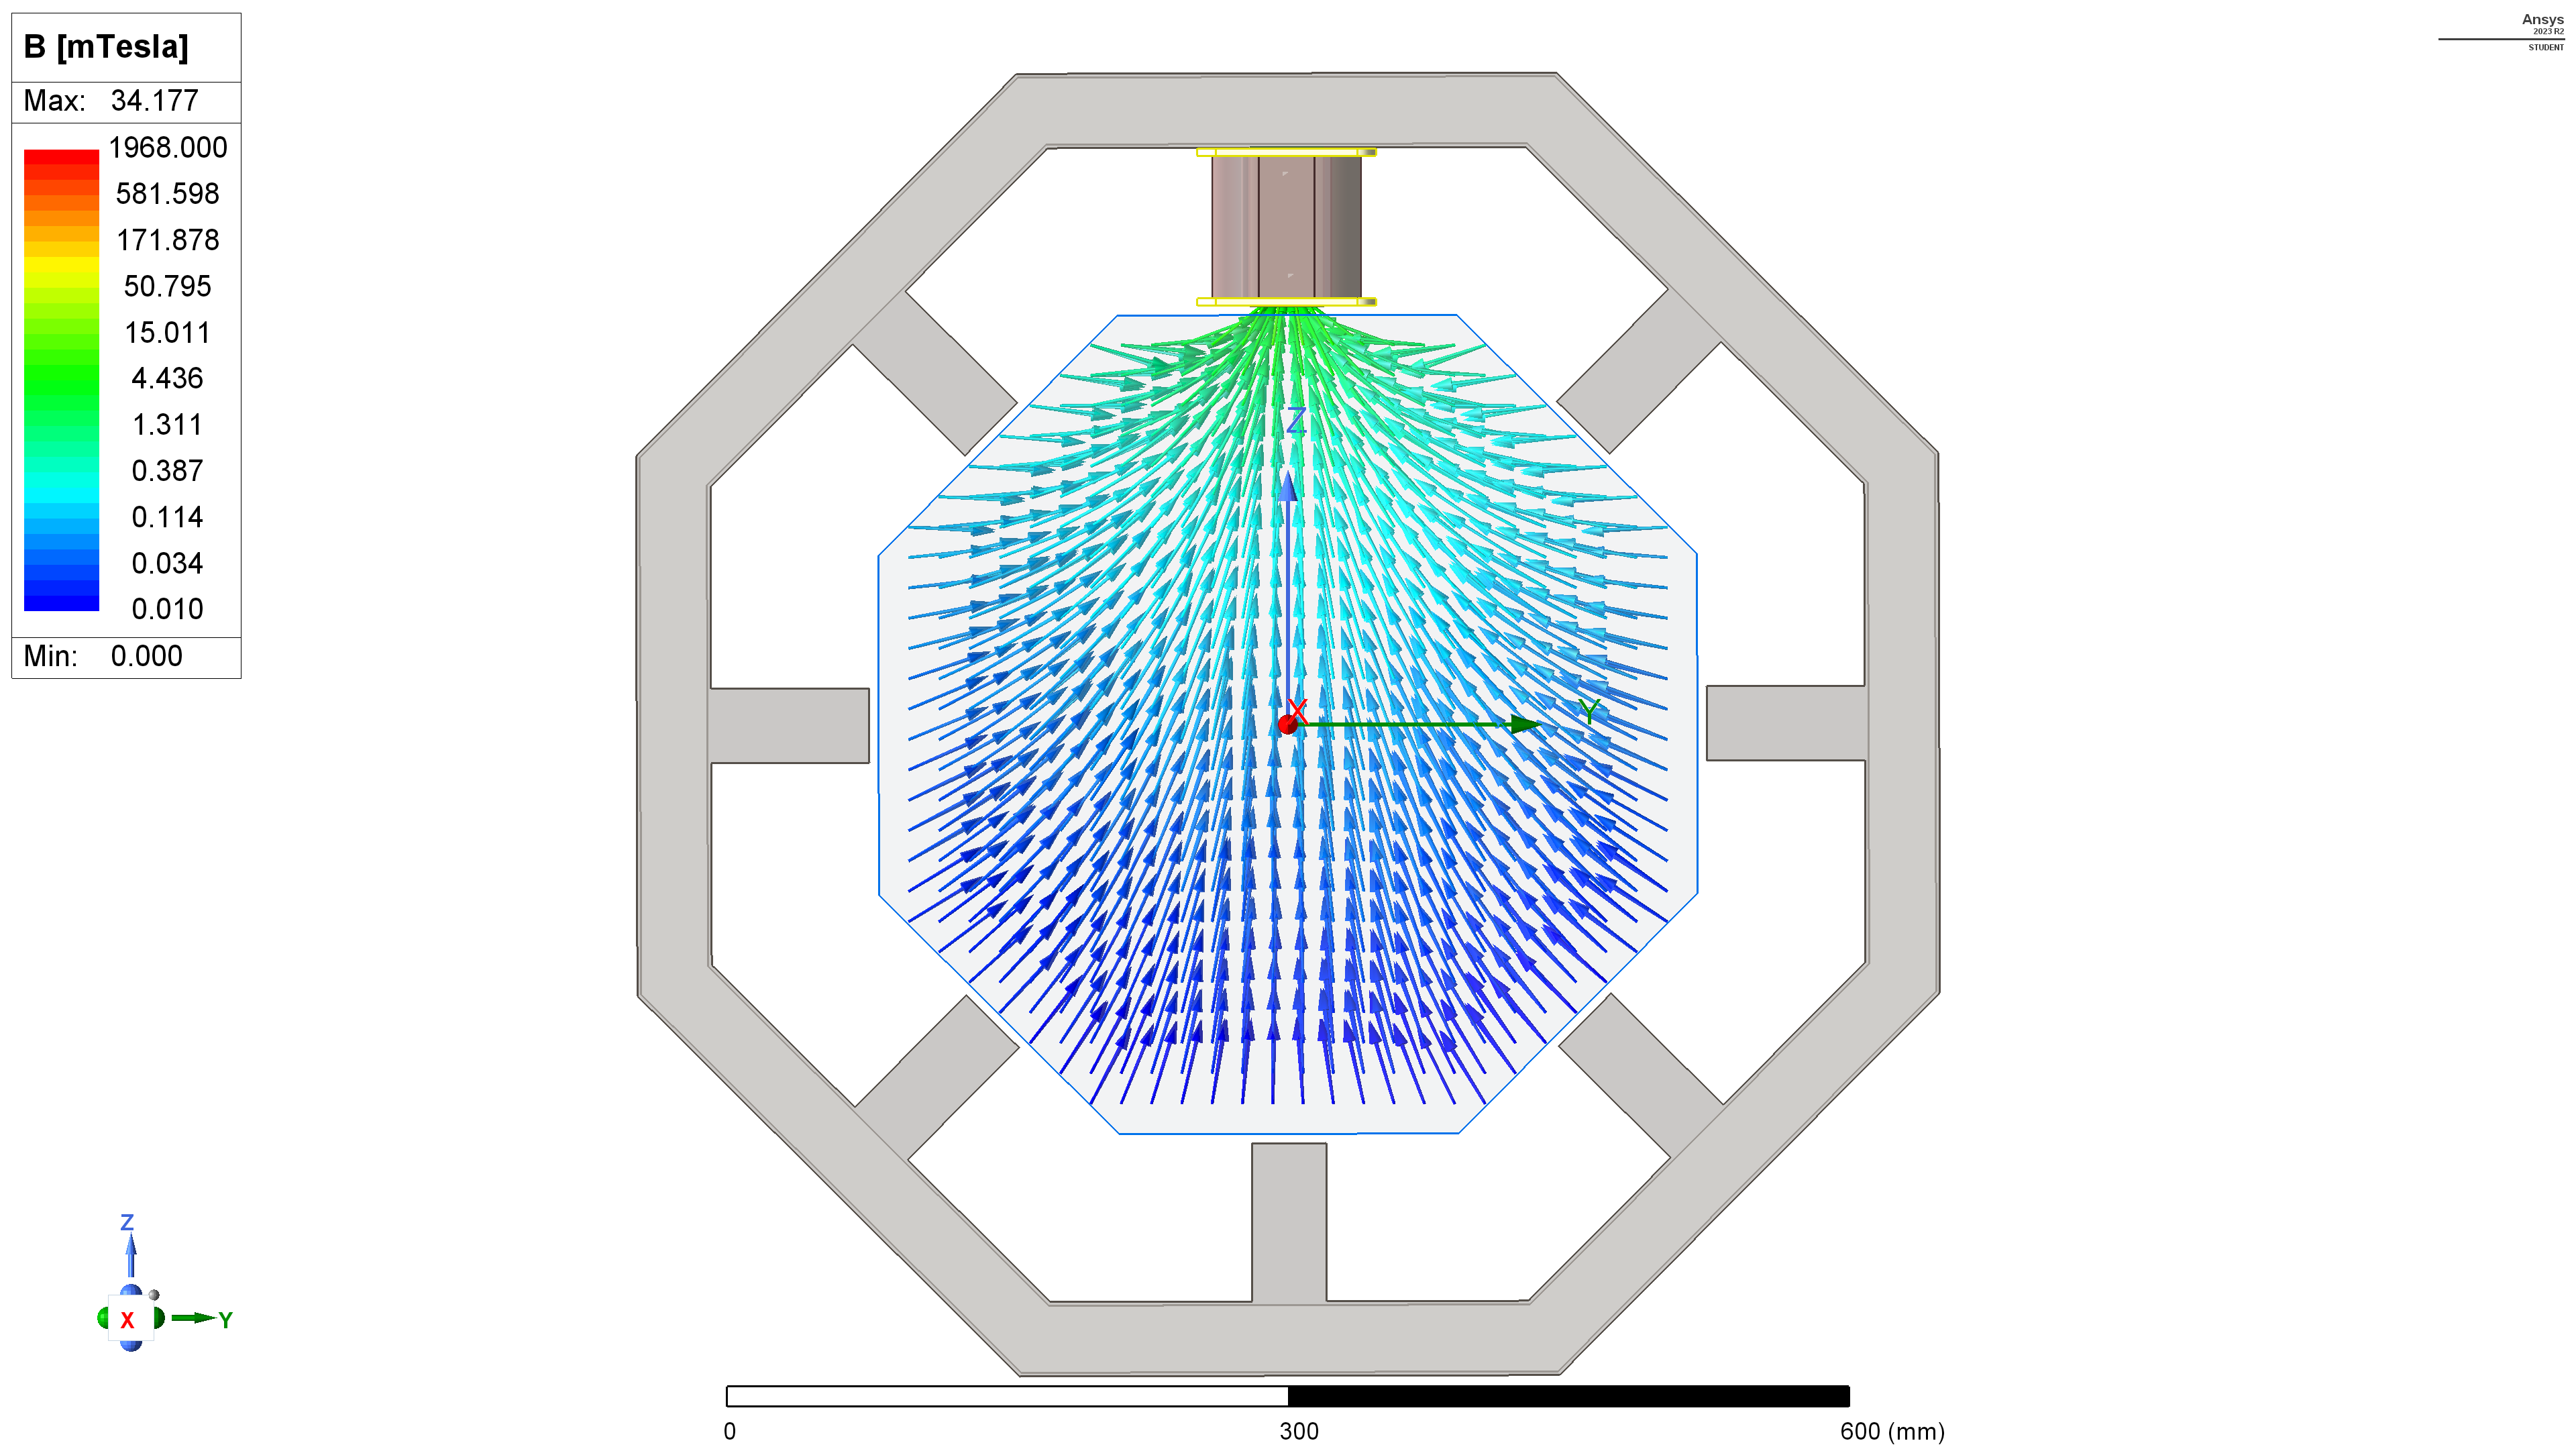
\includegraphics[width=\linewidth]{Images/SupportPlastique.png}
        \caption{Visualisation des lignes du champ magnétique d'une bobine sans cœur ferromagnétique.}
    \end{minipage}\hfill
    \begin{minipage}{0.45\textwidth}
        \centering
        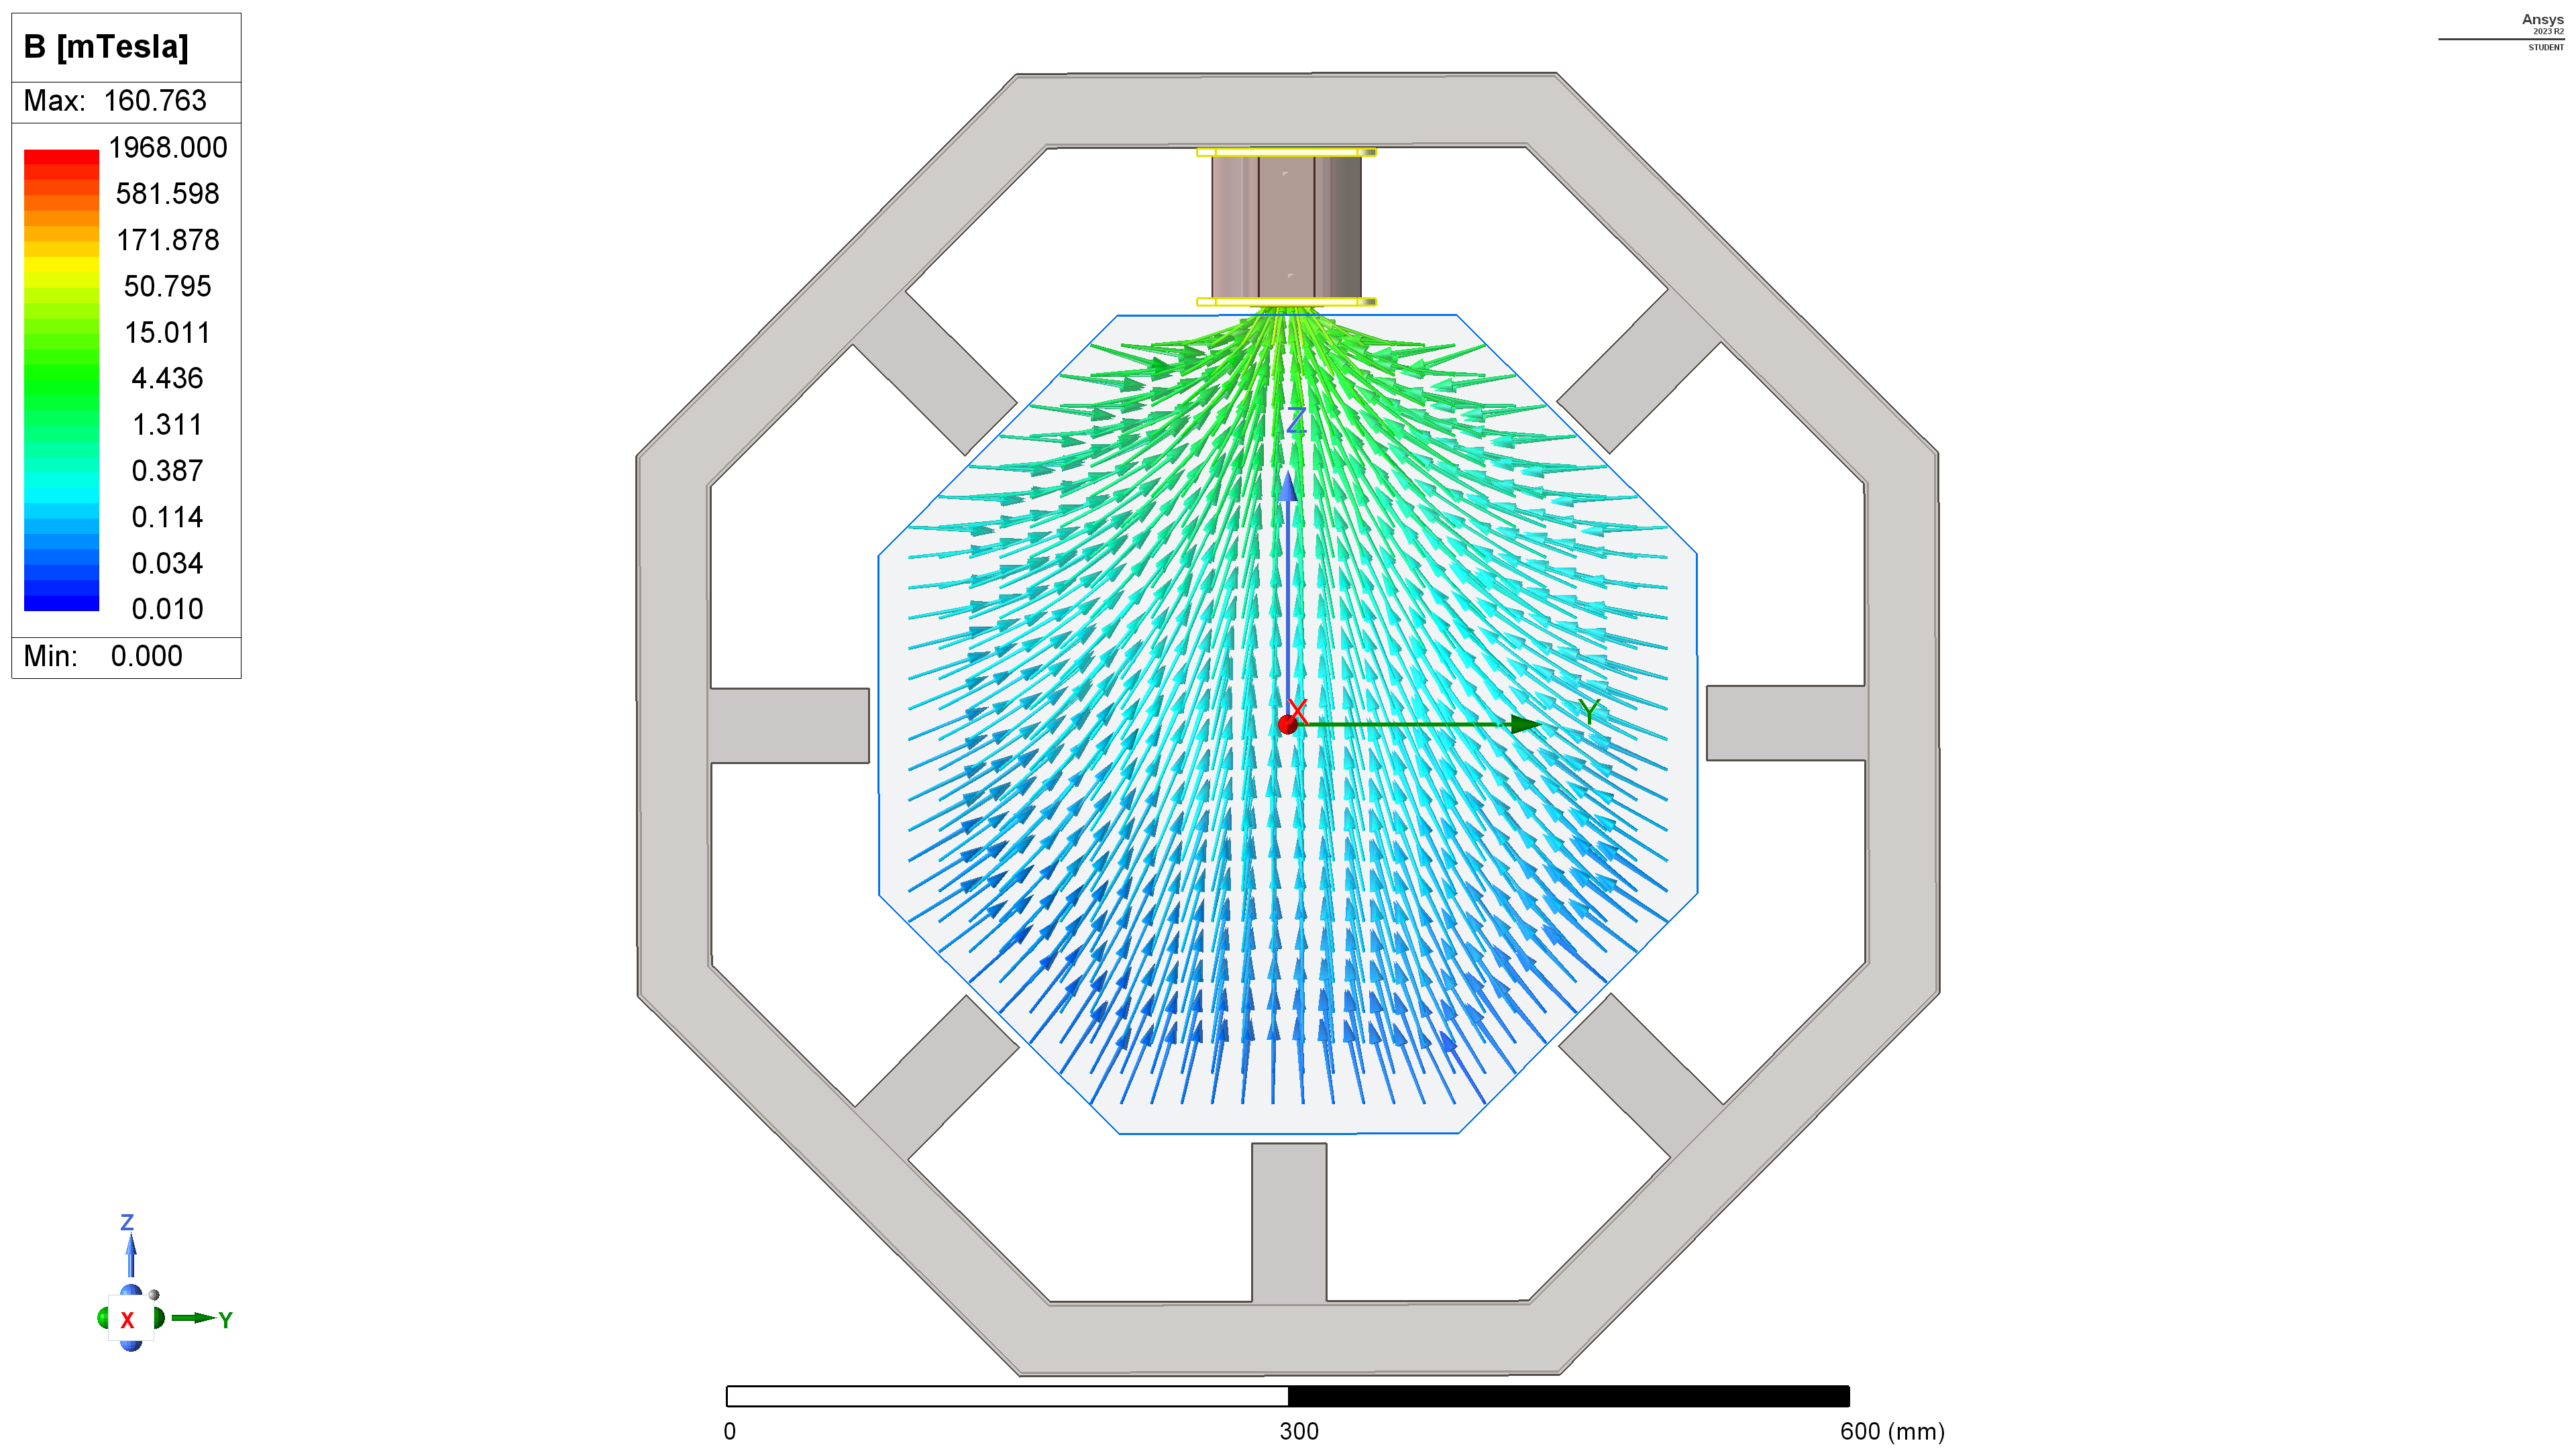
\includegraphics[width=\linewidth]{Images/SupportPlastique+FerDansBobine.png}
        \caption{Visualisation des lignes du champ magnétique d'une bobine avec cœur ferromagnétique.}
    \end{minipage}\hfill
\end{figure}
\noindent
Entre ces 2 images ci-dessus, il s'avère que l'utilisation d'un noyau constitué d'un matériau ferromagnétique augmente significativement l'intensité du champ magnétique et de son gradient. À ce stade, un simple test constitué d'une bobine et d'une barre en acier plein en son centre a été réalisé pour vérifier les résultats de la simulation et a permis de confirmer qu'il est possible d'attirer le microrobot jusqu'à une distance de 45 cm de la bobine. \\Mieux encore, l'ajout d'une structure octogonale ferromagnétique permet de boucler le champ magnétique, et donc de renforcer celui-ci dans l'entrefer.
\begin{figure}[H]
    \centering
    \begin{minipage}{0.45\textwidth}
        \centering
        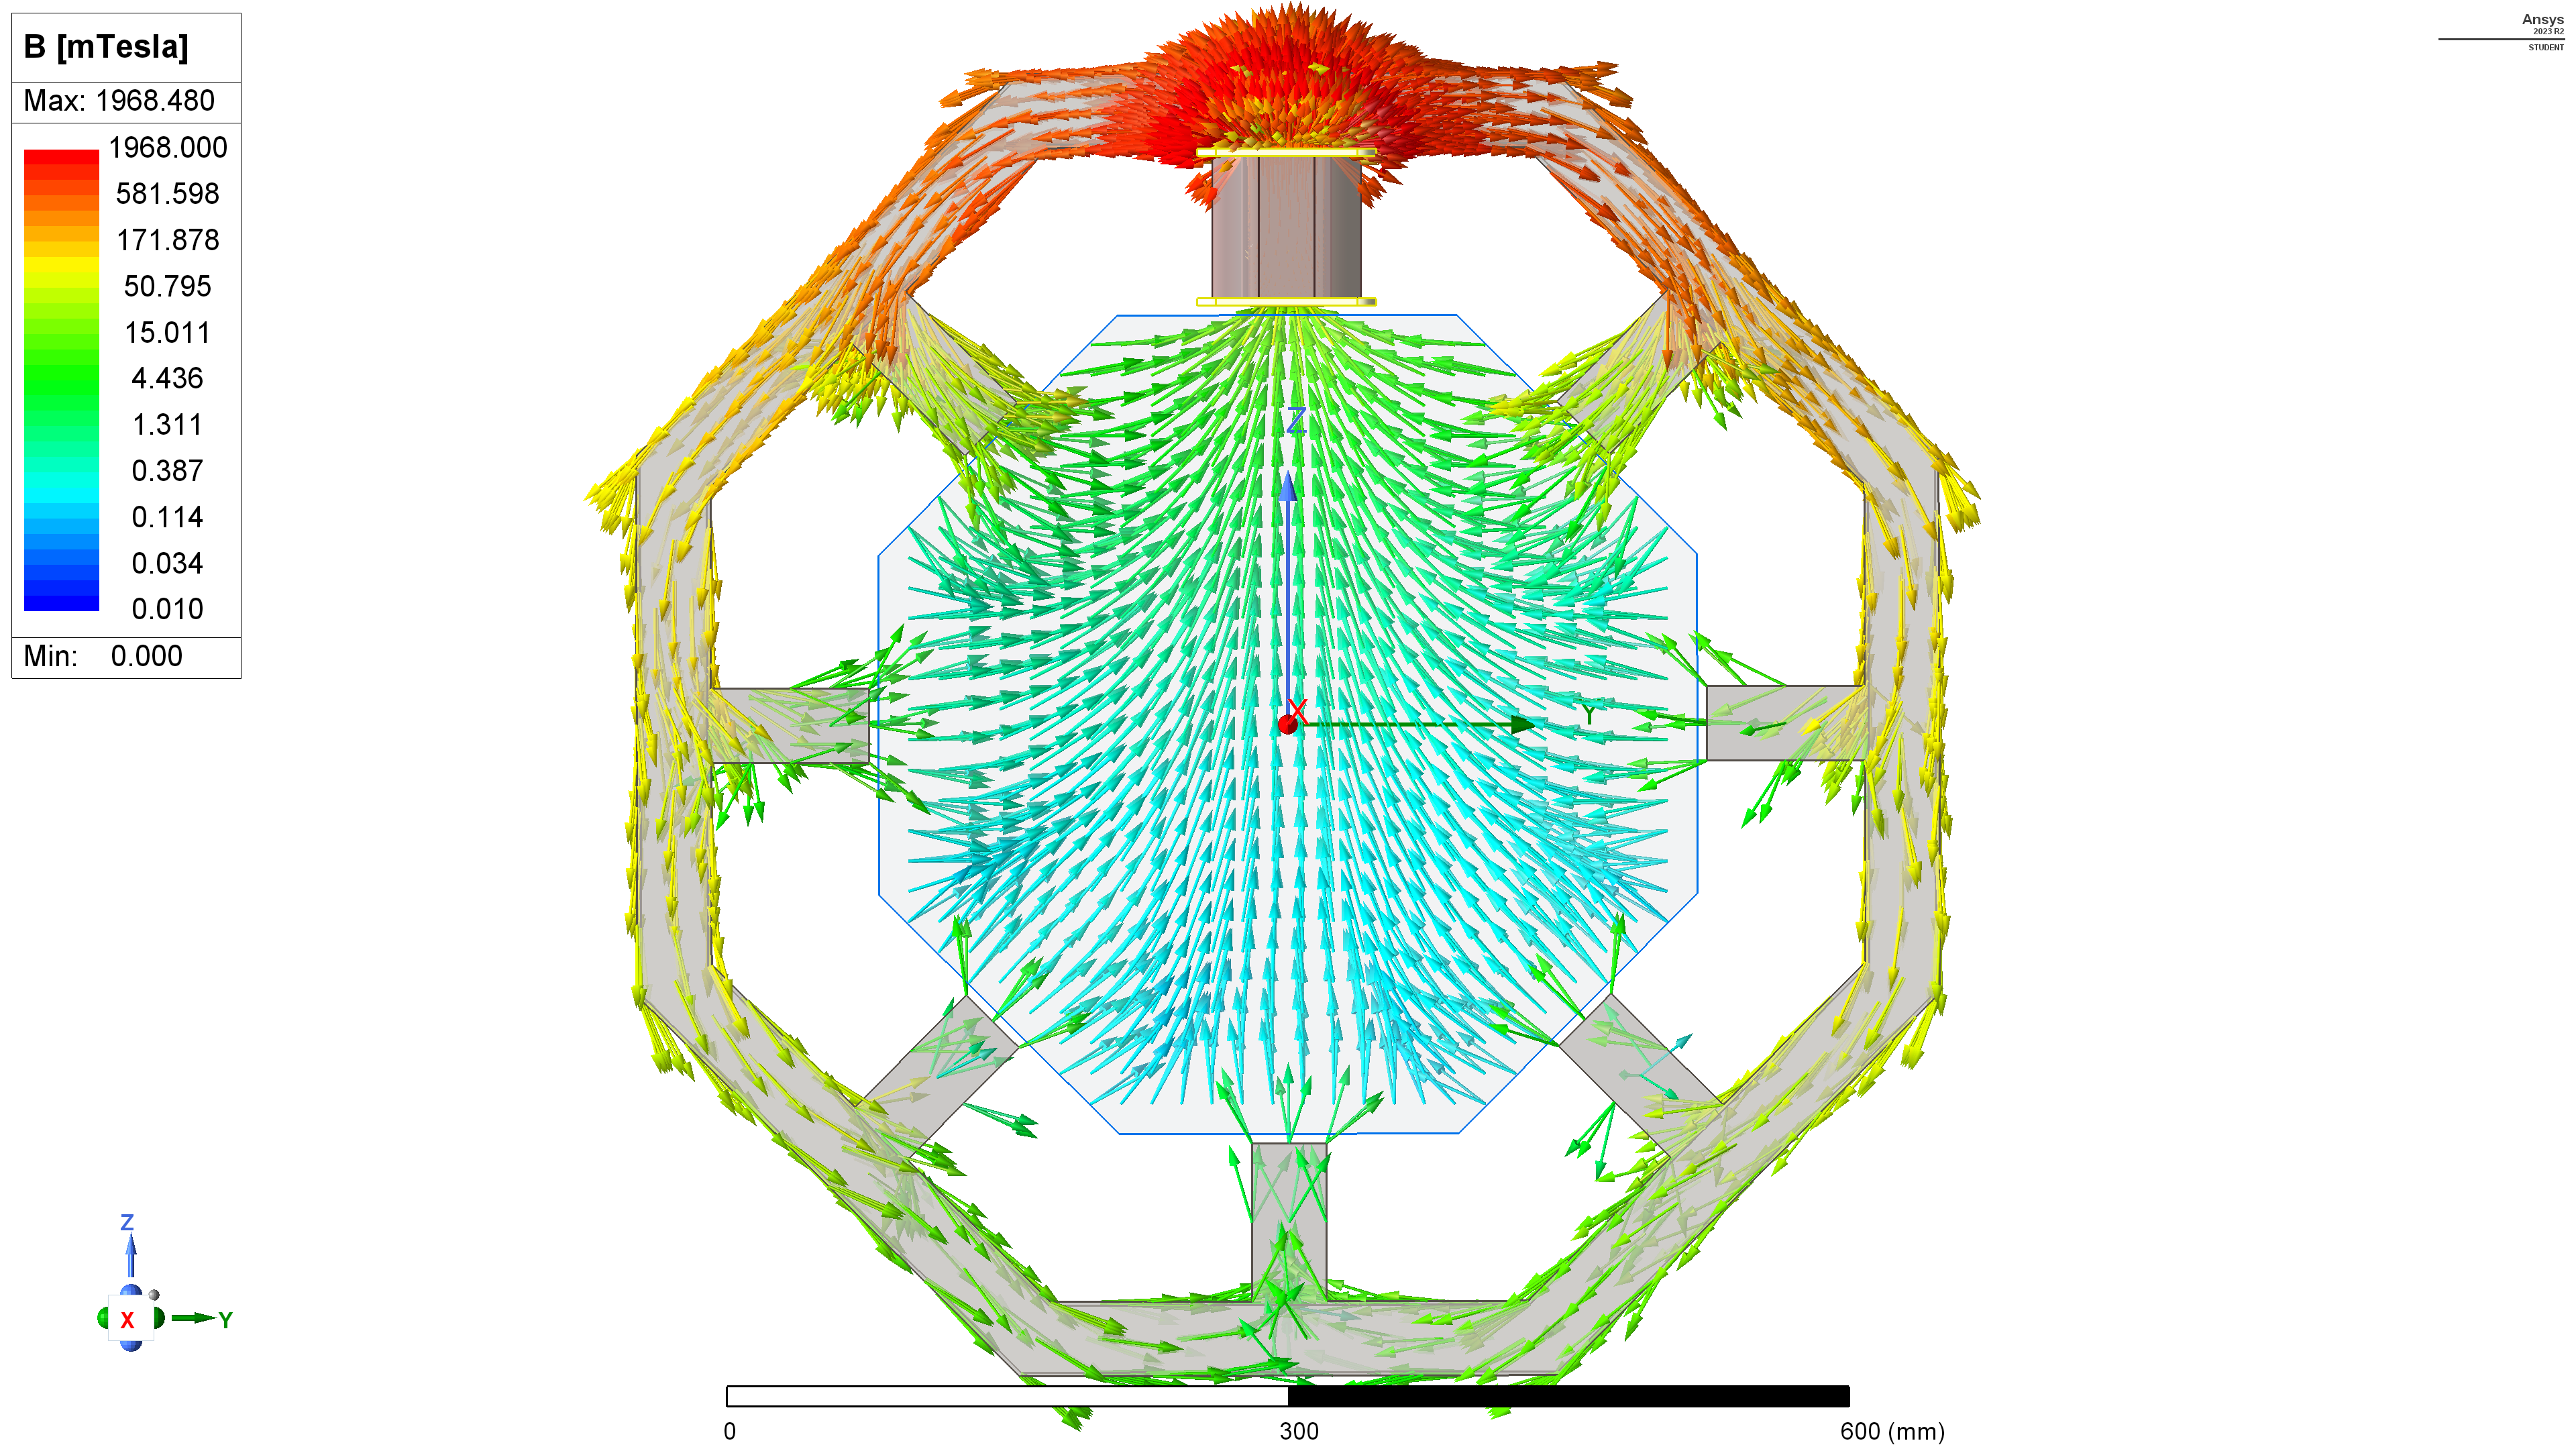
\includegraphics[width=\linewidth]{Images/B1-5,0.png}
        \caption{Visualisation des lignes du champ magnétique d'une bobine avec cœur et structure ferromagnétique.}
    \end{minipage}\hfill
    \begin{minipage}{0.45\textwidth}
        \centering
        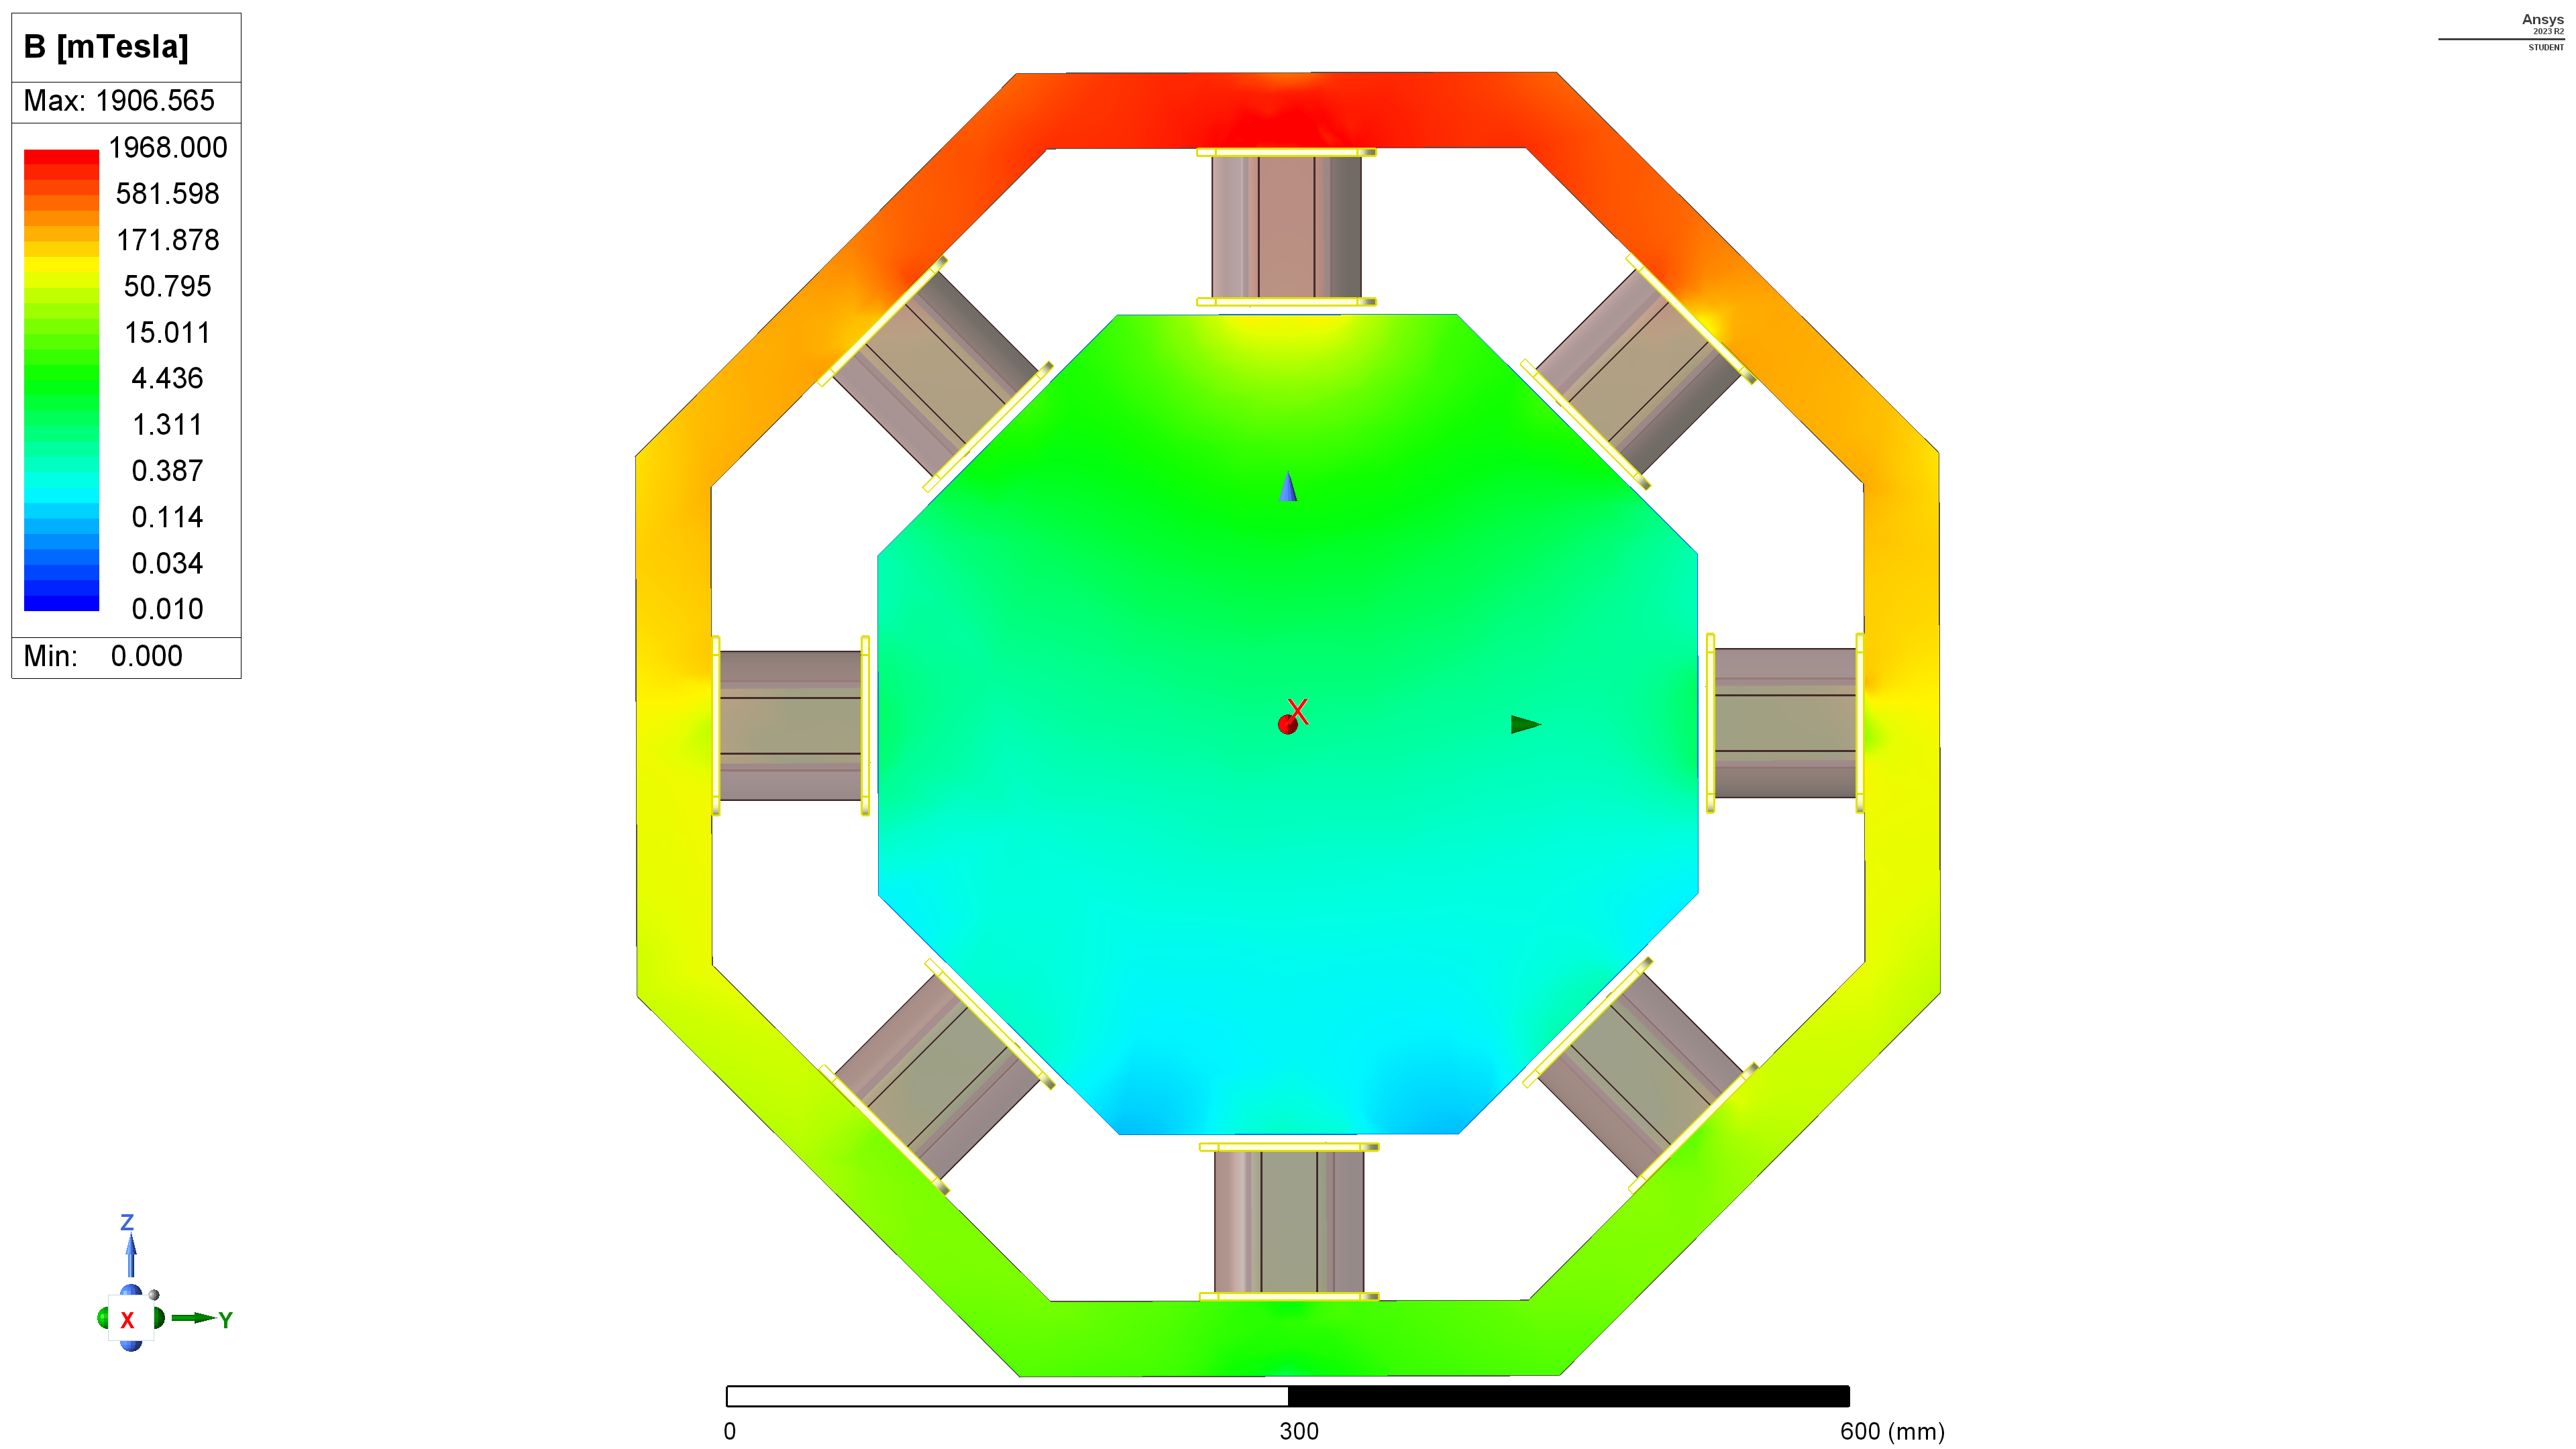
\includegraphics[width=\linewidth]{Images/B1-5,0_Magnitude.png}
        \caption{Visualisation de la magnitude du champ magnétique d'une bobine avec cœur et structure ferromagnétique.}
    \end{minipage}\hfill

\end{figure}
\noindent
D'après les simulations, cette option devrait encore augmenter la force appliquée sur le microrobot. Cependant, faute de pouvoir tester cette configuration sans l'avoir construite, il a été choisi de garder une distance de 45 cm, car cela est suffisant, et le microrobot accélérera donc plus vite.\\\\Cependant, cette configuration pose un petit problème visible sur la figure ci-dessus, puisque le champ magnétique est bouclé et qu'il y a 8 emplacements pour les bobines, cela permet aux lignes de champ de "ressortir" du métal sur les côtés. Pour éviter cela, il est donc nécessaire d'annuler ces retours de champ en allumant les autres bobines dans le sens opposé avec un courant adéquat.
\begin{figure}[H]
    \centering
    \begin{minipage}{0.45\textwidth}
        \centering
        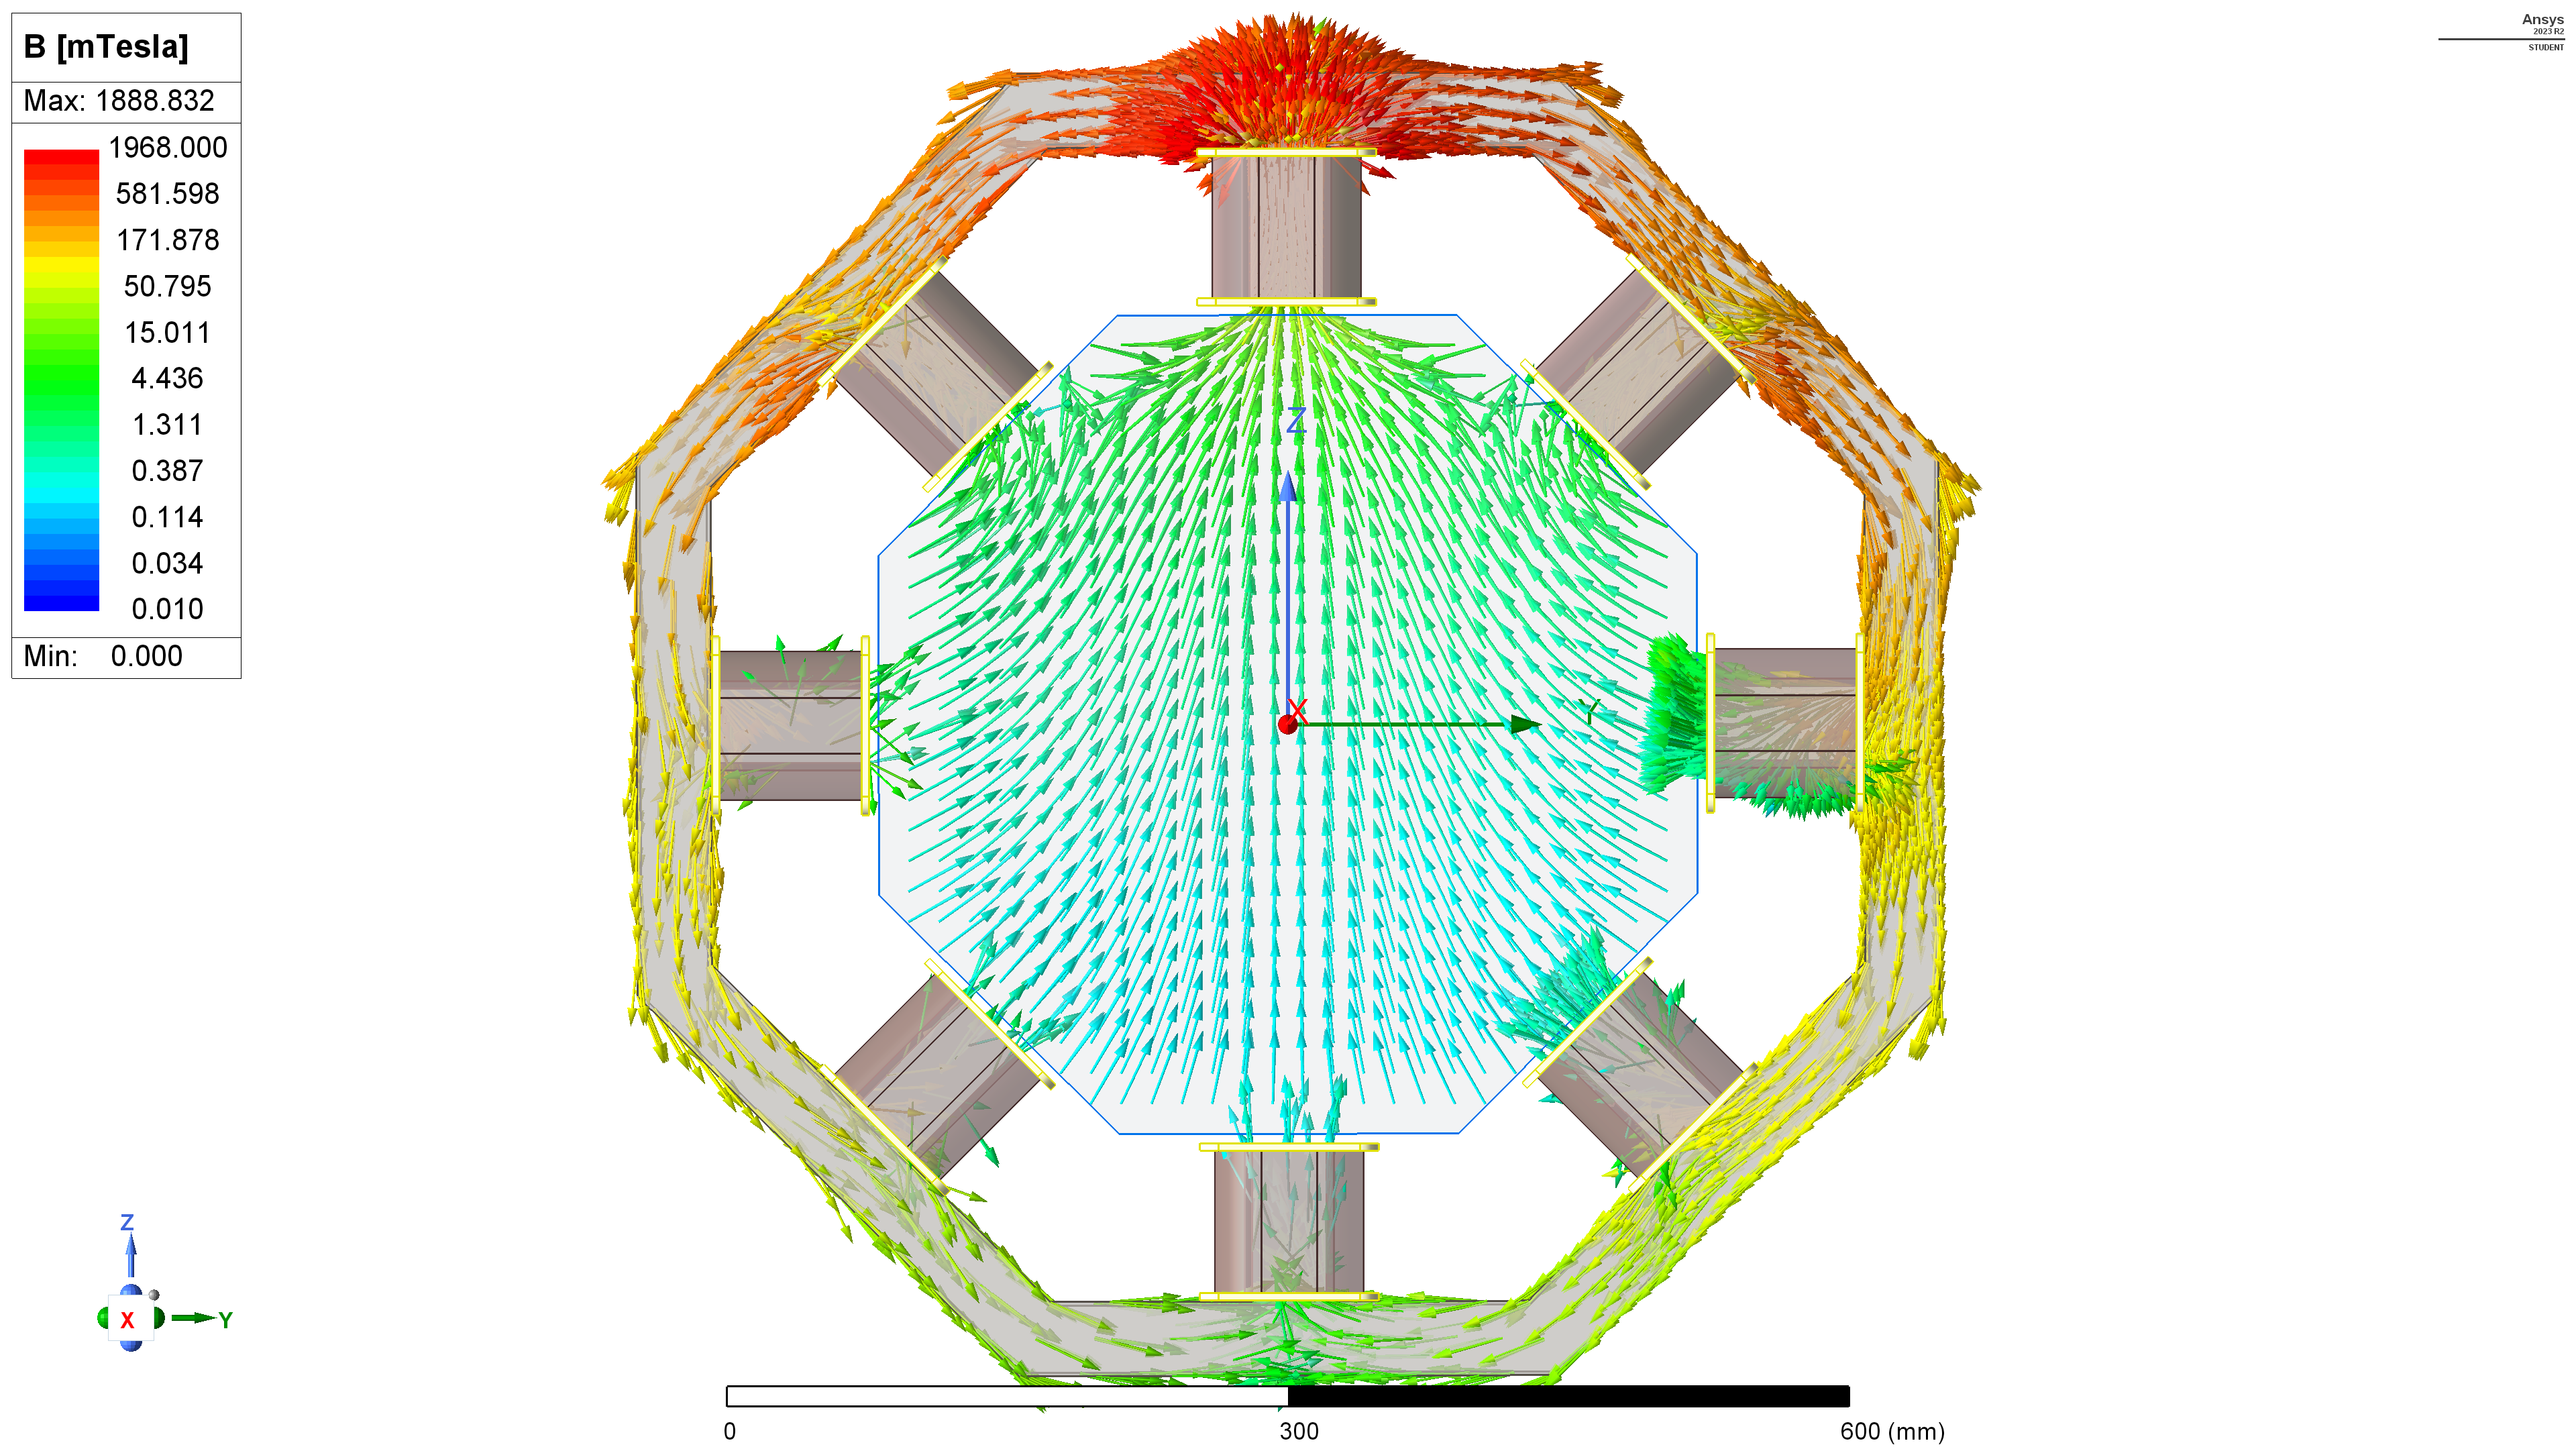
\includegraphics[width=\linewidth]{Images/B1-5_B2-0,8_B3-0,1_B4-0,04_B5-0,03_B6-0,04_B7-0,1_B8-0,8.png}
        \caption{Visualisation des lignes du champ magnétique d'une bobine avec cœur et structure ferromagnétique ainsi que l'atténuation des effets indésirables par les autres bobines.}
    \end{minipage}\hfill
    \begin{minipage}{0.45\textwidth}
        \centering
        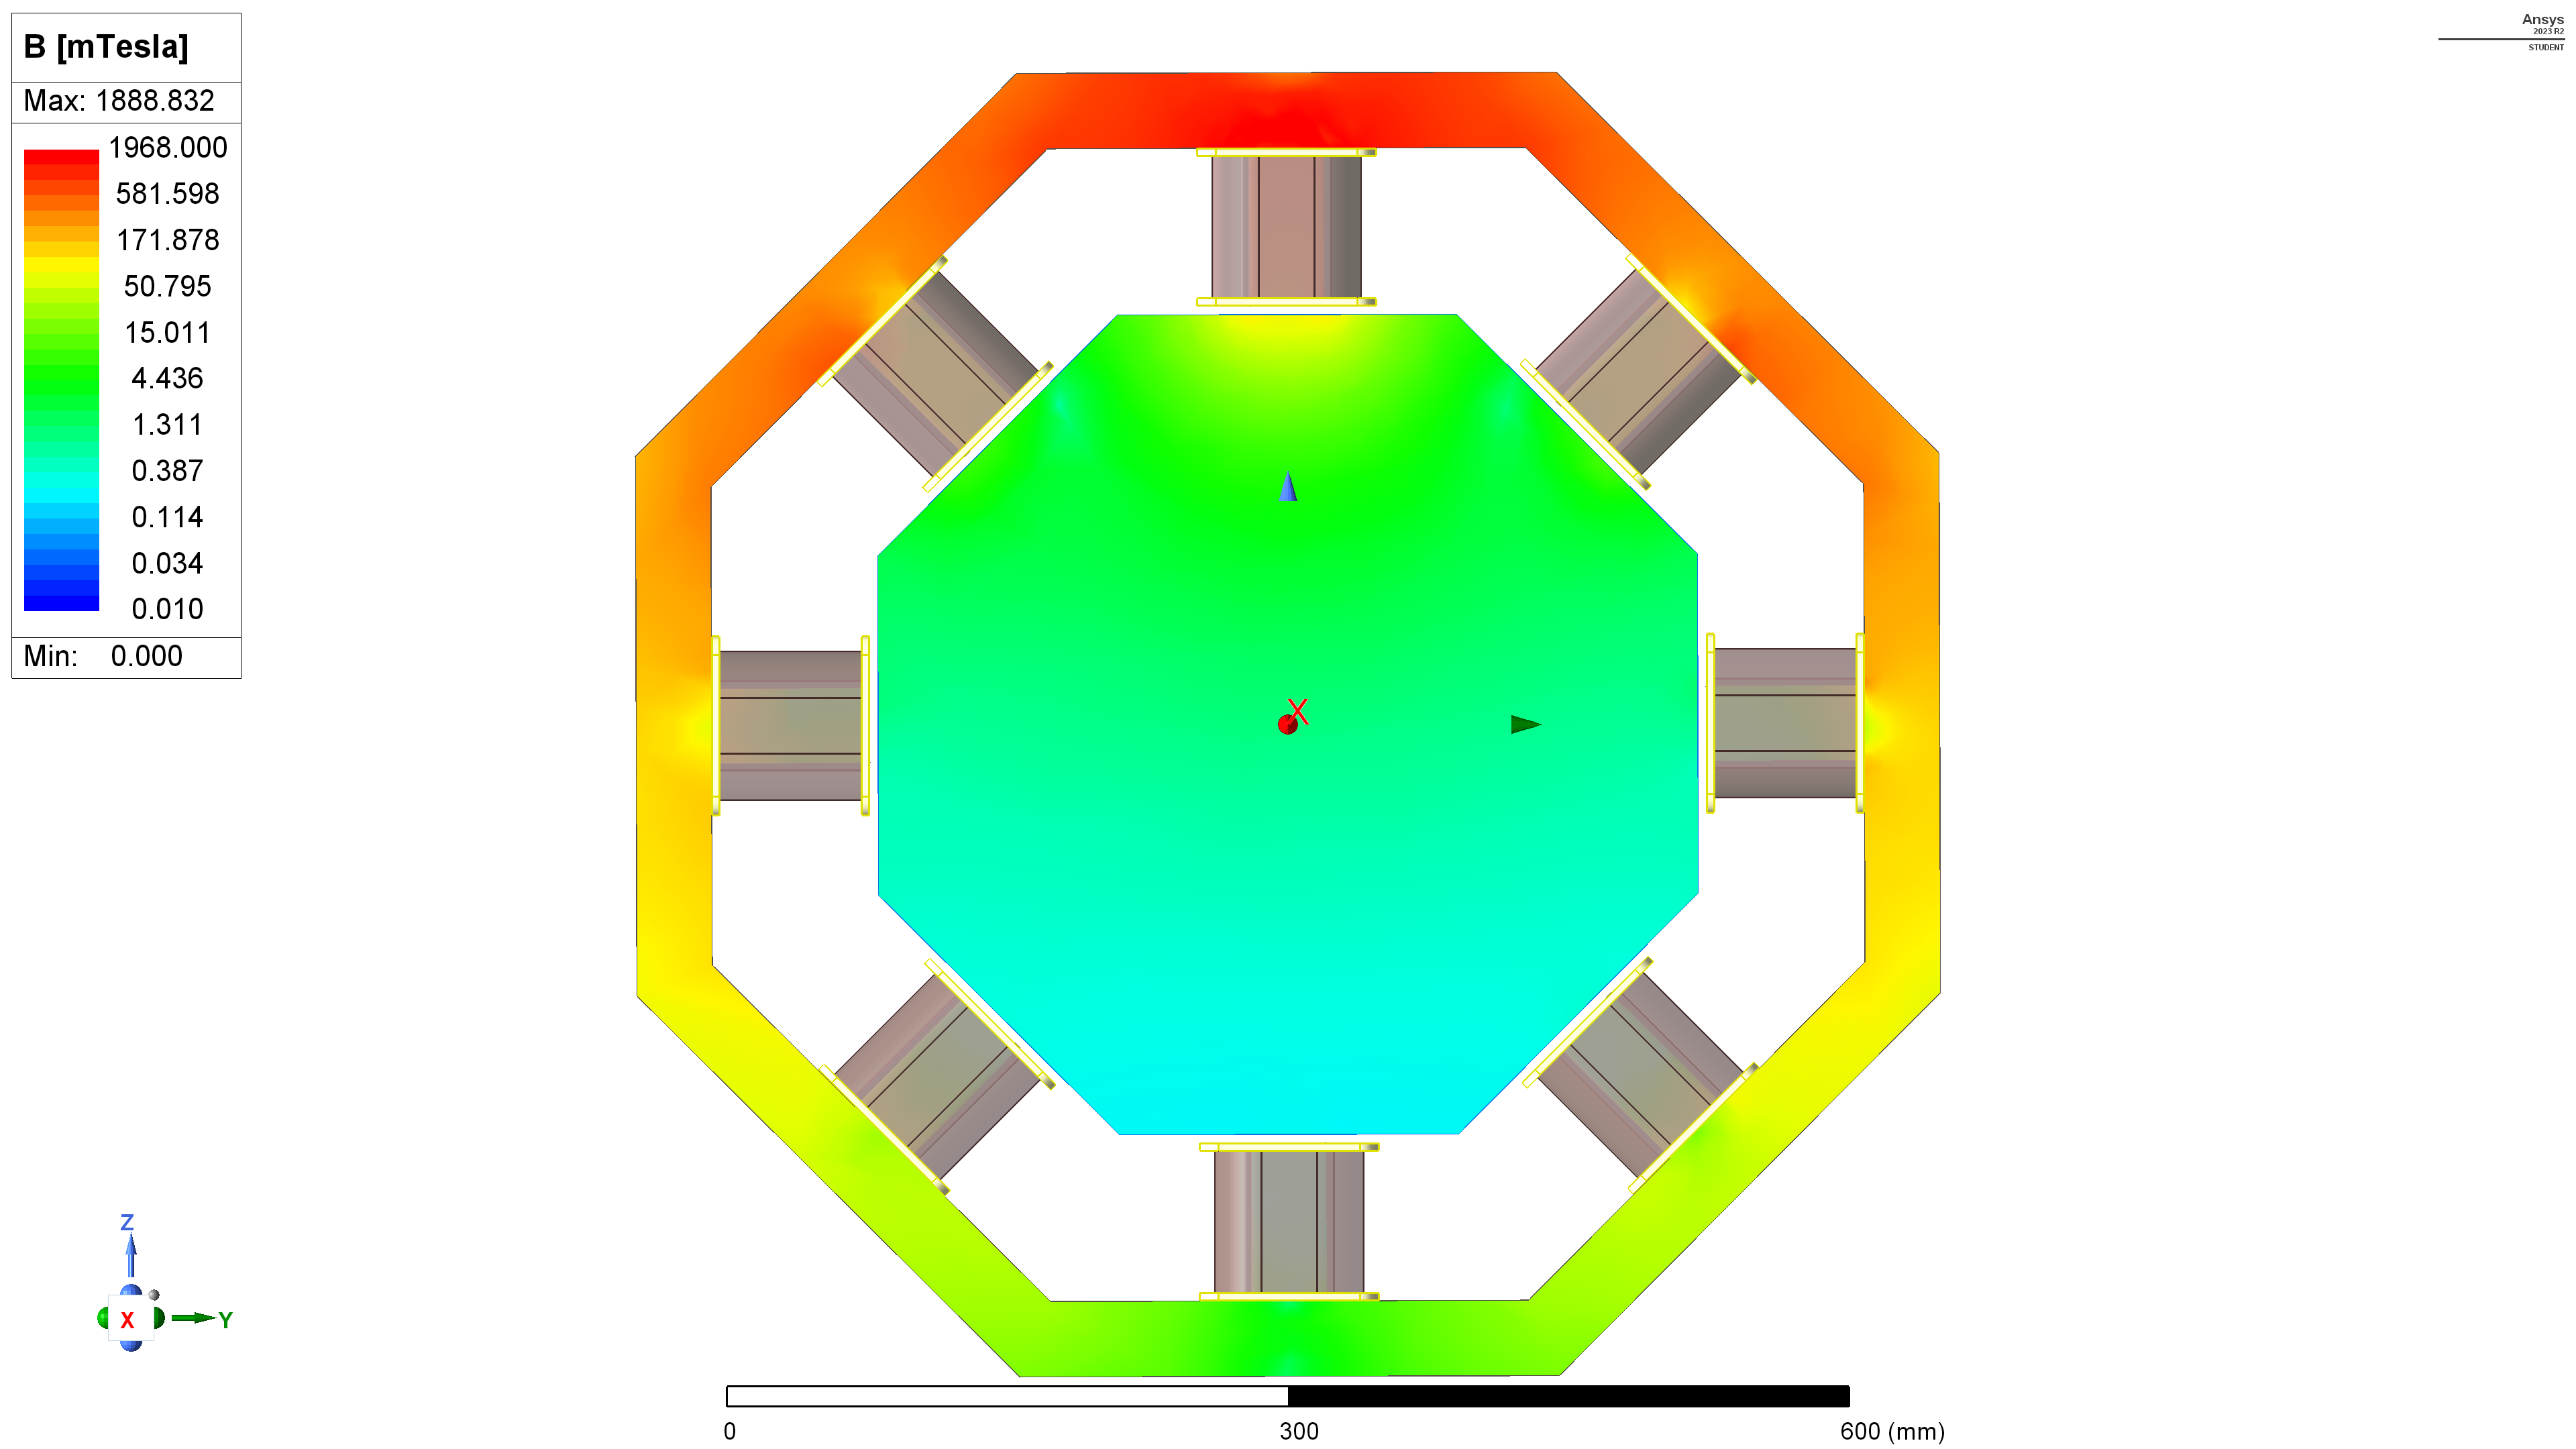
\includegraphics[width=\linewidth]{Images/B1-5_B2-0,8_B3-0,1_B4-0,04_B5-0,03_B6-0,04_B7-0,1_B8-0,8_Magnitude.png}
        \caption{Visualisation de la magnitude du champ magnétique d'une bobine avec cœur et structure ferromagnétique ainsi que l'atténuation des effets indésirables par les autres bobines.}
    \end{minipage}\hfill

\end{figure}
\noindent
Le dernier petit problème est que pour fabriquer cette structure, il aurait fallu un matériau ferromagnétique doux, tel que celui utilisé dans les transformateurs. Au vu du budget et de la forme spécifique du système, un simple acier classique a été utilisé. Cela implique donc qu'à l'arrêt des bobines, il reste une rémanence qui peut attirer le microrobot. Cette rémanence devra aussi être annulée en inversant le courant dans les bobines.

%\newpage
\section{Électronique de puissance pour la gestion des courants dans les bobines}
Puisque le seul paramètre qu'il est possible de faire varier pour modifier le champ magnétique est l'intensité du courant dans les bobines, il faut trouver un moyen de le contrôler électroniquement pour gérer les 8 bobines. 

\subsection{Détermination de l'intensité admissible dans une bobine}

Les bobines à disposition ont une résistance interne de $2.8 \, \Omega$ pour un fil de cuivre de $1\,mm$ de diamètre et $500$ tours, avec une inductance de $18\, mH$. Ce sont des bobines normalement utilisées en travaux pratiques de physique sur les transformateurs et l'induction. Si l'on considère la bobine alimentée en courant continu, la puissance dissipée est uniquement due à sa résistance $P=R\cdot I^2$.
\\
Selon les données de la figure \ref{fig:courbe_force}, l'application d'un courant d'environ 8A dans une bobine est nécessaire pour générer la force requise afin d'attirer le microdrone à une distance de 45 cm. Bien que la spécification de l'étiquette des bobines soit de 4.5A, ces bobines sont conçues pour des utilisations prolongées et disposent de marges de sécurité considérables pour les travaux pratiques. Les 8A doivent être appliqués de manière très brève et intermittente, limitant ainsi la génération de chaleur. De plus, le diamètre du fil de 1mm offre une capacité adéquate pour gérer de tels courants de manière ponctuelle sans risque de dommage.
\\
Les alimentations à tension fixe et courant continu disponibles dans le commerce à un prix raisonnable sont très souvent à des valeurs de tension prédéfinies (5V, 12V, 24V, 48V...). Pour des raisons de sécurité, il est préférable de ne pas travailler avec des tensions trop élevées.\\Pour fournir un courant proche de la valeur limite fixée, une simple application de la loi d'Ohm $U=R\cdot I$ permet de choisir une alimentation de $24 \,V$. L'alimentation trouvée est capable de fournir $50 \,A$, soit $1200 \,W$. \\Puisque à pleine puissance une bobine consomme $P=\frac{U^2}{R}$ soit $\frac{24^2}{2.8} = 206 \,W$.
\\\\
Il est donc nécessaire de faire très attention à ne pas alimenter plus de 5 bobines à la fois à pleine puissance. En pratique, il n'est généralement pas nécessaire d'allumer simultanément plus de 2 ou 3 bobines à leur maximum. Par mesure de sécurité et pour protéger l'alimentation, un fusible de $40\,A$ est placé en aval de celle-ci.


\subsection{Réalisation d'un circuit électronique de puissance}
Les principales contraintes à prendre en compte sont les suivantes :
\begin{itemize}
    \item Le courant doit pouvoir circuler dans les deux sens.
    \item     Le courant doit pouvoir être ajusté très précisément entre 0 et $I_{\text{max}}$.
    \item Le circuit doit être commandable via un microcontrôleur en utilisant peu de broches de commande.
    \item Le circuit doit être capable de délivrer suffisamment de courant en chauffant le moins possible.
    \item Le circuit ne doit pas utiliser de composants trop coûteux, car il en faut 8 et le budget est limité.

\end{itemize}

Pour répondre à la première contrainte, le plus simple est d'utiliser un pont en H.
    \begin{figure}[H]
    \centering
    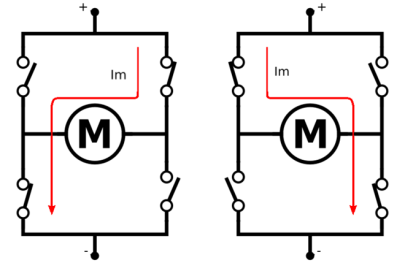
\includegraphics[width=0.25\linewidth]{Images/pontH.png}
    \caption{Schéma de fonctionnement d'un pont en H }
    \label{fig:pontH}
\end{figure}
\noindent
Les interrupteurs de droite constituent un bras de pont, et ceux de gauche un autre. De cette manière, en allumant de manière complémentaire l'un des deux interrupteurs de chaque bras de pont, le courant circule dans l'un ou l'autre sens. Pour rendre ceci contrôlable électroniquement, les interrupteurs sont remplacés par des transistors
\\
\\
Maintenant, pour ajuster la valeur du courant, plusieurs options sont envisageables:

-La première serait d'utiliser un amplificateur intégré de puissance. Bien que simple à utiliser, cela coûte environ une dizaine d'euros par pièce pour un courant de sortie de quelques ampères, et devient beaucoup trop cher pour une dizaine d'ampères et plus.

-Une autre option serait d'utiliser un hacheur et de lisser le courant, à la manière d'un convertisseur abaisseur (buck). Cependant, les charges sont des bobines fixes, ce qui présente l'avantage d'avoir déjà une inductance interne. Il est donc possible d'utiliser un hacheur avec une fréquence adéquate pour que les bobines se chargent de lisser le courant.
De plus, la structure du pont en H contient déjà des transistors permettant d'activer ou non les bobines. Il suffit donc de combiner les caractéristiques d'un hacheur avec celles du pont en H.
\\\\
Des circuits tout faits de ce type sont disponibles dans le commerce, notamment dans le monde du modélisme/drones avec les ESC (Electronic Speed Controllers) pour moteurs à balais. Cependant, ils peuvent être assez coûteux, surtout s'il en faut 8, et ils ont déjà un microcontrôleur interne avec un programme et une fréquence de découpage optimisés pour un petit moteur, ce qui limite le contrôle sur les signaux de sortie dans les bobines.
\\\\
Il a donc été choisi de concevoir un hacheur avec un pont en H.
\\
En principe, il suffit de remplacer tous les interrupteurs du pont en H par des transistors MOSFET et d'envoyer un signal PWM (Pulse Width Modulation) sur l'un des deux transistors passants.

  \begin{figure}[H]
    \centering
    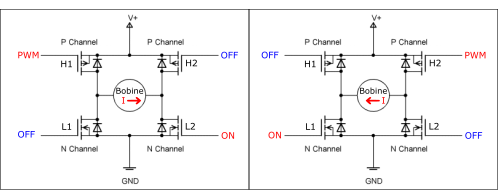
\includegraphics[width=0.7\linewidth]{Images/pontH_Mosfet.png}
    \caption{Schéma de principe du hacheur quatre quadrants}
    \label{fig:pontH_mosfet}
\end{figure}
\noindent
Les transistors H1 et H2 sont des MOSFET canal P, tandis que les L1 et L2 sont des MOSFET canal N .
\\
Pour le canal N, le transistor conduit lorsqu'une tension positive est appliquée sur la broche Gate et il agit comme un interrupteur polarisé sur le 0 V. Pour que le transistor N conduise, la tension de seuil de grille-source (VGS) doit être inférieure à zéro.
\\
En revanche, pour le canal P, le MOSFET est complémentaire au canal N ; le transistor conduit lorsque la tension de commande est inférieure à $V_{+}$. Dans ce cas, la tension de seuil de grille-source (VGS) doit être négative pour que le transistor P conduise.
\\\\
Cependant, il n'est pas possible d'utiliser directement les signaux logiques et PWM en sortie d'un microcontrôleur sur les grilles des MOSFET.
\\\\
La fréquence du signal PWM sera déterminée plus tard, mais elle devra quand même être relativement élevée, ce qui conduit à un problème. Pour que le signal soit le plus propre possible, il faut que les temps de montée du transistor MOSFET soient les plus courts possible. Cependant, les MOSFET ne sont pas parfaits et la capacité de la broche gate n'est pas nulle, ce qui entraîne une latence dans le temps de montée. Ce temps de charge est égal à $t=\frac{Q}{I}$, avec $Q$ la charge de la broche Gate et $I$ le courant.
\\\\
Les MOSFET utilisés sont des IRFZ44N, dont la datasheet est disponible en \cite{ref10}. Ce sont des MOSFET canal N très bon marché avec des caractéristiques intéressantes : une résistance Drain-Source de $R_{ds}=17.5\,m\Omega$, une tension Drain-Source $V_{ds}=55\,V$, un courant $I_{ds}=49\,A$, une tension Gate-Source de seuil $V_{gs(th)}=4\,V$, et $V_{gs(max)}\approx 20\,V$ ainsi qu'une charge totale de Gate $Q_{g}=63\,nC$. Ces caractéristiques sont bien adaptées aux contraintes du circuit, offrant une marge importante sur les courants et tensions admissibles. Pour limiter la chauffe du composant, il faut travailler dans sa zone saturée afin de bénéficier de la valeur minimale de $R_{ds}$. Pour cela, il faut appliquer une tension $V_{gs(th)}<V_{gs}<V_{gs(max)}$. Une tension $V_{gs}$ de $12\,V$ est suffisante. Il faudra donc amplifier la tension des sorties du microcontrôleur vers $12\,V$ pour commuter pleinement le transistor.
\\
Ces deux raisons, ainsi que d'autres, imposent d'utiliser des drivers de Gates pour piloter les MOSFET.
\\\\
Pour les premiers tests, des drivers de type TC4427 \cite{ref11} étaient disponibles à l'ISEN. Faciles d'utilisation, il suffit de les alimenter en $12\,V$ et de câbler les entrées sur le microcontrôleur et les sorties sur les grilles des MOSFET.

    \begin{figure}[H]
    \centering
    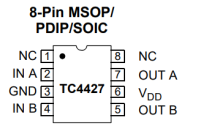
\includegraphics[width=0.25\linewidth]{Images/tc4427.png}
    \caption{Pinout du TC4427
    }
    \label{fig:tc4427}
\end{figure}
\noindent
Cependant, ils ne constituent pas une solution optimale pour le projet final, car le TC4427 accepte une tension maximale de 18V alors que les bobines sont alimentées en 24V. De plus, comme expliqué précédemment, il faut des MOSFET canal P pour les transistors haut (H1/2) et canal N (L1/2). Mais les transistors canal P sont plus complexes à fabriquer et ont donc un coût plus élevé. Le prix reste encore acceptable, mais en revanche, leur résistance $R_{ds}$ est bien plus élevée que pour les canal N, ce qui va générer une dissipation thermique plus importante.
\\\\
Une autre solution, plus complexe mais mieux optimisée, consiste à utiliser uniquement des MOSFET canal N et à les piloter avec une tension de grille supérieure à la tension d'alimentation. Ce montage est appelé un contrôle en "HIGH side".
Pour ce faire il faut utiliser un circuit capable d'augmenter la tension a une valeur superieur de la tension d'alimentation. "Le bootstrap",  est une technique couramment utilisée dans les circuits électroniques pour améliorer l'efficacité et les performances des amplificateurs ou des dispositifs de commutation.\\
Le bootstrap permet de contrôler un MOSFET à partir d'un signal de commande à tension plus basse, tout en permettant d'atteindre des tensions de sortie élevées. Le principe de base repose sur l'utilisation d'un condensateur pour stocker une charge électrique puis de l'ajouter a la tension d'alimentation. 
\\\\
Un driver de demi-pont (half-bridge) High side et Low side est alors utilisé, celui-ci contient toute l'électronique nécessaire au pilotage des grilles des MOSFETs. Le driver utilisé est le IR2110 \cite{ref12}.


    \begin{figure}[H]
    \centering
    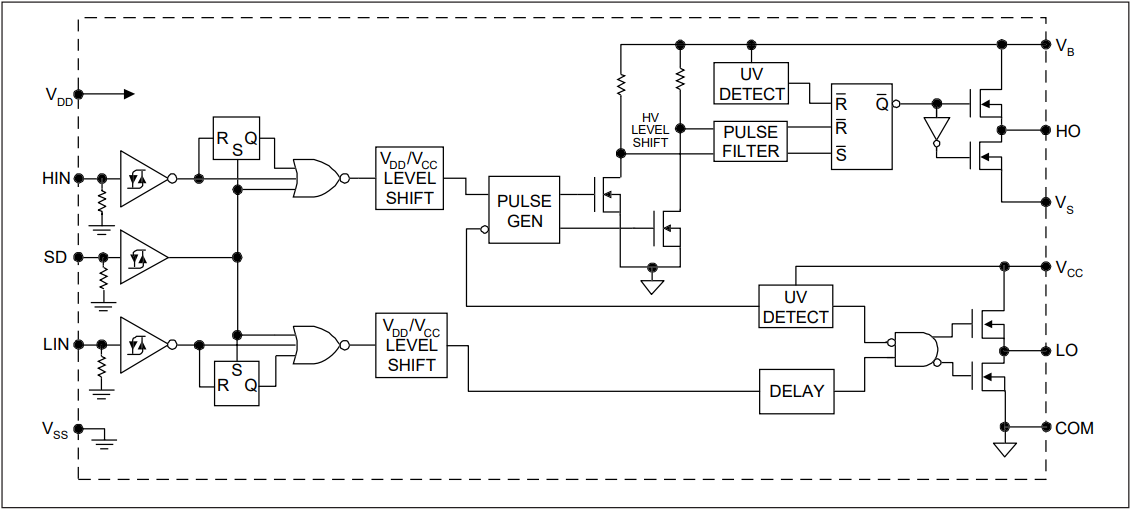
\includegraphics[width=0.5\linewidth]{Images/shema_fonctinel_ir2110.png}
    \caption{Schéma fonctionnel du driver IR2110
    }
    \label{fig:schema_ir2110}
\end{figure}
\noindent
Lorsque le MOSFET L1 est activé, le condensateur se charge à la tension d'alimentation de commutation, ici $12\,V$, comme illustré sur la figure \ref{fig:bootstrap_charge}. Lorsque le MOSFET H1 est activé, le driver utilise ses transistors internes pour positionner le condensateur en série avec la tension d'alimentation des MOSFET, soit $24\,V$ \ref{fig:bootstrap_discharge}. Cela a pour effet d'additionner les deux tensions et permet donc de piloter le MOSFET H1 en mode "High side".

\begin{figure}[H]
    \centering
    \begin{minipage}{0.45\textwidth}
        \centering
        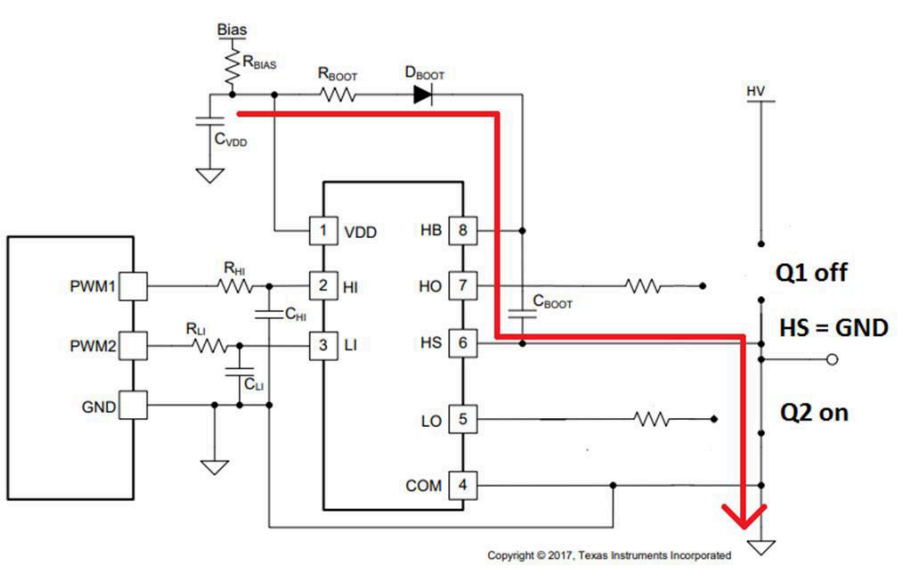
\includegraphics[width=\linewidth]{Images/bootstrap_charge.png}
        \caption{Chemin de charge du condensateur de bootstrap - \cite{ref13}
    }
        \label{fig:fig:bootstrap_charge}
    \end{minipage}\hfill
    \begin{minipage}{0.45\textwidth}
        \centering
        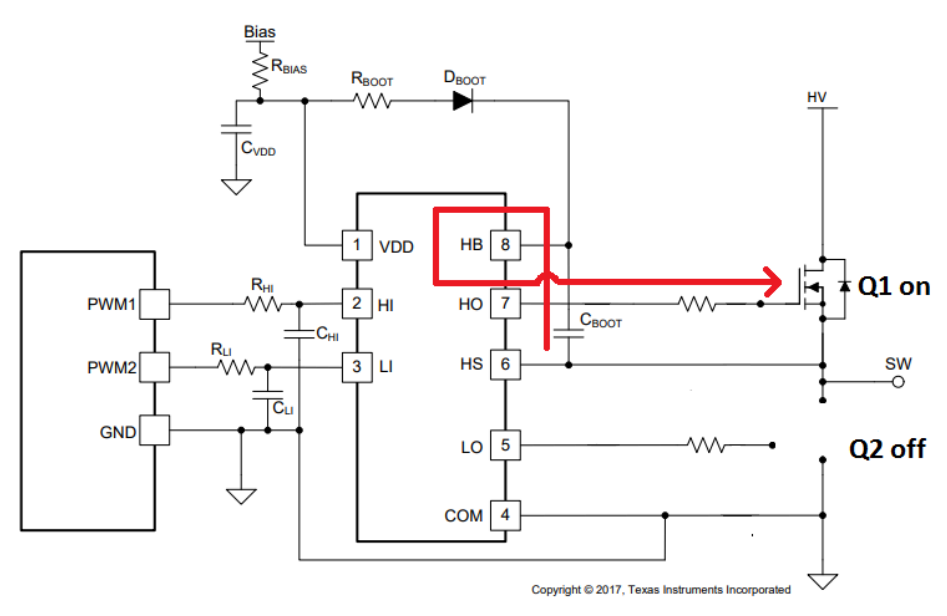
\includegraphics[width=\linewidth]{Images/bootstrap_discharge.png}
        \caption{Chemin de décharge du condensateur de bootstrap - \cite{ref13}}
        \label{fig:bootstrap_discharge}
    \end{minipage}\hfill
\end{figure}
\noindent
D'après le document \cite{ref13}, il faut dimensionner la valeur de manière à ce que $C_{\text{boot}}>10\cdot C_{g}$ avec $C_{g}$ la capacité de grille du MOSFET définie par $C_{g} = \frac{Q_{g}}{V_{dd}-V_{\text{bootDiode}}}$, soit $C_{g} = 2.6\,nF$, donc un $C_{\text{boot}} > 26\,nF$. Pour les tests, seuls des condensateurs de $100\,nF$ étaient disponibles, ce qui est du même ordre de grandeur et respecte la condition sur $C_{\text{boot}}$.

En combinant toutes ces explications, il est possible de réaliser un schéma électronique pour le pilotage d'un bras de pont.
    \begin{figure}[H]
    \centering
    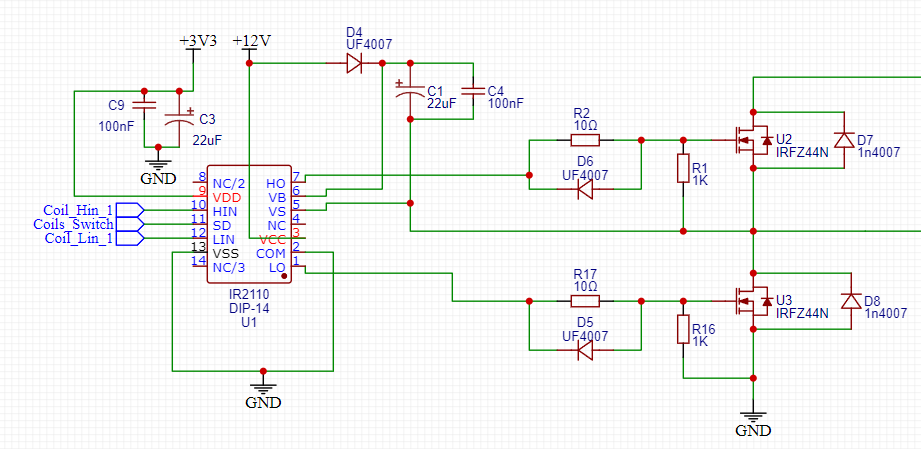
\includegraphics[width=0.7\linewidth]{Images/shemair2110_pontH_demi.png}
    \caption{Schéma de câblage d'un bras de pont (Half bridge)
    }
    \label{fig:half_bridge}
\end{figure}
\noindent
Sur le schéma ci-dessus, il est possible de reconnaître les MOSFET HIGH side et LOW side, les condensateurs et la diode de bootstrap. Cependant, d'autres composants ont été ajoutés :
\begin{itemize}
    \item Les diodes D5 et D6 ainsi que les résistances R2 et R17 servent respectivement à décharger rapidement la capacité de grille pour réduire les temps de commutation, et les résistances servent à limiter le courant dans la grille.
    \item Les résistances R1 et R16 sont simplement des résistances de pull-down pour éviter d'avoir une entrée flottante sur les grilles lorsqu'elles ne sont pas activées.
    \item Les condensateurs C9 et C3 sont de simples condensateurs de découplage afin de limiter d'éventuelles perturbations.
    \item Les diodes D7 et D8 sont des diodes de roue libre qui servent à protéger les MOSFETs des pics de tension causés par la bobine lors de changements brusques de courant.

\end{itemize}

\noindent Pour obtenir un circuit complet pour le pont en H, il suffit de symétriser le schéma de la figure \ref{fig:half_bridge}, ce qui donne ce schéma :
    \begin{figure}[H]
    \centering
    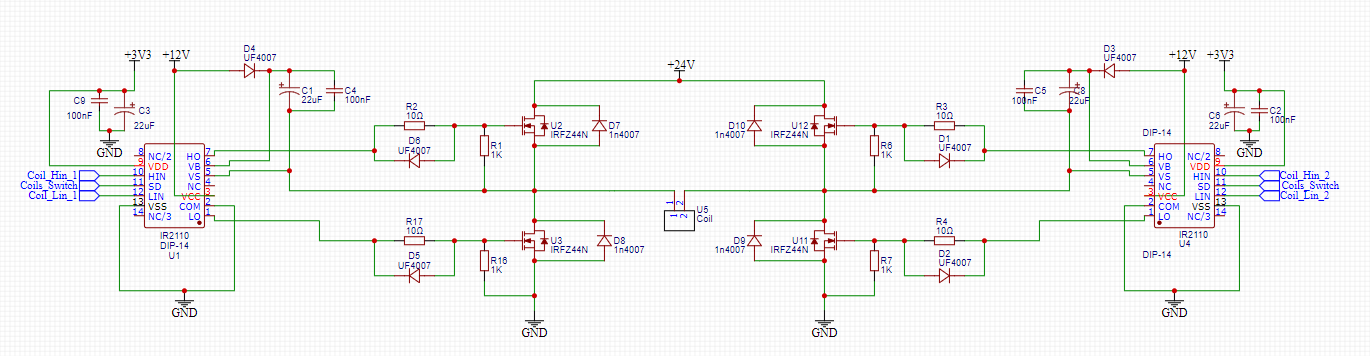
\includegraphics[width=0.7\linewidth]{Images/full_bridge.png}
    \caption{Schéma de câblage du pont en H (Full bridge)
    }
    \label{fig:full_bridge}
\end{figure}
\noindent
Maintenant que ce circuit est fonctionnel, il reste néanmoins un petit problème : il comporte 5 entrées différentes :
\begin{itemize}
    \item Coil\textunderscore Hin\textunderscore 1 (entrée PWM pour le MOSFET H1)
    \item Coil\textunderscore Lin\textunderscore 1 (entrée logique pour le MOSFET L1)
    \item Coil\textunderscore Hin\textunderscore 2 (entrée PWM pour le MOSFET H2)
    \item Coil\textunderscore Lin\textunderscore 2 (entrée logique pour le MOSFET L2)
    \item Coil\textunderscore Switch (active ou désactive les IR2110, un 0 logique = ON)
\end{itemize}

\noindent Cela nécessite au moins 4 broches du microcontrôleur pour piloter les MOSFET et 1 pour activer ou désactiver les drivers. Or, il nous faut 8 cartes, soit 32 broches de commande dont 16 PWM, ce qui n'est pas forcément disponible dans de simples microcontrôleurs. De plus, cela pose un sérieux problème pour l'intégrité des cartes de puissance, car si par erreur le programme du microcontrôleur active simultanément 2 transistors du même bras de pont, cela va tout simplement créer un court-circuit et détruire les transistors.
\\\\
Une solution très simple consiste à observer la logique de commande du circuit. Soit Hin\textunderscore 1 = PWM, Lin\textunderscore 2 = 1 et Hin\textunderscore 2 = 0, Lin\textunderscore 1 = 0, soit l'inverse. Ce qui peut facilement s'écrire dans une table de vérité :
\begin{center}
    \begin{tabular}{|c|c|c|c|c|}
        \hline
        E & Hin\textunderscore 1 & Lin\textunderscore 1 & Hin\textunderscore 2 & Lin\textunderscore 2 \\
        \hline
        0 & PWM & 0 & 0 & 1 \\
        
        1 & 0 & 1 & PWM & 0 \\
        \hline \hline
    \end{tabular}
\end{center}
Il suffit ensuite d'en déduire les équations logiques :
\begin{itemize}
    \item $H_{in1} = \overline{E} \text{ et } \text{PWM}$
    \item $L_{in1} = E$
    \item $H_{in2} = E \text{ et } \text{PWM}$
    \item $L_{in2} = \overline{E}$
\end{itemize}
Afin d'avoir uniquement 2 entrées pour un circuit de puissance, il faut donc  ajouter 2 portes ET et une porte NON dans le circuit. Cela peut être réalisé avec des transistors bipolaires NPN.
\begin{itemize}
    \item Direction (0 ou 1, spécifie le sens dans lequel le pont en H est allumé)
    \item PWM (0\% à 100\%, spécifie la valeur du courant à envoyer dans la bobine)
\end{itemize}

    \begin{figure}[H]
    \centering
    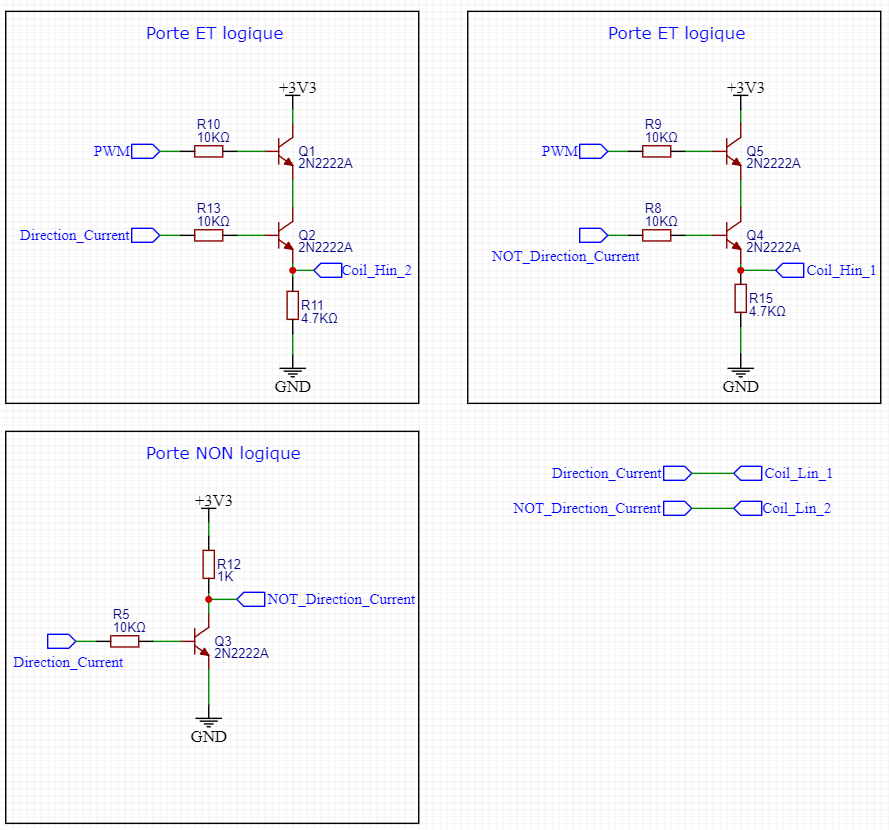
\includegraphics[width=0.45\linewidth]{Images/portes_logiques.png}
    \caption{Schéma de câblage de la logique permettant de réduire le nombre d'entrées
    }
    \label{fig:reduced_input_logic_circuit}
\end{figure}
\noindent
La dernière étape consiste à déterminer la fréquence \( f \) du PWM optimal pour que la bobine suffise à lisser le courant, et donc limiter les fluctuations de courant. Cela peut être calculé en utilisant la formule :

\[ f = \frac{V_{\text{in}} \cdot \alpha(1-\alpha)}{\Delta I \cdot L} \]
Où \( \Delta I \) est l'ondulation de courant, \( V_{\text{in}} \) est la tension d'entrée (\(24\,V\)), \( \alpha \) est le rapport cyclique du PWM et \( L \) est l'inductance de la bobine.
\\
L'ondulation du courant est maximum pour \( \alpha = \frac{1}{2} \), donc pour avoir un \( \Delta I \) faible, de l'ordre de \(10\,mA\), sachant que les bobines ont une inductance de \(18\,mH\), il faut une fréquence de l'ordre de \(10\,kHz\).
\\\\
Voici le prototype sur une breadboard du schéma électronique précédent.:

    \begin{figure}[H]
    \centering
    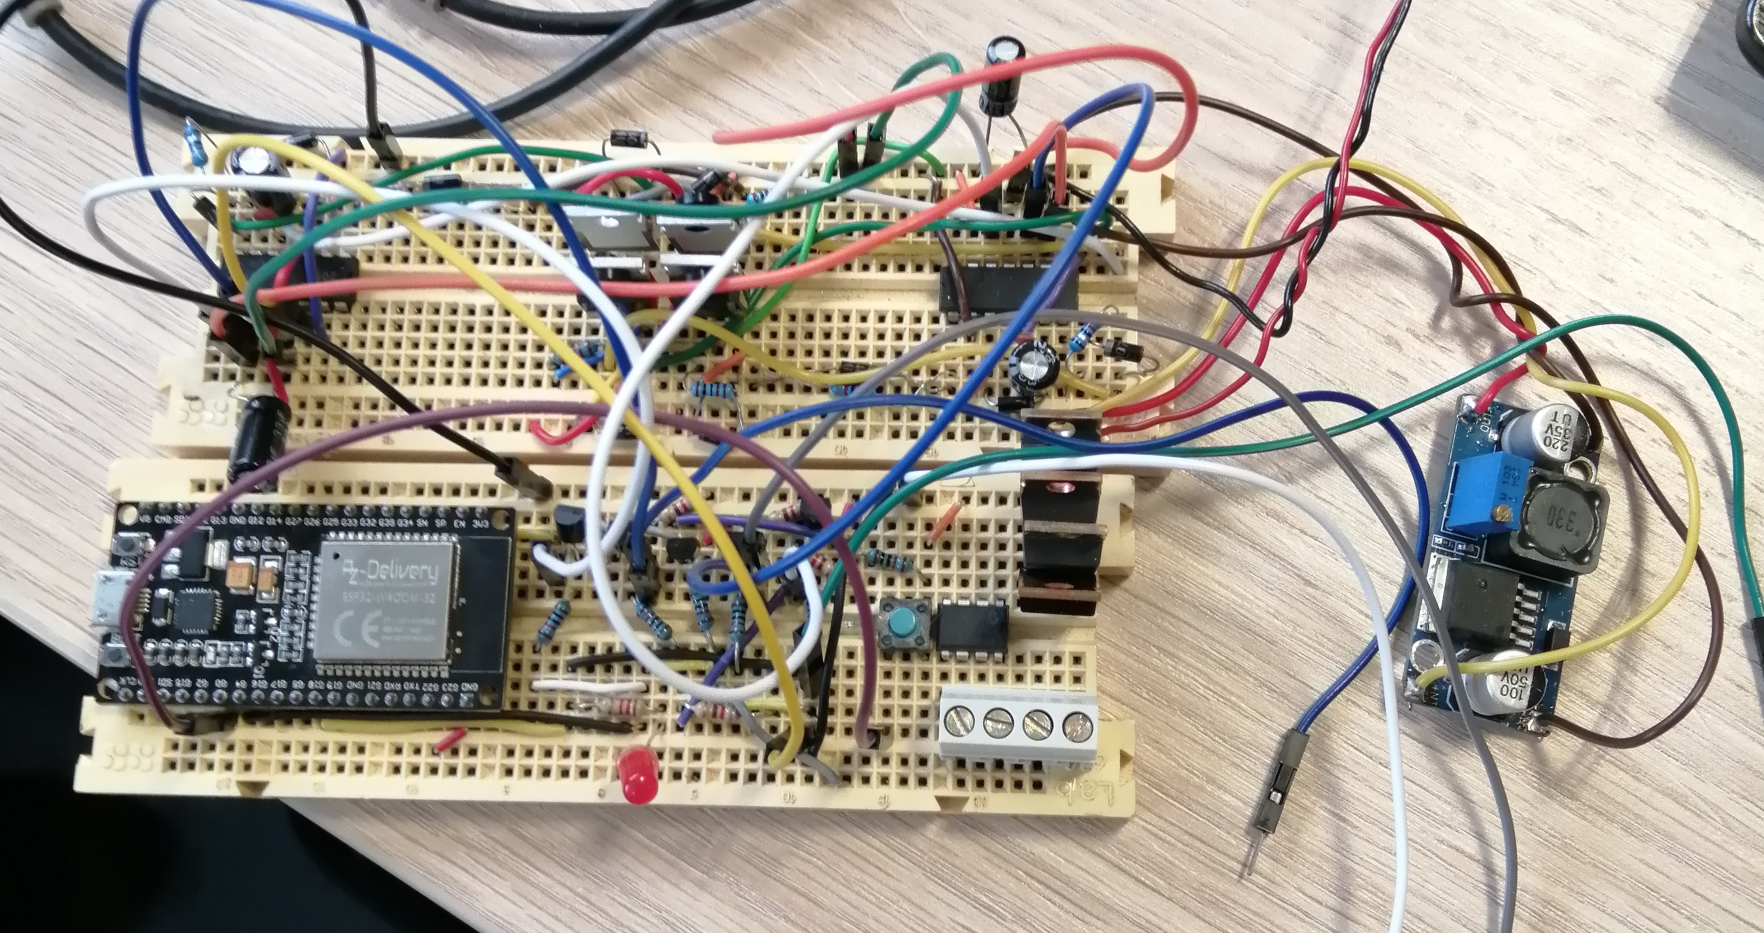
\includegraphics[width=0.5\linewidth]{Images/breadboard.png}
    \caption{Photo du circuit de test assemblé sur 2 breadboards.}
    \label{fig:proto_circuit}
\end{figure}
\noindent
Il est clair qu'il n'est pas envisageable d'utiliser 8 montages de ce type, faits à la main sur des breadboards. Il y a des fils en vrac partout, et la moindre manipulation génère un faux contact. Il est donc nécessaire de créer des circuits imprimés (PCB) sur mesure.

 \subsection{Conception et assemblage des PCB}
Le fabricant de PCB utilisé est JLCPCB, une entreprise spécialisée dans la fabrication de PCB sur mesure, accessible aux particuliers à un prix très abordable. Ils sont reliés à un logiciel de conception nommé EasyEDA, qui contient des fonctionnalités relativement basiques mais qui a l'avantage d'être extrêmement simple à utiliser, surtout au moment de la commande chez JLCPCB. Étant donné la faible complexité des circuits conçus, cela est largement suffisant.
\\\\
Les schémas électroniques utilisés sont exactement les mêmes que ceux de la figure \ref{fig:full_bridge} et \ref{fig:reduced_input_logic_circuit}. Deux LED et quelques connecteurs ont été ajoutés pour visualiser le sens du courant dans la bobine et pour y connecter les différents câbles.
\\\\
Les dimensions du PCB doivent être inférieures à 100mm par 100mm afin de payer moins cher. Initialement, notre professeur encadrant n'était pas très motivé pour que nous fabriquions des PCB. La possibilité de construire 8 cartes à la main sur des plaquettes de prototypage à souder a été envisagée. Les plaquettes disponibles ont une dimension de 50mm par 70mm. Dans l'éventualité où il aurait fallu construire les cartes sur ces plaquettes, un premier placement des composants sur le logiciel permettait d'optimiser un peu les nœuds de connexion pour anticiper la réalisation. C'est pourquoi les dimensions choisies pour les PCB sont d'environ 50mm par 70mm, bien que le routage aurait été plus simple sur une plaque plus grande. \\
Plus tard, notre professeur encadrant a finalement accepté de commander de vrais PCB. Il était donc nécessaire de réaliser un routage complet. Le routage a été réalisé à la main car l'autorouteur disponible ne fonctionne pas très bien. \\\\
Tous les composants sont traversants, car pour des raisons de délais il n'était pas possible de commander des composants de surface. Puisque tout le PCB a été conçu en se basant sur des dimensions relativement petites pour autant de composants traversants, il n'y avait plus de place pour faire des trous pour des vis afin de le fixer. Les dimensions étant inférieures à 100mm par 100mm, il était possible d'ajouter des accroches dans les 4 angles.


     \begin{figure}[H]
    \centering
        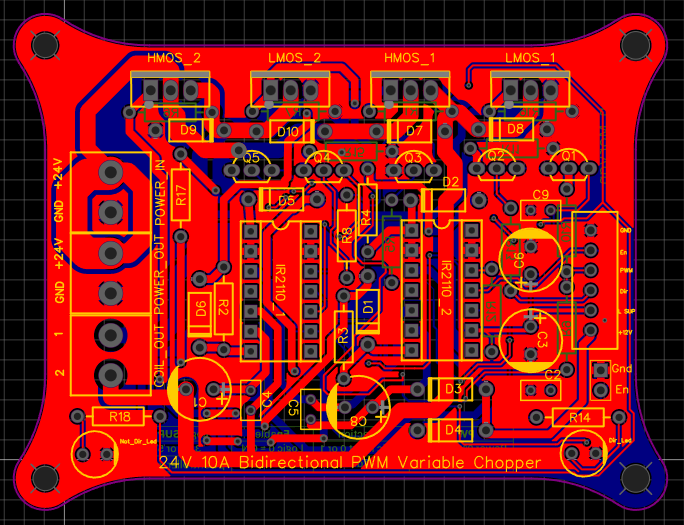
\includegraphics[width = 0.55\textwidth]{Images/PCB_top.png}
        \caption{Vue du dessus du routage du PCB}
        \label{fig:PCB_Top}
    \end{figure}
\noindent
La principale contrainte pour le routage était de pouvoir faire passer suffisamment de courant dans les pistes de puissance. En utilisant un calculateur en ligne de chez DigiKey \cite{ref14}, pour un courant de 8A avec une température ambiante de 20°C, une longueur de piste de quelques centimètres, une augmentation de température acceptable de 15°C et une épaisseur de cuivre de 1oz, il faut une largeur de piste de 4mm.\\Cependant, l'espacement entre les broches des composants est inférieur à 4mm. Les seuls moyens d'avoir des pistes plus fines sont soit, de doubler les pistes sur les deux couches, soit d'utiliser du cuivre plus épais, (2oz), ce qui permet d'avoir des pistes de 2mm. Mais cela ajoute quelques euros sur la carte.
\\\\
Afin de simplifier le câblage des cartes, deux connecteurs d'alimentation sont présents par carte, permettant de brancher les cartes les unes sur les autres. Pour cela, une piste de 4mm et une de 2.5mm sont reliées pour permettre de passer 24A. Il est donc possible de brancher 3 cartes à la suite sans devoir retirer de câble depuis l'alimentation principale.
\\\\
Les MOSFET sont positionnés en bord de carte afin de pouvoir leur installer de petits dissipateurs thermiques, qui malheureusement, au moment de l'écriture de ce rapport, ne sont pas arrivés car le colis s'est perdu.
\\\\
Beaucoup de temps a été perdu sur ces PCB car bien qu'ils étaient prêts à être commandés le 20 mars, cela n'a été fait que la semaine suivante. Et malheureusement, le colis des dissipateurs qui est perdu contenait aussi les drivers de MOSFET, la moitié des MOSFET, les diodes et les connecteurs bananes. Ainsi, jusqu'au 9 avril, il n'était toujours pas possible d'assembler tous les PCB.

\begin{figure}[H]
    \centering
    \begin{minipage}{0.45\textwidth}
        \centering
        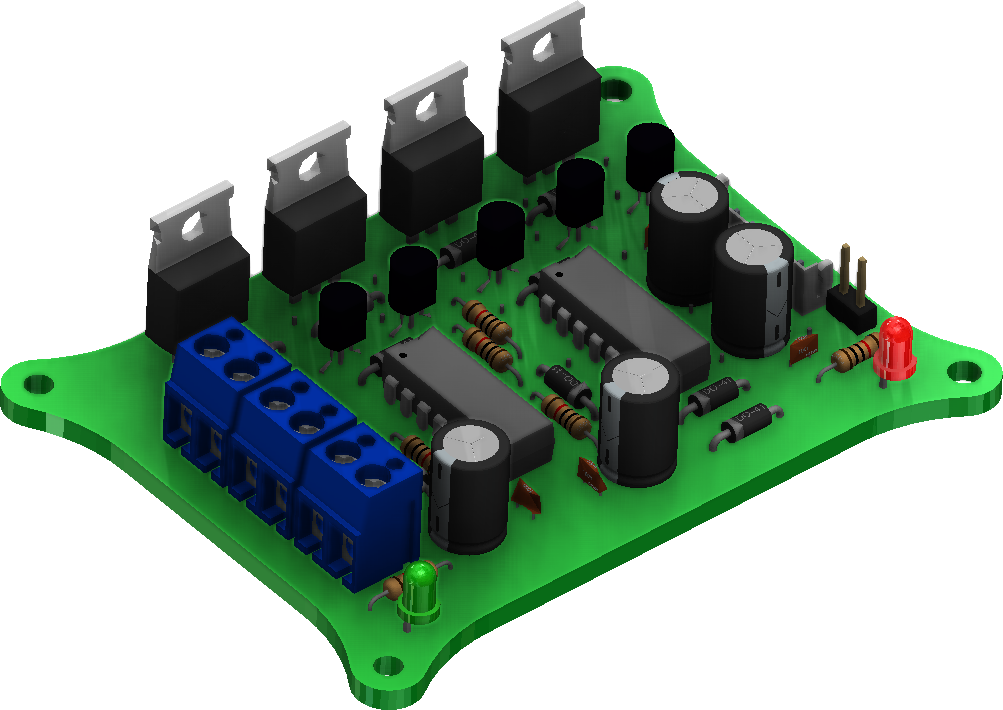
\includegraphics[width=\linewidth]{Images/pcb_3d.png}
        \caption{Vue 3D du PCB}
        \label{fig:PCB_3d-1}
    \end{minipage}\hfill
    \begin{minipage}{0.45\textwidth}
        \centering
        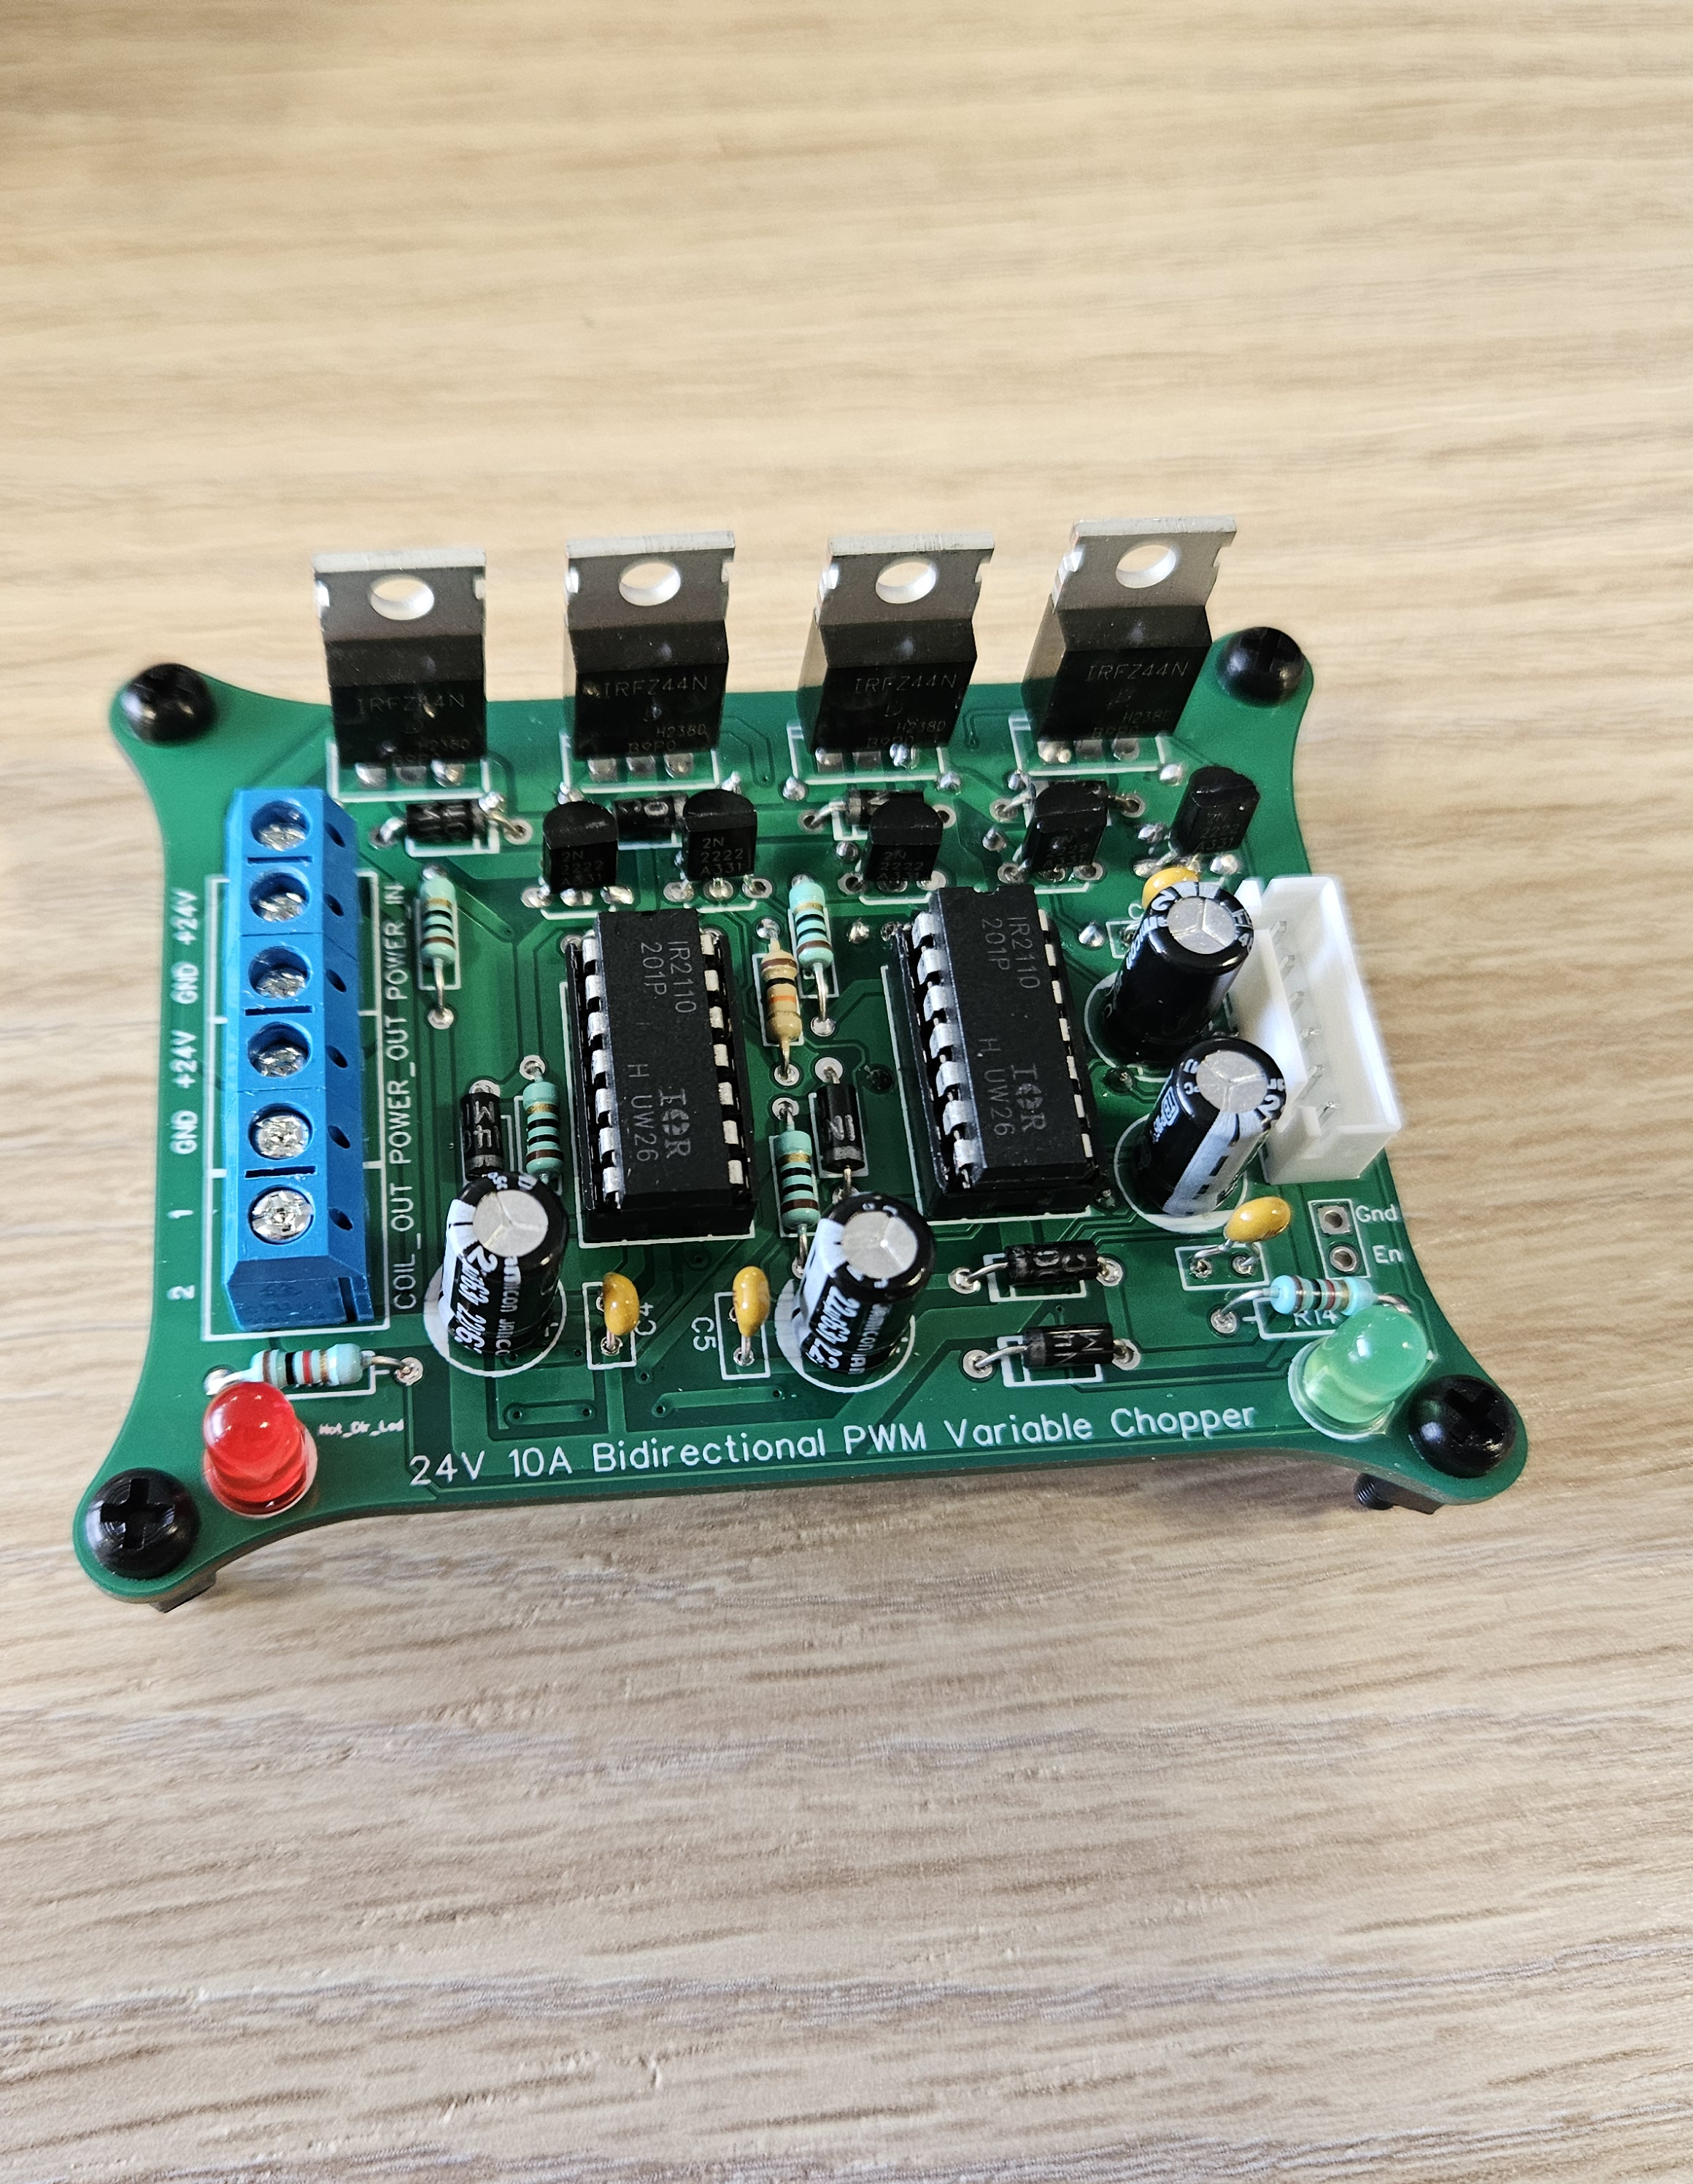
\includegraphics[width=\linewidth]{Images/pcb_reel.jpg}
        \caption{PCB assemblé}
        \label{fig:PCB_3d-2}
    \end{minipage}\hfill
\end{figure}
\section{Électronique de contrôle et liaison avec l'informatique}
    Afin de contrôler les circuits électroniques de puissance, nous avons produit un circuit de contrôle numérique. Nous avons décidé de baser celui-ci autour d'une carte ESP32 car ses caractéristiques correspondait à nos besoins.

    \begin{figure}[H]
    \centering
        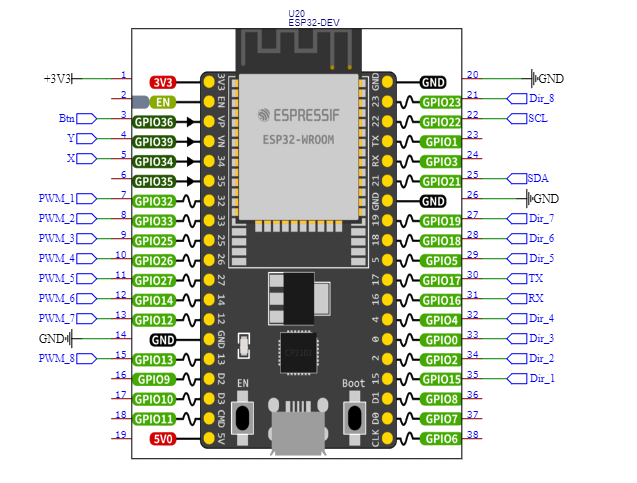
\includegraphics[width = 0.6\textwidth]{Images/ESP32 - pins - clean.png}
        \caption{Disposition des pins de la carte ESP32}
        \label{fig:ESP32 - pins}
    \end{figure}

    \subsection{Communication avec la carte de commande}
        Une connexion UART à 115,200 bauds a été réservée sur la carte de contrôle afin de recevoir des informations sur le mode de contrôle du système (automatique ou manuel) ainsi que sur la puissance à envoyer dans chaque bobine depuis la carte de commande.
        \\\\
        L'information reçue peut avoir 2 formes possibles, soit l'information est simplement un '\verb+0+', dans ce cas, le mode de contrôle est manuel et il n'y a pas d'informations supplémentaires reçues, soit l'information reçue commence par un '1' et ressemble à '\verb+1:DXXX:DXXX:DXXX:DXXX:DXXX:DXXX:DXXX:DXXX+', dans ce cas, le mode de contrôle est automatique et les 'D' et 'XXX' représentent respectivement la direction et la puissance du courant à envoyer dans chaque bobine.

    \subsection{Contrôle numérique de la puissance des bobines}
        Afin de réaliser le contrôle de la puissance du système, nous avons réservé 8 pins PWM ainsi que 8 pins tout-ou-rien en sorties afin de contrôler respectivement le courant électrique ainsi que le sens du courant envoyé dans chaque bobines.
        \\\\
Cependant, il n'est pas envisageable de simplement transmettre les commandes de puissance individuelles à chaque bobine. En effet, si la commande de puissance pour une bobine est considérablement supérieure ou inférieure à la puissance actuellement appliquée à cette bobine, cela entraînerait une variation brutale du courant circulant dans la bobine. Ce changement soudain pourrait provoquer des pics de tension susceptibles de endommager des composants électroniques tels que les transistors MOSFET ou leurs pilotes.
\\\\
Pour cette raison, le programme de contrôle des bobines distingue entre la puissance de commande et la puissance réellement transmise à une bobine. Ainsi, toutes les entrées du programme ne peuvent que modifier la puissance de commande, sans affecter la puissance réelle. La puissance réelle est générée par une fonction qui l'ajuste en fonction de la différence entre la puissance de commande et la puissance réelle. Cette approche permet de modérer la transition de puissance dans les bobines, prévenant ainsi la formation de pics de tension. De plus, il est important de noter que le sens du courant ne peut pas changer de direction tant que la puissance n'est pas nulle.

    \subsection{Pilotage manuel du système}
Afin de déplacer le microrobot, plusieurs méthodes de contrôle ont été envisagées. La première méthode réalisée est le contrôle manuel à l'aide d'un joystick relié à la carte de contrôle via 3 broches d'entrées analogiques : une broche pour le potentiomètre X, une pour le potentiomètre Y et une réservée à l'appui sur le bouton du joystick. 
\\\\
Bien qu'elle ne soit pas nécessaire pour le fonctionnement actuel du projet, la plupart des joysticks proposent une sortie tout-ou-rien pour l'appui du bouton, qui est ici connectée à la carte ESP32 au cas où elle serait utile ultérieurement.
        \\\\
        Pour ce qui est des deux autres entrées analogiques pour les potentiomètre, ces entrées X et Y sont utilisées afin de déterminer la bobine à actionner. Le système est dans ce cas, non pas piloté en choisissant la direction dans laquelle le microrobot doit se déplacer, mais en choisissant la bobine qui doit attirer le microrobot.
        \\\\
        Aussi, puisque la qualité des informations reçues depuis les joysticks analogiques étaient décevante, la solution finalement choisie pour le pilotage manuel du système est maintenant une application Android écrite en Java permettant de contrôler un joystick virtuel, l'information générée est envoyée à la carte de contrôle ESP32 via une connexion Bluetooth, et celle-ci est bien plus précise que le joystick analogique.

        \begin{figure}[H]
    \centering
    \begin{minipage}{0.3\textwidth}
        \centering
        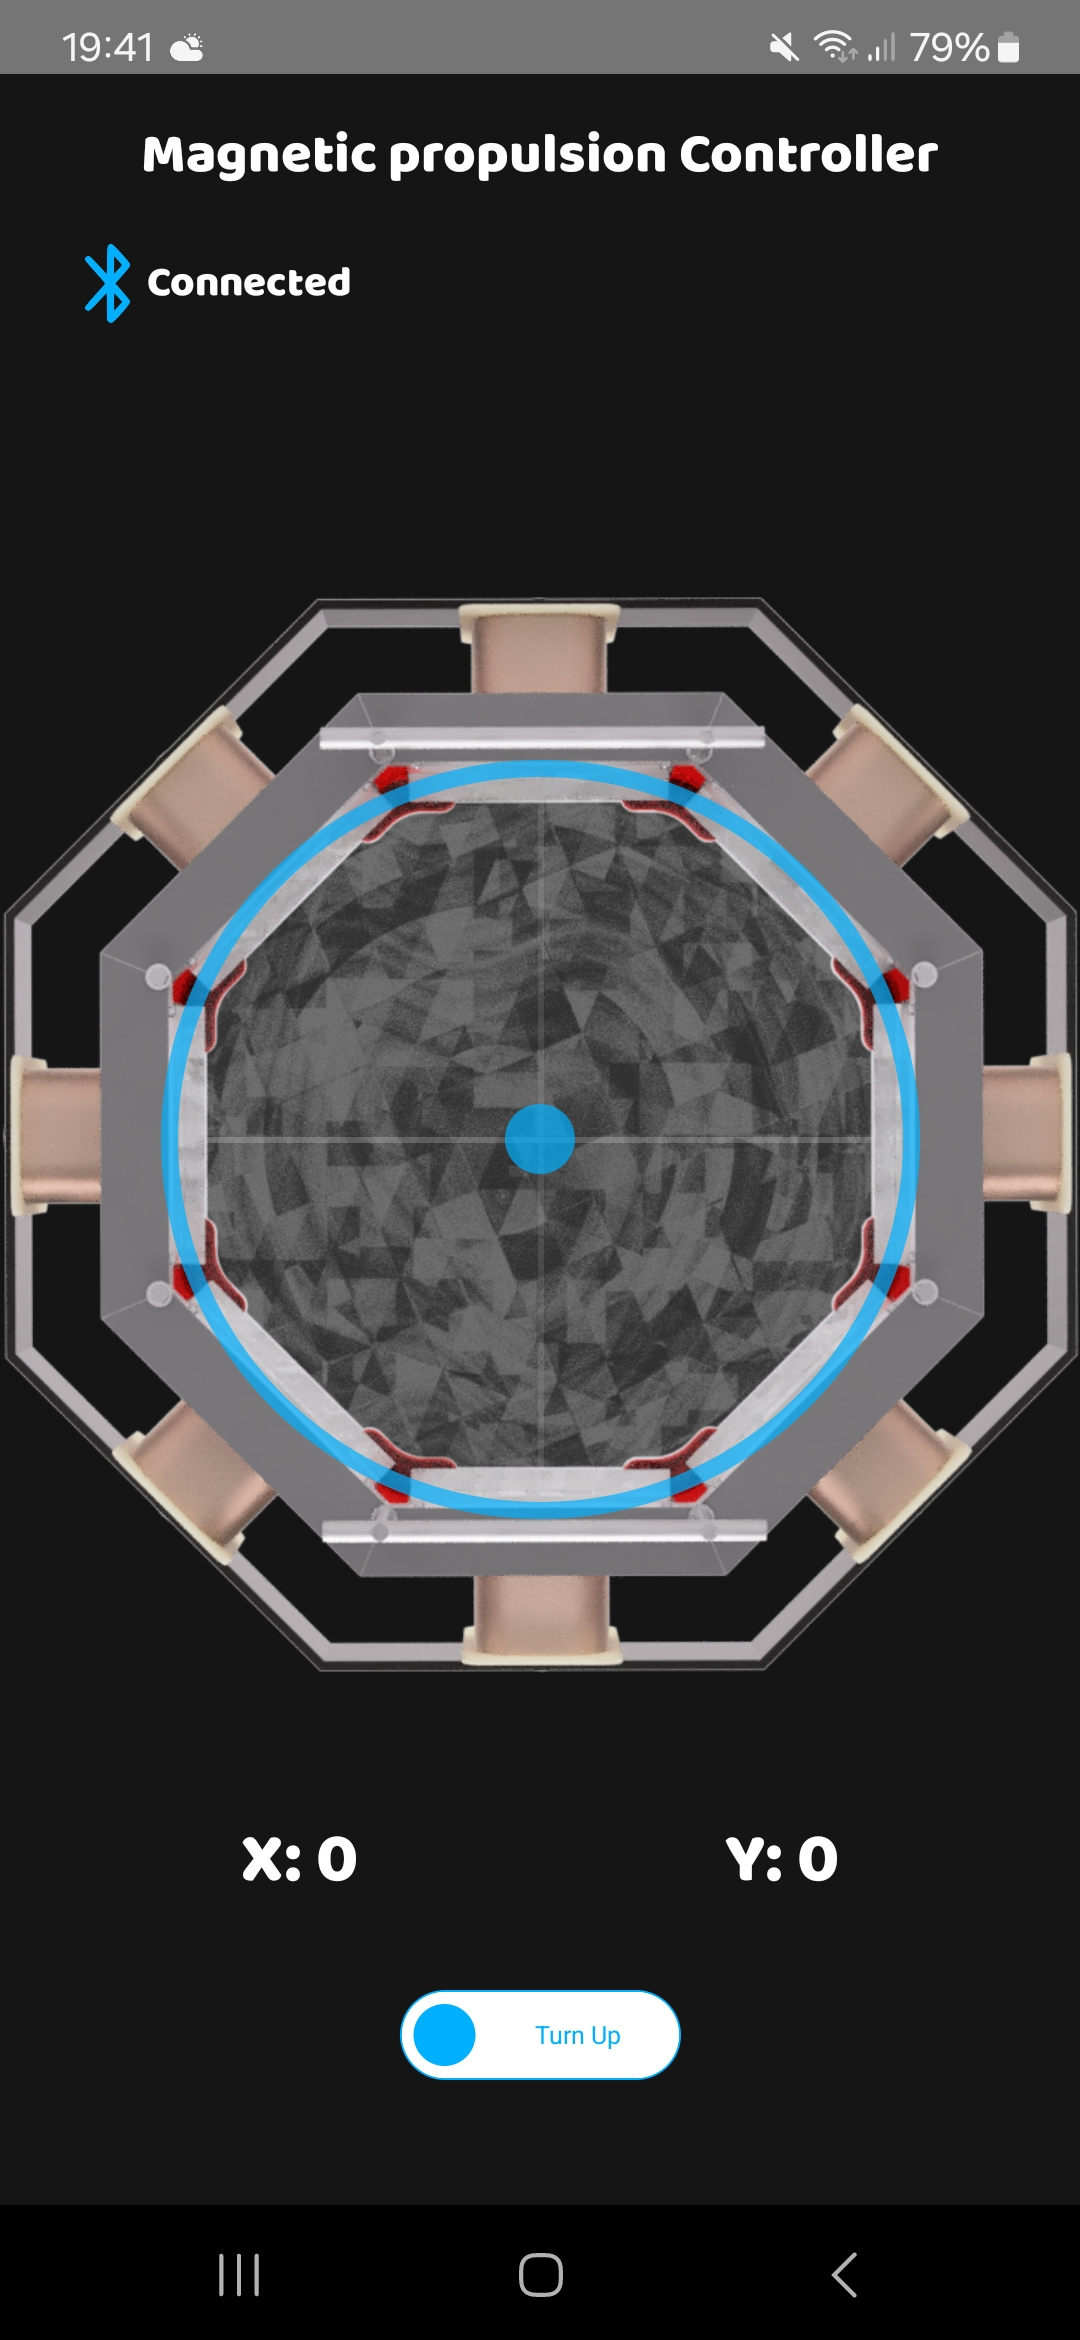
\includegraphics[width=\linewidth]{Images/app1 (3).jpg}

    \end{minipage}\hfill
   \begin{minipage}{0.3\textwidth}
        \centering
        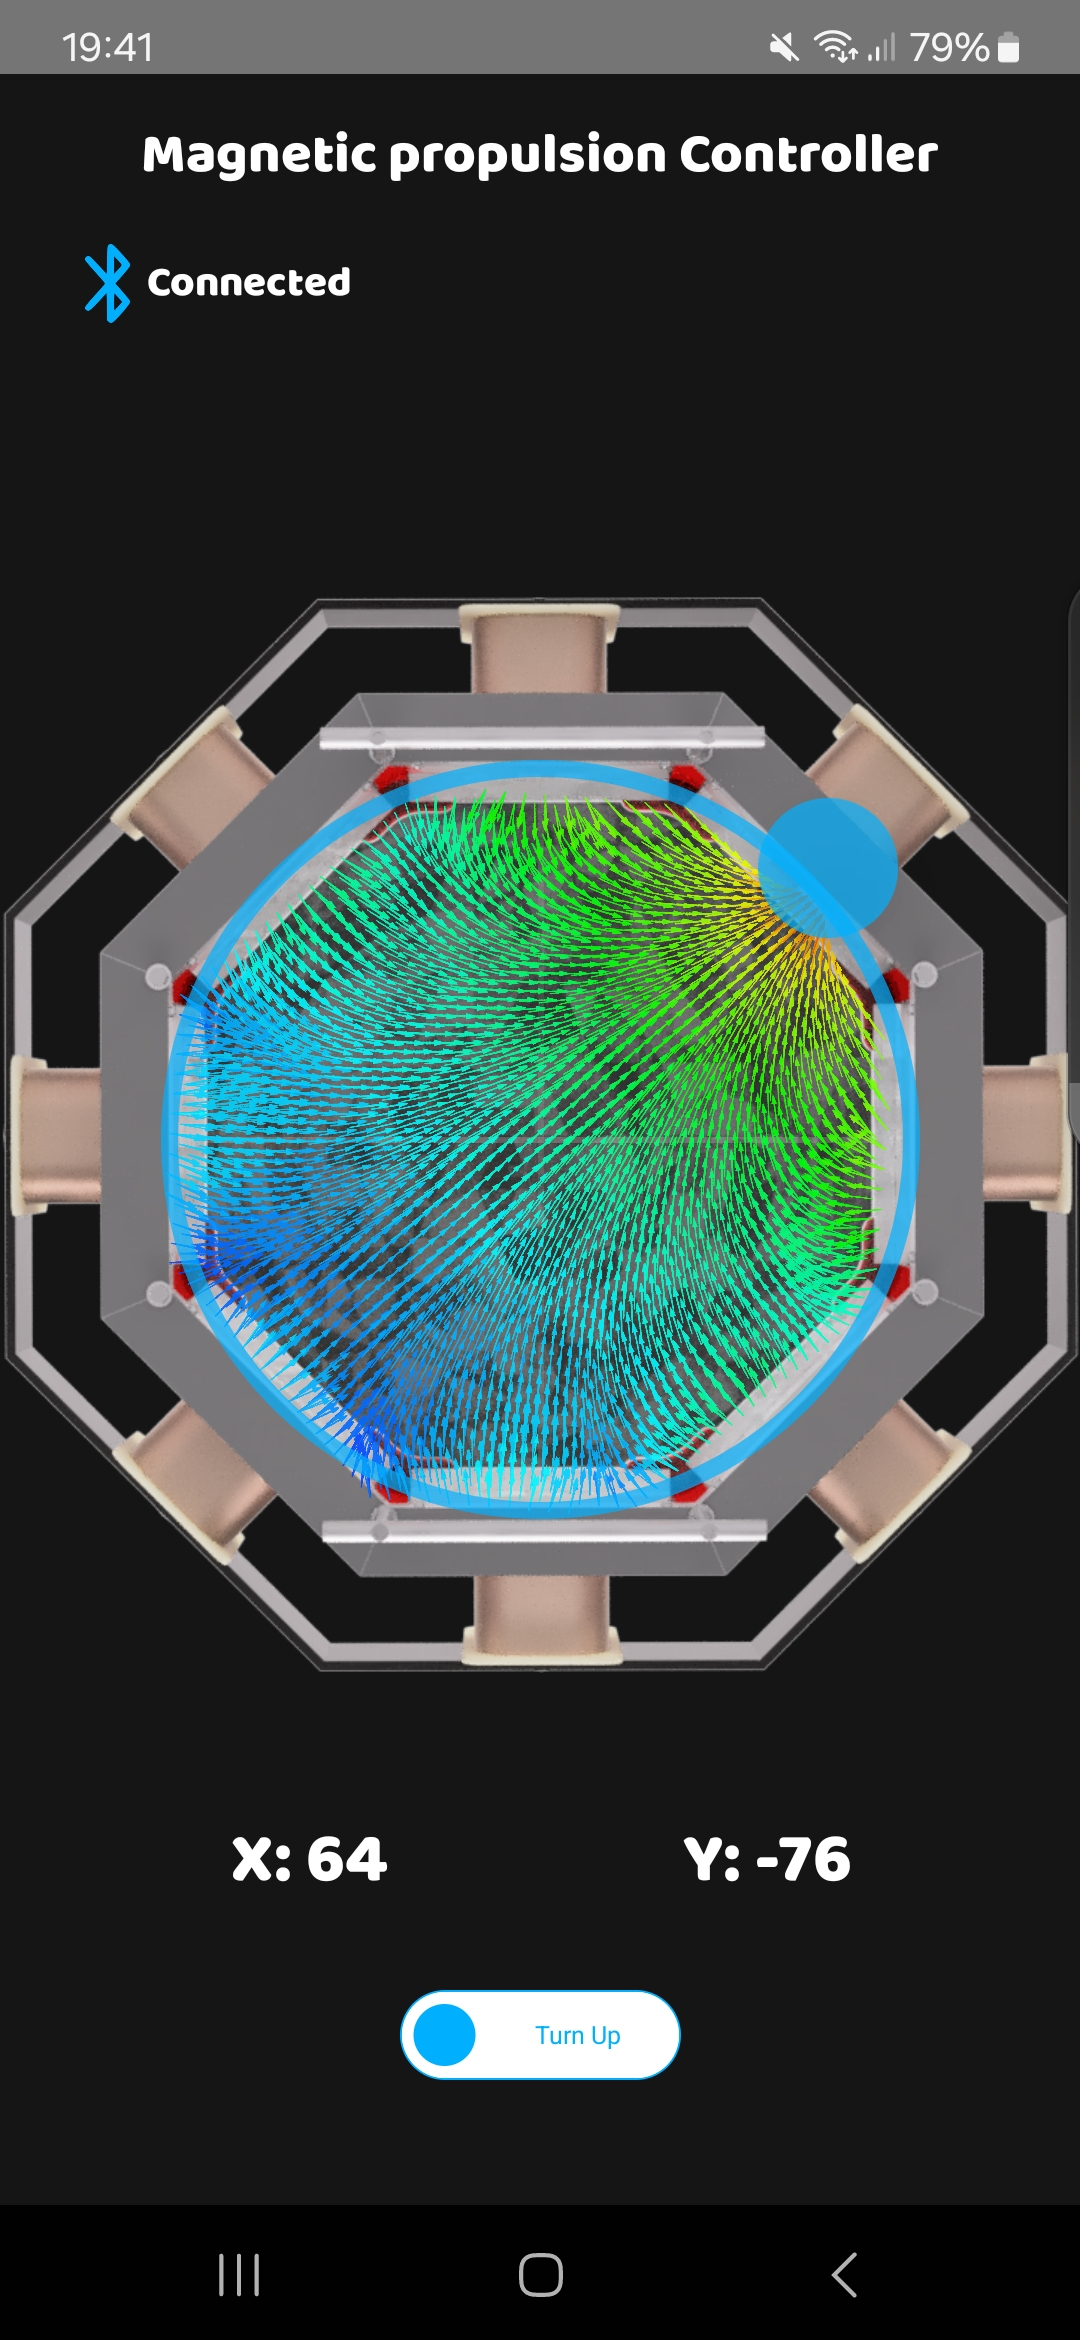
\includegraphics[width=\linewidth]{Images/app1 (1).jpg}

    \end{minipage}\hfill
    \begin{minipage}{0.3\textwidth}
        \centering
        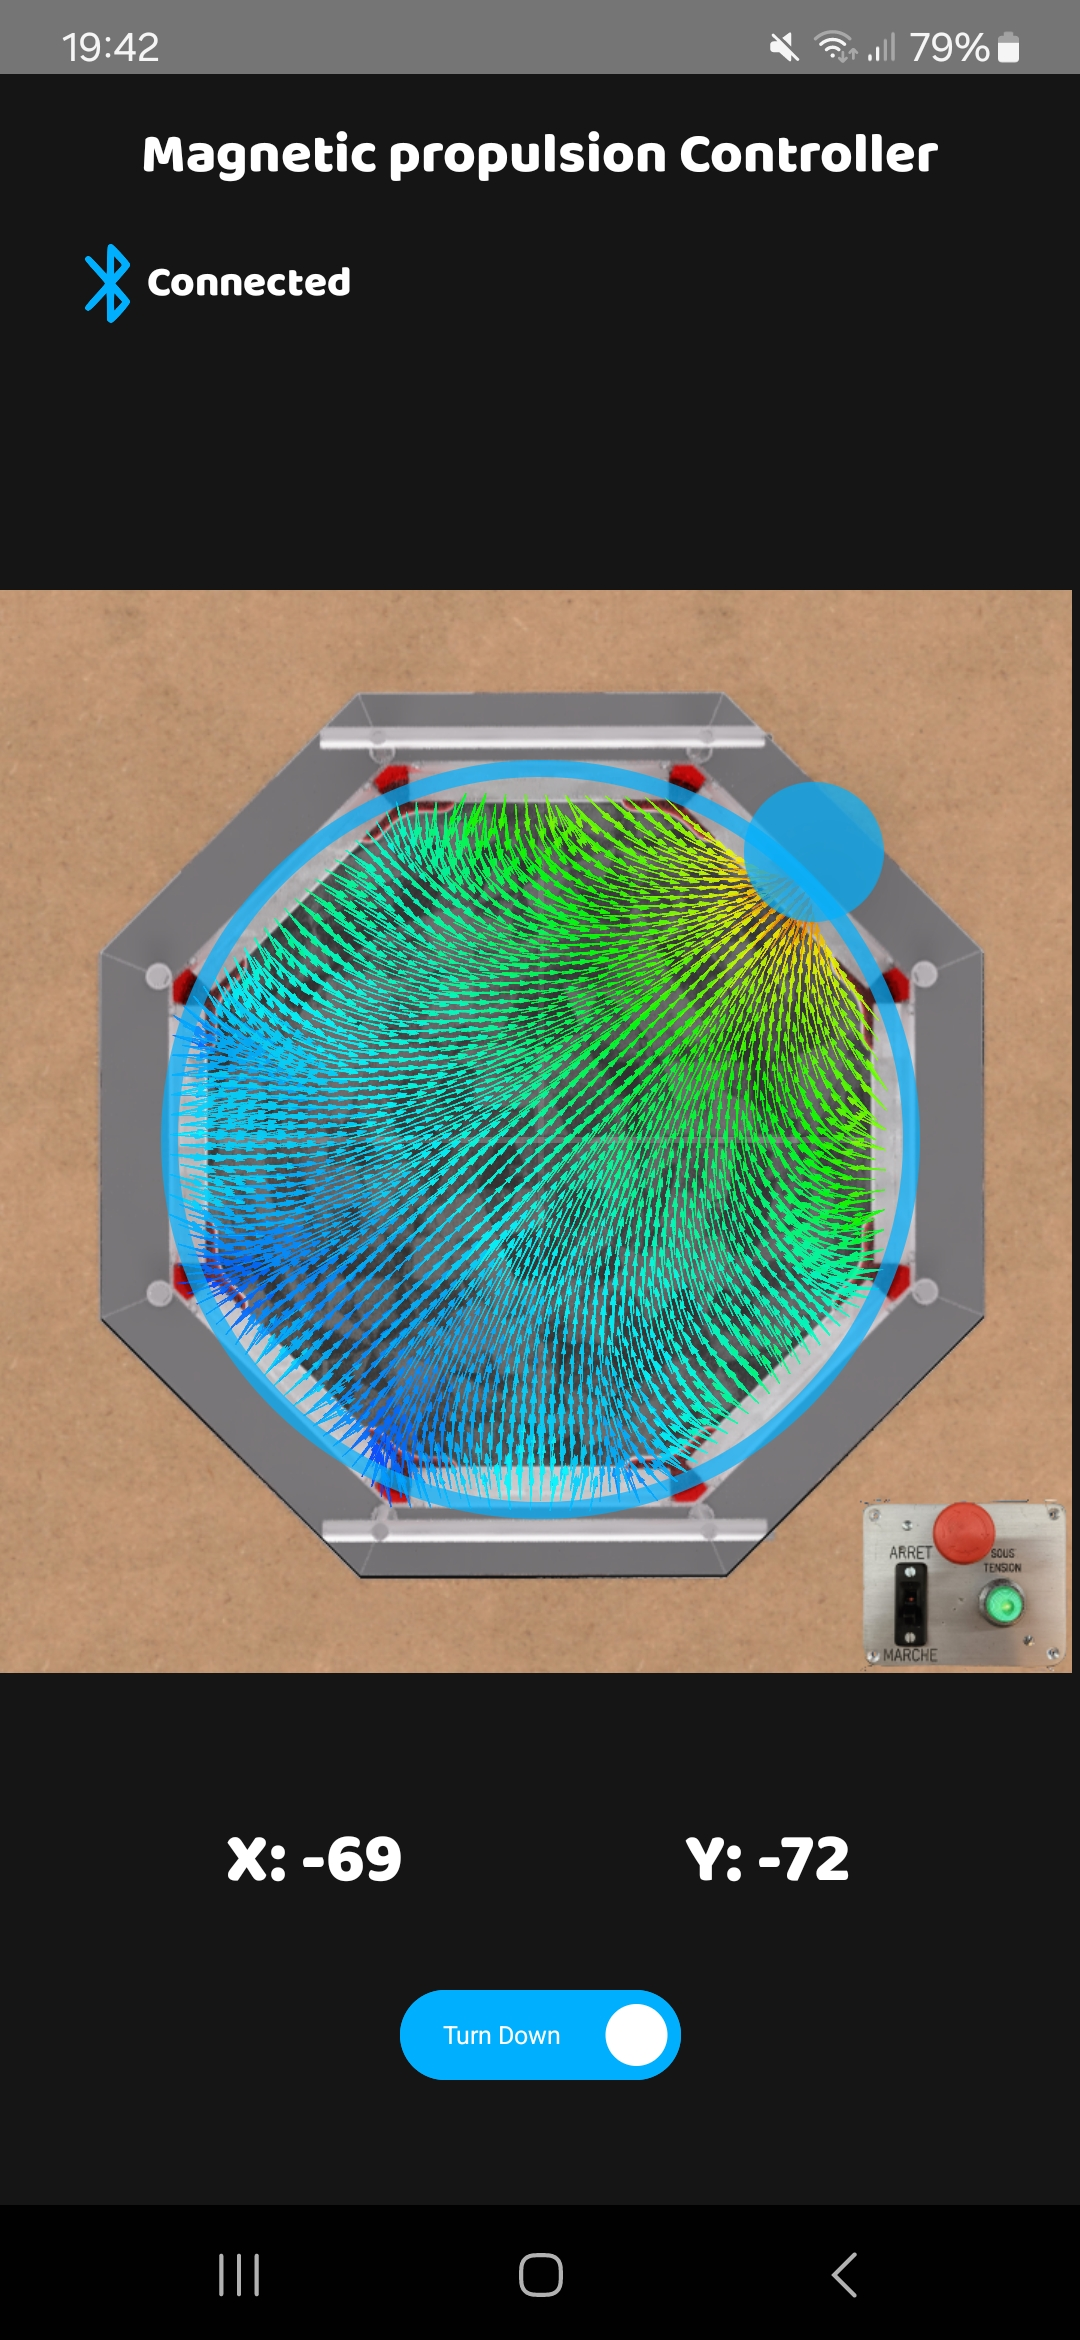
\includegraphics[width=\linewidth]{Images/app1 (2).jpg}

    \end{minipage}\hfill
    \caption{Captures d'écran de l'application}
\end{figure}
        

    \subsection{Pilotage automatique du système}
        La seconde méthode de contrôle mise en œuvre pour déplacer le microdrone est automatique. Les informations sur la puissance à envoyer dans chaque bobine ainsi que la direction du courant à envoyer sont reçues depuis la carte de commande Raspberry Pi.
        \\\\
        Ces puissances reçues sont vérifiées par la carte de contrôle afin que le courant total nécessaire pour alimenter tout le système n'excède pas 40A. Le transformateur utilisé supporte jusqu'à une demande de 50A, néanmoins par sécurité, un fusible supportant jusqu'à 40A a été ajouté en sortie du transformateur.
        \\\\
        Si la somme des courants à envoyer dans chaque bobines est inférieure à 40A, les bobines sont actionnées, dans le cas contraire, elles ne sont pas directement désactivées, car une désactivation brutale pourrait générer un pic de tension, et donc, pourrait endommager le circuit de contrôle.

\section{Système de commande informatique avec reconnaissance de position automatique}
\label{Système de commande informatique}
    Utiliser une caméra reliée à une carte Raspberry Pi est une des solutions les plus simples afin de déterminer la position du microdrone, mais aussi de réaliser le système de guidage automatique du microdrone en calculant la puissance à délivrer dans chaque bobines afin de déplacer le microdrone dans une direction souhaitée.
    \\\\
    Ces informations peuvent ensuite être envoyées à la carte de contrôle de puissance afin d'asservir le système de gestion du courant dans les bobines.

    \subsection{Reconnaissance d'un objet sur une image}
    \label{sec:Reconnaissance d'un objet sur une image}
       Déterminer la position d'un objet sur une image est nécessaire. Pour cela, notre choix s'est porté sur un système de reconnaissance des couleurs en format HSV plutôt qu'à un système de reconnaissance des motifs comme pour les QR codes. Cela s'explique par la nécessité d'économiser de la mémoire, étant donné que les traitements d'images sont lourds en mémoire et qu'une basse résolution a été choisie pour augmenter la vitesse d'exécution de la carte de commande informatique.
\\\\
Aussi, reconnaître les couleurs sur une image au format HSV plutôt qu'au format RGB classique présente un intérêt très important. En effet, le format RGB permet de définir une couleur en fonction du taux de rouge, vert et bleu présents dans celle-ci. Ce format est le plus simple et le plus connu, néanmoins ce n'est pas un format intéressant pour réaliser de la reconnaissance de couleurs.
        \\\\
        En effet, pour reconnaître une couleur nous définissons des limites minimales et maximales autour des valeurs de la couleur qui est recherchée, puis si une couleur est dans cet intervalle, elle est reconnue comme positive à ce test. Par exemple, si nous recherchons du \textcolor{magenta}{magenta} légèrement sombre avec le code RGB suivant : (200, 0, 200), si les limites minimales et maximales de détection sont respectivement (175, 0, 175) ainsi que (225, 0, 225), le système permettra de détecter des teintes de \textcolor{magenta}{magenta} légèrement différentes. Par contre, il détectera aussi des couleurs comme le \textcolor{violet}{violet} et le \textcolor{pink}{rose} dont les codes RGB sont respectivement (175, 0, 225) et (225, 0, 175) comme étant du \textcolor{magenta}{magenta}.
        \\\\
        Ainsi, reconnaître des couleurs au format RGB sur une image signifierait que ce système non seulement ne permettrait pas de reconnaître toutes les teintes de la couleur voulue, mais qu'en plus, il reconnaîtrait des couleurs différentes comme étant celle recherchée.
        \\\\
C'est à ce stade que le format HSV se révèle le plus intéressant. Il définit chaque couleur avec trois valeurs : la teinte, qui représente la position de la couleur sur le cercle chromatique, la saturation, qui détermine l'intensité de la couleur, et la luminosité, qui indique la brillance de la couleur.
        \\\\
       Ce format est préférable car il permet de reconnaître une couleur sur un intervalle de teintes restreint, réduisant ainsi les risques de confondre une autre couleur par erreur. De plus, il permet de reconnaître la couleur désirée dans des plages étendues d'intensité et de luminosité, facilitant ainsi la détection de la couleur souhaitée même dans des conditions variables.
        \\\\
        Une fois que le programme crée un masque de tous les pixels appartenant à l'intervalle de couleurs recherchées, celui-ci définit la position de l'objet détecté comme étant le centre du cercle englobant tous les pixels de ce masque.
    
    \subsection{Reconnaissance de l'environnement de travail}
Avant de déterminer la position du microdrone dans son environnement, il est nécessaire de définir l'environnement dans lequel il évolue. Pour cela, il est plus simple de placer quatre repères sur le plan de travail, marquant ainsi les quatre coins de l'environnement.
\\\\
D'un point de vue technique, lorsque la caméra capture une image, le programme la divise en quatre parties (supérieure gauche, supérieure droite, inférieure gauche et inférieure droite). Ensuite, le programme cherche à reconnaître une balise de couleur facilement identifiable dans chaque partie de l'image. Une fois que ces quatre balises sont reconnues, les quatre coins de l'environnement sont identifiés. L'environnement de travail est donc la surface interne au quadrilatère ainsi formé.
        \\\\
        Une fois l'environnement de travail trouvé, déterminer l'octogone au sein du quel le microdrone pourra se déplacer est assez simple, en effet, les coins de l'octogone sont tous placés à environ 29.29\% et 70.71\% de chaque côtés du quadrilatère représentant l'environnement.

        \begin{figure}[H]
        	\centering
        	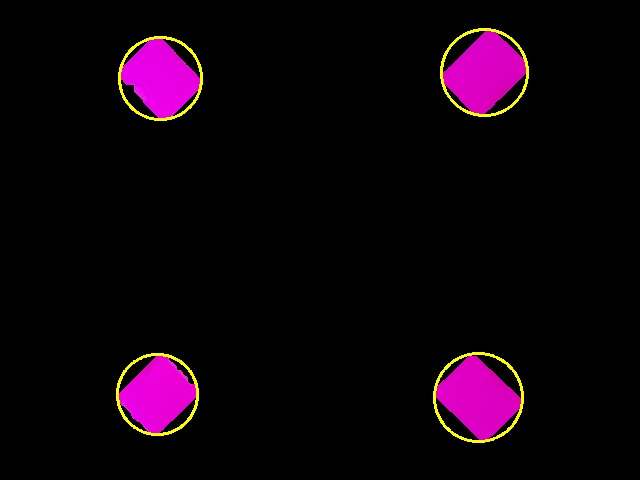
\includegraphics[width = 0.4\textwidth]{Images/view_mask_2}
        	\hspace{1cm}
        	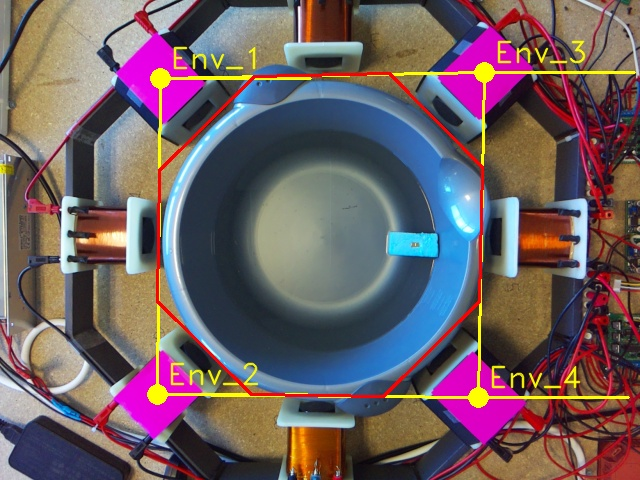
\includegraphics[width = 0.4\textwidth]{Images/view_env}
        	\caption{Détection de l'environnement}
        	\label{ref:Camera environment detection}
        \end{figure}

    \subsection{Calibrage du système de reconnaissance de position}
        Pour calibrer le système de reconnaissance de position, réaliser un système entièrement dynamique capable de déterminer la position d'un point au sein d'un environnement quelque soit la forme de celui-ci aurait été purement ostentatoire, en effet, la caméra sera toujours placée au-dessus de l'environnement de travail, et donc celui-ci apparaîtra toujours carré pour la caméra. Finalement, après plusieurs considérations, il a été déterminé qu'un système de calibrage manuel du système serait à la fois plus simple à concevoir, mais aussi moins gourmand en ressources pour la carte de commande informatique.
        \\\\
        Ce système est assez simple, il s'agit d'aligner les bords de l'environnement de travail avec des droites de calibrage, cela permet de simplifier énormément la reconnaissance de la position du microdrone car celui-ci se déplacera toujours au sein d'un environnement carré.

        \begin{figure}[H]
        	\centering
        	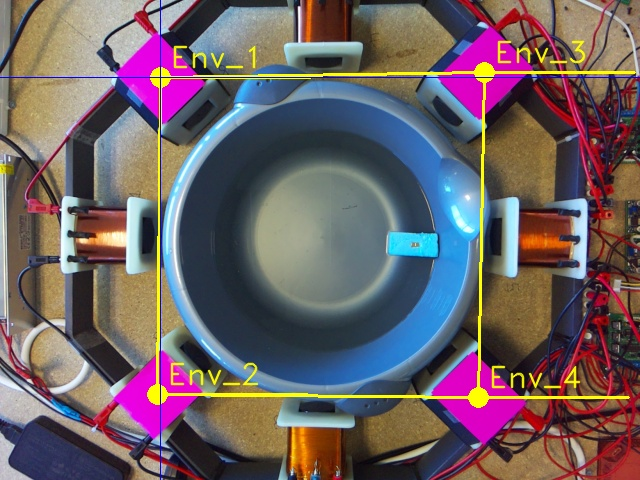
\includegraphics[width = 0.4\textwidth]{Images/view_cal}
        	\caption{Système de calibrage}
        	\label{ref:Camera calibration system}
        \end{figure}

    \subsection{Reconnaissance de position du microdrone}
        Une fois l'environnement de travail reconnu et le calibrage effectué, reconnaître la position du microdrone dans cet environnement devient abordable.
        \\\\
        Premièrement, une couleur est choisie pour que le microdrone se démarque du reste de son environnement, ensuite, la méthode expliquée en \ref{sec:Reconnaissance d'un objet sur une image} est utilisée pour déterminer la position de celui-ci sur l'image capturée par la caméra.
        \\\\
        Pour déterminer la position du microdrone dans l'environnement de travail précédemment déterminé, nous convertissons les coordonnées du microdrone sur l'image en coordonnées au sein de l'environnement de travail (de 0 à 1000 sur les deux axes). Avoir les coordonnées du microdrone au sein de l'environnement de travail comprises entre 0 et 1000 permet de facilement comprendre où le microdrone est situé dans l'environnement.

        \begin{figure}[H]
        	\centering
        	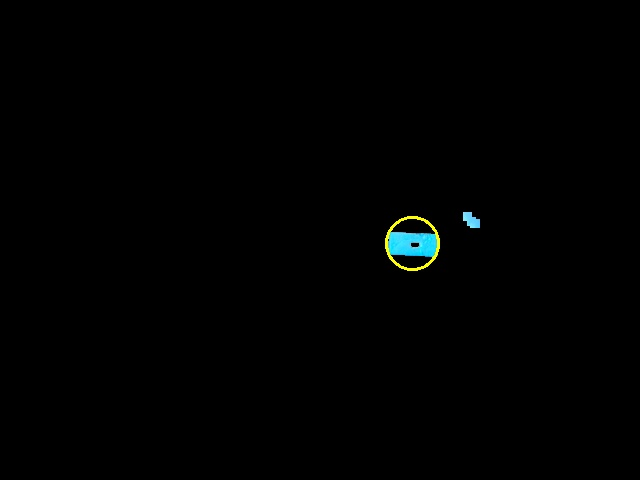
\includegraphics[width = 0.4\textwidth]{Images/view_mask_1}
        	\hspace{1cm}
        	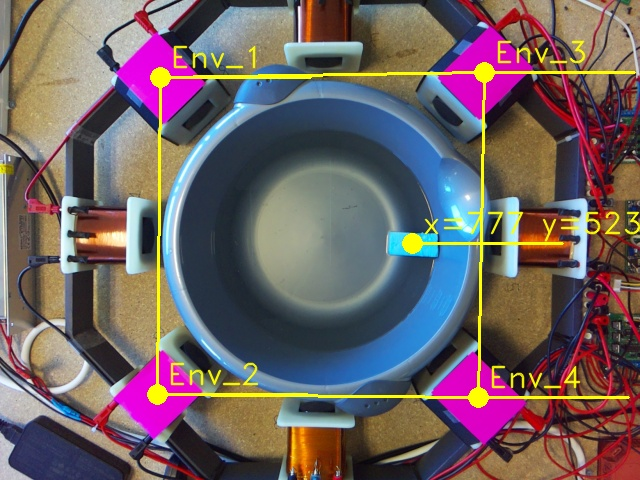
\includegraphics[width = 0.4\textwidth]{Images/view_pos}
        	\caption{Détection de la position du drone}
        	\label{ref:Camera drone position detection}
        \end{figure}

    \subsection{Détermination de la puissance dans chaque bobines}

Une fois toutes les données sur l'environnement et la position du microdrone recueillies, il devient possible de déterminer la puissance nécessaire dans chaque bobine pour déplacer le microdrone dans la direction souhaitée.
        \\\\
        Avec cette direction établie, la bobine à activer pour attirer le microdrone est celle qui se situe le plus dans la direction désirée. Cependant, cette méthode n'est applicable que lorsque le microdrone est éloigné des bords de l'aquarium. En effet, lorsque le microdrone se trouve près des bords de l'aquarium, le contrôle du microdrone est perturbé par des effets de bord qui maintiennent le microdrone collé à la paroi de l'aquarium. Dans cette situation, le contrôle du microdrone est également perturbé par le champ magnétique résiduel dans la structure en acier.
        \\\\
       Pour pallier ces imperfections, il serait envisageable de générer une impulsion de champ magnétique opposé au champ du microdrone. Ainsi, la force magnétique ainsi créée éloignerait le microdrone des bords de l'aquarium ainsi que des bobines les plus proches, sans que le microdrone n'ait le temps de se retourner en raison du moment magnétique.
       
    \subsection{Communication avec la carte de contrôle}
        Quand le mode de contrôle du système ainsi que la puissance et la direction du courant à envoyer dans chaque bobine est déterminée, ces informations sont transmises à la carte de contrôle via une connexion UART à 115,200 bauds.
        \\\\
        Le message prend la forme suivante si le mode de contrôle est manuel:

        \tabto{1cm}\verb+0+
        \\\\
        Le message prend la forme suivante si le mode de contrôle est automatique:
        
        \tabto{1cm}\verb+1:DXXX:DXXX:DXXX:DXXX:DXXX:DXXX:DXXX:DXXX+
        \\
        D : la direction du courant dans chaque bobine
        \\
        XXX : la puissance du courant dans chaque bobine
        \\\\
Il est important de noter qu'il est nécessaire de maintenir la nappe de transfert de données entre la carte de commande et la carte de contrôle, ainsi que la nappe de transfert de données entre la carte de commande et la caméra, à une certaine distance du support en aluminium. Cela permet de limiter au maximum les interactions entre le champ magnétique circulant dans l'espace et les données circulant dans les nappes. Cette problématique a demandé plusieurs heures pour être résolue, notamment lorsque nous avons essayé de comprendre pourquoi des flashs rouges apparaissaient sur le retour vidéo, ce qui avait tendance à faire planter le programme Python. Nous avons finalement compris que cela était dû aux champs magnétiques.


\newpage
\section{Conclusion}
Pour conclure, ce projet se présente comme un démonstrateur dans un environnement simplifié, visant à mettre en avant le potentiel d'utilisation de microdrones avec peu ou pas d'électronique embarquée. Une application envisagée d'un tel système serait dans le domaine médical, permettant d'injecter un microdrone contenant une dose minuscule de médicament directement sur la zone malade grâce à son déplacement à distance. Cependant, une telle application nécessiterait un système beaucoup plus sophistiqué et des ressources de développement incomparables.
\\\\
Malheureusement, tous les objectifs fixés n'ont pas pu être atteints. Les contraintes de délai ont notamment empêché la combinaison du système de reconnaissance de position avec le système de manipulation magnétique. Actuellement, la seule méthode fonctionnelle est de piloter manuellement le microdrone via un téléphone. D'autres complications, telles que les problèmes de rémanence et les effets de bord entre le microdrone et les parois de l'aquarium, n'ont pas eu le temps d'être entièrement résolues. De plus, un point qui nous tenait à cœur était la construction et l'utilisation d'un aquarium sur mesure pour s'intégrer parfaitement au système près des bobines. Bien que les matériaux aient été commandés il y a plusieurs semaines, aucune information n'a été fournie quant à la réalisation de cette commande.
\\\\
Malgré ces défis, le projet a permis de valider l'objectif principal, à savoir la possibilité de déplacer un objet magnétique sans contact mécanique, uniquement à l'aide de champs magnétiques. Des bases structurelles solides ont été posées, qui pourront éventuellement être réutilisées pour se concentrer sur le développement ultérieur d'un contrôle automatisé de précision.
\newpage
\addcontentsline{toc}{section}{Bibliographie}
\bibliographystyle{alpha}
\begin{thebibliography}{30} % Indiquez le nombre maximum de chiffres pour les étiquettes de vos citations

\bibitem{ref1} % Etiquette de la première source
\href{https://theses.hal.science/tel-00952335/document}{Karim Belharet. Navigation prédictive d’un microrobot magnétique : Instrumentation, commande et
validation. Autre. Université d’Orléans, 2013. Français. ffNNT : 2013ORLE2029ff. fftel-00952335f
}\\ % 

\bibitem{ref2} 
\href{https://en.wikipedia.org/wiki/Biot%E2%80%93Savart_law}{Loi de Biot et Savart. (2024 Février 19). Wikipédia}\\ 

\bibitem{ref3} 
\href{https://fr.wikipedia.org/wiki/Bobines_de_Helmholtz}{Bobines de Helmholtz. (2024 mars 18). Wikipédia}\\ 

\bibitem{ref4} 
\href{https://fr.wikipedia.org/wiki/Moment_magn%C3%A9tique}{Moment magnétique. (2023 août 03). Wikipédia}\\ 

\bibitem{ref5} 
\href{https://en.wikipedia.org/wiki/Solenoid}{Solenoid. (2024 février 08). Wikipédia}\\ 

\bibitem{ref6} 
\href{https://fr.wikipedia.org/wiki/Bobines_de_Maxwell}{Bobines de Maxwell. (2023 octobre 29). Wikipédia}\\ 

\bibitem{ref7} 
\href{https://fr.wikipedia.org/wiki/Frottement_fluide}{Frottement fluide. (2024, mars 20). Wikipédia}\\ 

\bibitem{ref8} 
\href{https://repositorio.unicamp.br/acervo/detalhe/911981?guid=1712060927140&returnUrl=\%2fresultado\%2flistar\%3fguid\%3d1712060927140\%26quantidadePaginas\%3d1\%26codigoRegistro\%3d911981\%23911981&i=1}{Henrique Fagundes Gasparoto, Simulação magnetostática 3D por dipolos magnéticos equivalentes. (2013). Universidade Estadual de Campinas. Faculdade de Engenharia Mecânica. Programa de Pós-Graduação em Engenharia Mecânica}\\

\bibitem{ref9} 
\href{https://fr.wikipedia.org/wiki/%C3%89lectroaimant}{Électroaimant. (2024, février 05). Wikipédia}\\ 

\bibitem{ref10} 
\href{https://www.infineon.com/dgdl/Infineon-IRFZ44N-DataSheet-v01_01-EN.pdf?fileId=5546d462533600a40153563b3a9f220d}{DataSheet - IRFZ44N}\\ 

\bibitem{ref11} 
\href{https://docs.rs-online.com/b7d2/A700000006627954.pdf}{DataSheet - TC4427}\\ 

\bibitem{ref12} 
\href{https://docs.rs-online.com/540a/0900766b8006356a.pdf}{DataSheet - IR2110}\\ 

\bibitem{ref13} 
\href{https://www.ti.com/lit/an/slua887a/slua887a.pdf?ts=1712575686076&ref_url=https%253A%252F%252Fwww.google.com%252F}{Bootstrap Circuitry Selection for Half Bridge Configurations. Texas Instruments} \\ 

\bibitem{ref14} 
\href{https://www.digikey.fr/fr/resources/conversion-calculators/conversion-calculator-pcb-trace-width}{Pcb trace width. Digikey}\\ 




\end{thebibliography}

\newpage
\section{Annexes}

\subsection{Schéma des circuits électroniques}
    \begin{figure}[H]
    \centering

    \
        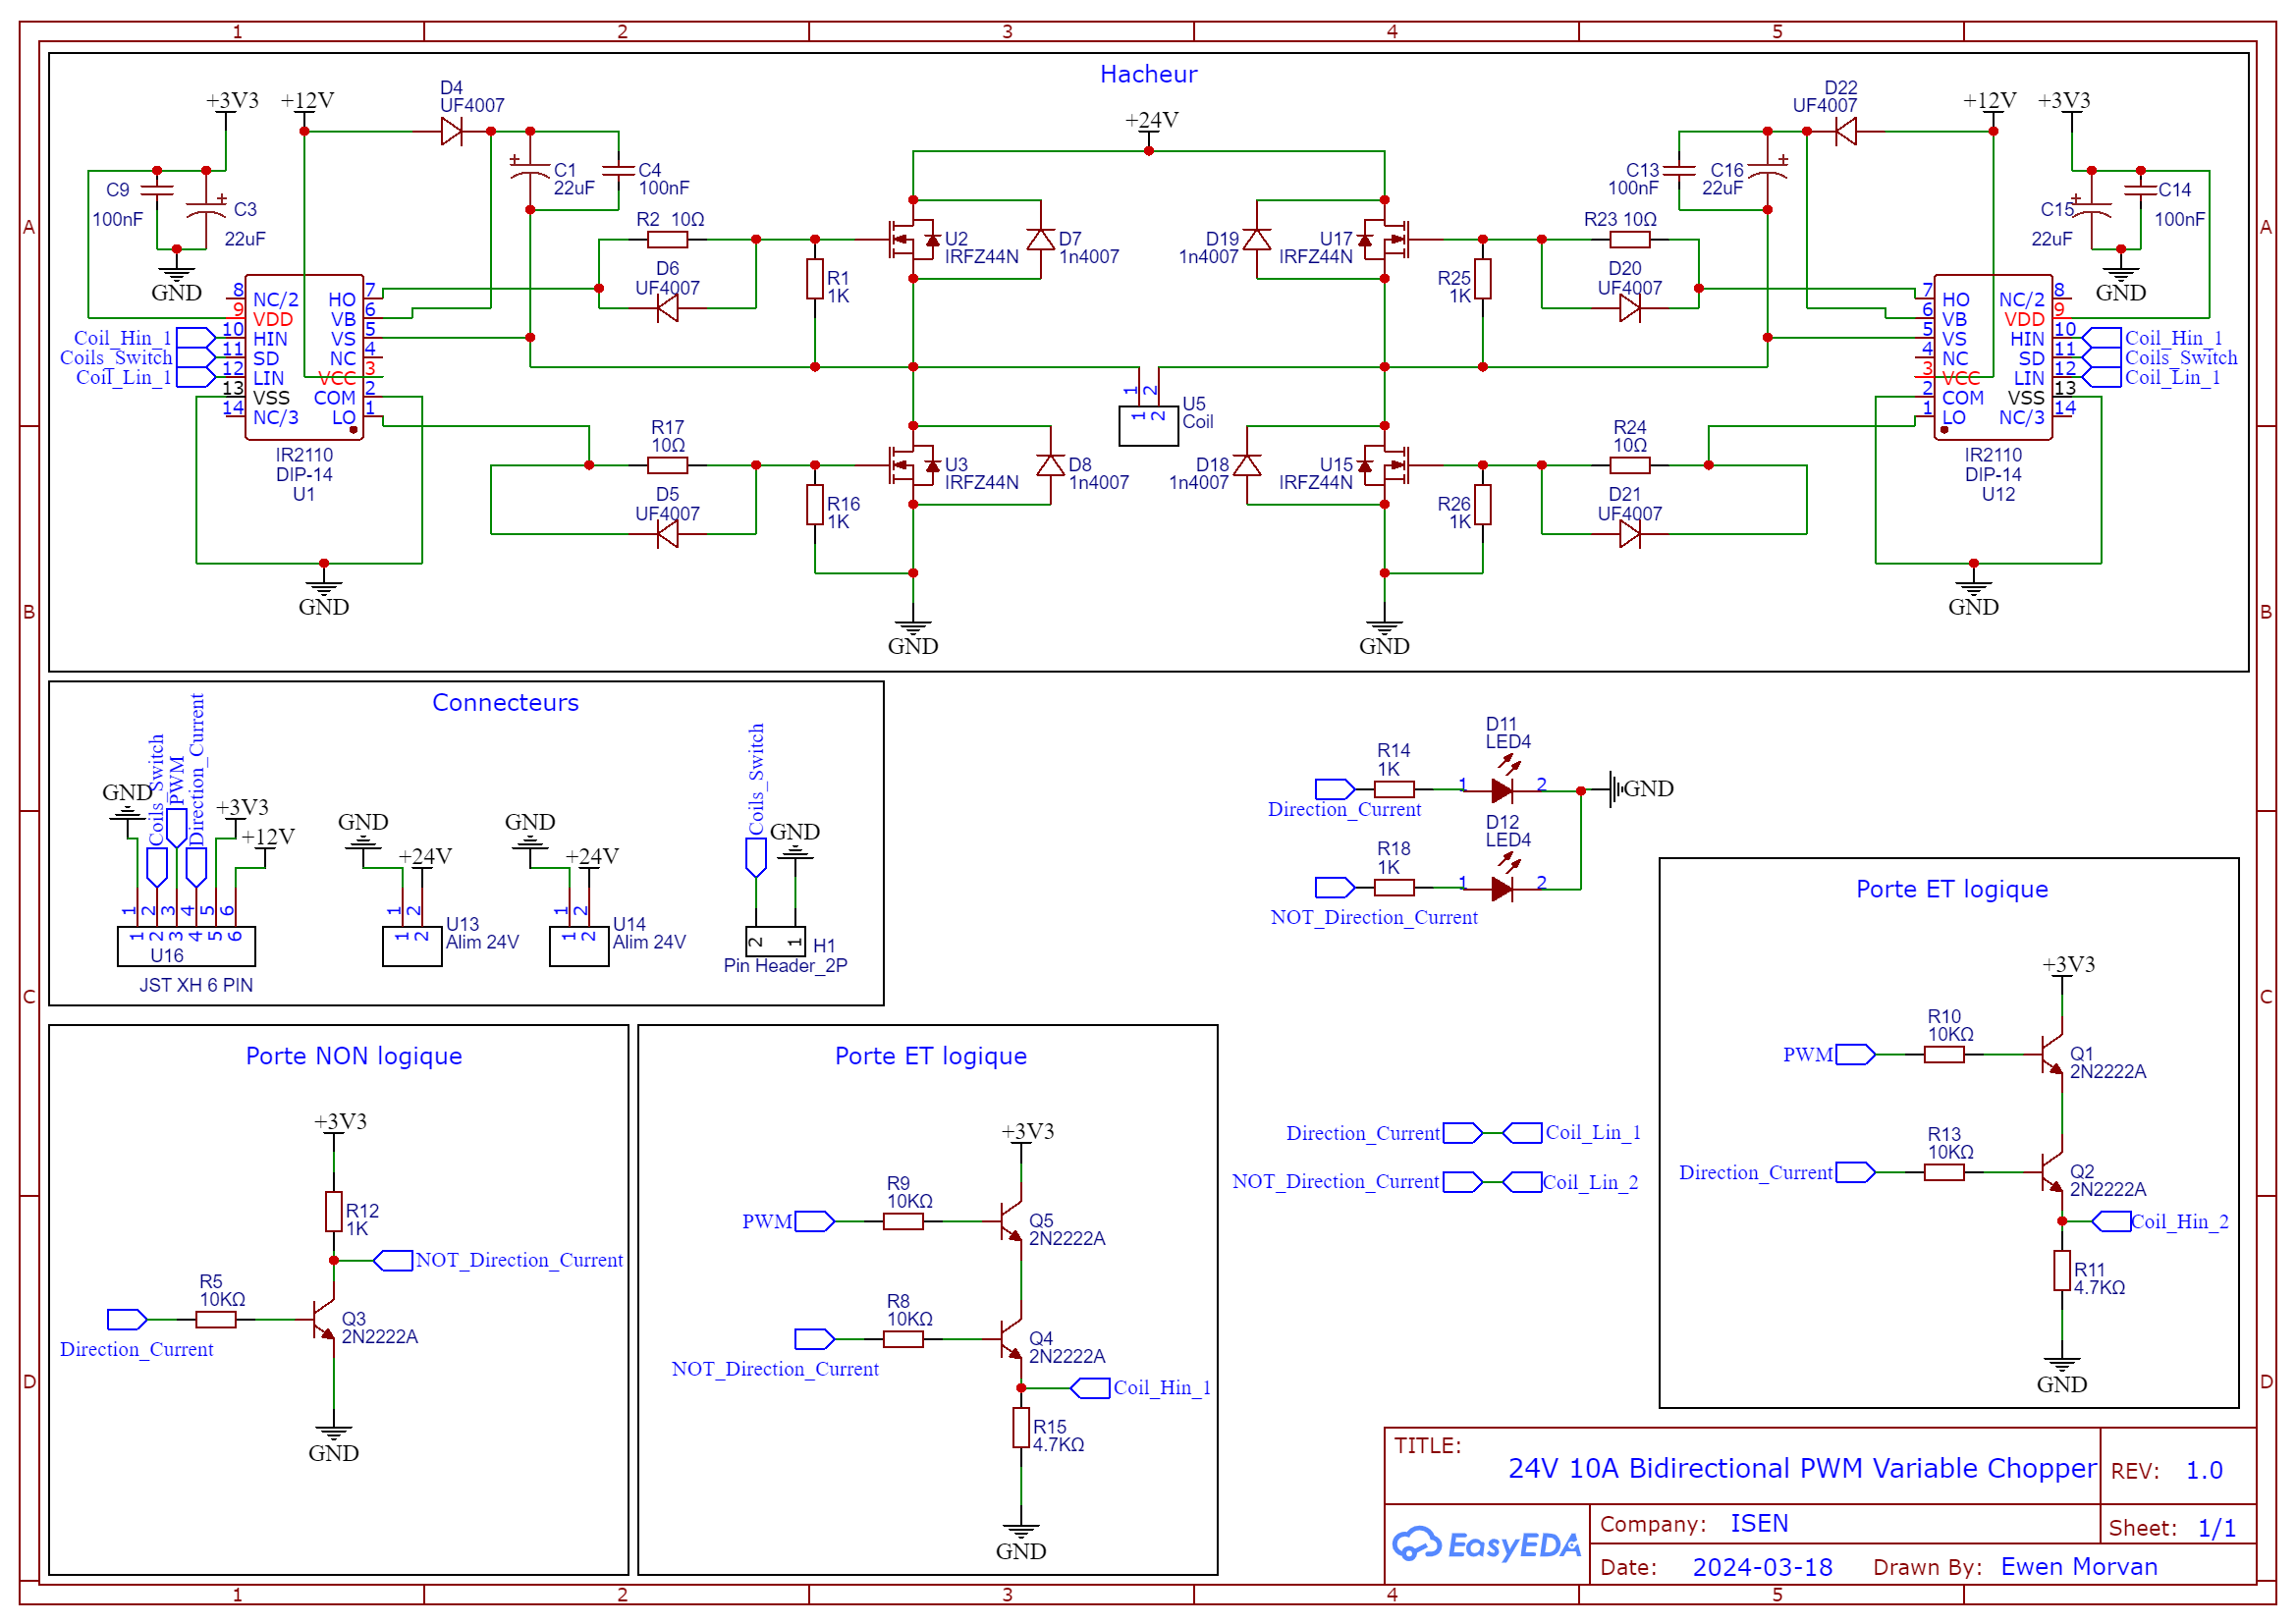
\includegraphics[width = 1.2\textwidth,angle = 90]{Images/Schematic_ProjetM1Isen.png}
        \caption{Schéma d'une carte de puissance}
        \label{fig:schema_carte_puissance}
    \end{figure}
    \newpage
    \begin{figure}[H]
    \centering

        \includegraphics[width = 1.2\textwidth,angle = 90]{Images/Schematic_ProjetM1Isen_controlCard.png}
        \caption{Schéma de la carte de contrôle}
        \label{fig:schema_carte_contrôle}
    \end{figure}





\subsection{Assemblage général du système}

Étant donné que le fournisseur de métal était hors compte et que les limites du budget approchaient, il n'a pas été possible de commander l'acier nécessaire à la conception de la structure. Celui-ci était pourtant indispensable pour la réalisation du projet.
\\L'acier a donc été récupéré gratuitement chez un ferrailleur, qui après quelques négociations, a gentiment offert celui-ci.
\begin{figure}[H]
    \centering
    \begin{minipage}{0.45\textwidth}
    \centering
        \includegraphics[width=\linewidth, angle=270]{Images/photoFabrications/metal_roullier.jpg}
    \end{minipage}\hfill
    \begin{minipage}{0.45\textwidth}
        \centering
        \includegraphics[width=\linewidth, angle=270]{Images/photoFabrications/courses.jpg}
        
    \end{minipage}
    \caption{Acier récupéré gratuitement chez un ferrailleur}
    \label{fig:acier_ferailleur-1}
\end{figure}
\noindent
Il était nécessaire de couper, souder et usiner quelques pièces pour les assembler. À défaut d'avoir les outils à l'ISEN, une demande auprès de M. Mullot a été faite afin d'obtenir l'autorisation de réaliser ce travail dans un atelier en dehors de l'ISEN.
\begin{figure}[H]
    \centering
    \begin{minipage}{0.45\textwidth}
    \centering
        \includegraphics[width=\linewidth, angle=0]{Images/photoFabrications/acier_souder.jpg}
    \end{minipage}\hfill
    \begin{minipage}{0.45\textwidth}
        \centering
        \includegraphics[width=\linewidth, angle=0]{Images/photoFabrications/tour.jpg}
        
    \end{minipage}
    \caption{Fabrication des différentes pièces}
    \label{fig:acier_ferailleur-2}
\end{figure}
\begin{figure}[H]
    \centering
    \begin{minipage}{0.3\textwidth}
    \centering
        \includegraphics[width=\linewidth, angle=0]{Images/photoFabrications/octogone1.jpg}
    \end{minipage}\hfill
    \begin{minipage}{0.3\textwidth}
     
        \includegraphics[width=\linewidth, angle=270]{Images/photoFabrications/support_bobine.jpg}
        
    \end{minipage}
    \begin{minipage}{0.3\textwidth}
        \centering
        \includegraphics[width=\linewidth, angle=0]{Images/photoFabrications/octogone2.jpg}
        
    \end{minipage}
    \caption{Assemblage des différentes pièces}
    \label{fig:acier_ferailleur-3}
\end{figure}
\noindent
Une fois la structure octogonale métallique réalisée, elle a été ramenée à l'ISEN afin d'y intégrer les bobines et effectuer quelques tests.
    \begin{figure}[H]
    \centering
        \includegraphics[width = 0.45\textwidth]{Images/photoFabrications/test1.jpg}
        \caption{Premiers tests avec les bobines et une alimentation de laboratoire}
        \label{fig:test1}
    \end{figure}
\noindent
Pour permettre le positionnement de la caméra au-dessus de la structure, un simple pied a été fabriqué avec des profilés aluminium disponibles dans la salle de robotique. Et pour que la caméra puisse reconnaître l'environnement de travail, des papiers de couleur ont été collés sur 4 des bobines.
\begin{figure}[H]
    \centering
    \begin{minipage}{0.45\textwidth}
    \centering
        \includegraphics[width=\linewidth, angle=0]{Images/photoFabrications/octogone3.jpg}
    \end{minipage}\hfill
    \begin{minipage}{0.45\textwidth}
        \centering
        \includegraphics[width=\linewidth, angle=0]{Images/photoFabrications/test2.jpg}
        
    \end{minipage}
    \caption{Test de la reconnaissance automatique par caméra}
    \label{fig:test2}
\end{figure}
\noindent
Afin de présenter le projet sous sa forme finale (une table avec uniquement un bassin et le microdrone évoluant comme par magie), une planche percée d'un trou central pour l'aquarium a été ajoutée. L'objectif étant d'installer l'ensemble du système et de l'électronique en dessous, de sorte qu'une fois retournée, tout soit dissimulé.
\begin{figure}[H]
    \centering
    \begin{minipage}{0.45\textwidth}
    \centering
        \includegraphics[width=\linewidth, angle=0]{Images/photoFabrications/assemblage1.jpg}
    \end{minipage}\hfill
    \begin{minipage}{0.45\textwidth}
        \centering
        \includegraphics[width=\linewidth, angle=0]{Images/photoFabrications/assemblage2.jpg}
        
    \end{minipage}
    \caption{Assemblage et fixation du projet sur une planche}
    \label{fig:assemblage1}
\end{figure}
\begin{figure}[H]
    \centering
    \begin{minipage}{0.45\textwidth}
    \centering
        \includegraphics[width=\linewidth, angle=0]{Images/photoFabrications/final (2).jpg}
    \end{minipage}\hfill
    \begin{minipage}{0.45\textwidth}
        \centering
        \includegraphics[width=\linewidth, angle=0]{Images/photoFabrications/final.jpg}
        
    \end{minipage}
    \caption{Assemblage de l'électronique}
    \label{fig:assemblage2}
\end{figure}

\begin{figure}[H]
    \centering
    \begin{minipage}{0.32\textwidth}
    \centering
        \includegraphics[width=\linewidth, angle=0]{Images/photoFabrications/final (1).jpg}
    \end{minipage}\hfill
    \begin{minipage}{0.32\textwidth}
    \centering
        \includegraphics[width=\linewidth, angle=0]{Images/photoFabrications/final (4).jpg}
    \end{minipage}\hfill
    \begin{minipage}{0.32\textwidth}
        \centering
        \includegraphics[width=\linewidth, angle=0]{Images/photoFabrications/final (3).jpg}
        
    \end{minipage}
    \caption{Projet final}
    \label{fig:assemblage3}
\end{figure}
\noindent
Voici le projet dans sa version terminée, réalisée dans le temps imparti. L'aquarium prévu, tel qu'illustré sur les plans 3D, n'a malheureusement pas pu être concrétisé. À sa place, la bassine initialement destinée à des tests temporaires est restée en place.

\subsection{Ressources numériques}
Tous les codes sources peuvent être retrouvés sur github \href{https://github.com/JeanLeBris/Drone_Magnetic_Telepropulsion}{ici}.
\\\\
Les modèles 3D SolidWorks réalisés pour ce projet sont disponibles \href{https://grabcad.com/library/tele-propulsion-et-telecommande-magnetique-de-drones-de-surface-1}{ici}.

%\addtocontents{toc}{\protect\setcounter{tocdepth}{0}}
\subsection*{Message à toute personne souhaitant réutiliser ou améliorer ce projet}
Pour préserver l'intégrité des cartes de puissance, veuillez faire preuve d'une grande délicatesse lors de leur programmation. Un changement brusque de puissance ou un revirement de direction du courant alors que l'intensité circulant dans les bobines est supérieure à zéro pourrait être destructeur. Il est recommandé d'utiliser une alimentation de laboratoire avec limitation de courant pour tous les tests. Utilisez l'alimentation de 50A uniquement lorsque vous êtes entièrement sûr et certain que tout fonctionne correctement. Cette alimentation ne pardonne pas les erreurs concernant les cartes de puissance.

Si vous souhaitez réutiliser l'application de contrôle, le code source JAVA est disponible sur le github mentionné précédemment. L'objectif du projet n'était absolument pas de développer une belle application de contrôle bien structurée. Elle a simplement été réalisée en urgence un soir, car la précision des joysticks Arduino bon marché était catastrophique et il n'était plus envisageable d'en acheter un meilleur dans le délai imparti. Le code Java est donc fourni tel quel, sans documentation ni bonne structure. Il suffit de l'importer dans Android Studio pour le compiler et l'installer sur votre téléphone. Si vous possédez un iPhone, malheureusement, il faudra tout recommencer en Swift.

\end{document}